\documentclass[a4paper,11pt]{book}
\title{Applications of boundary tracing in thermal radiation and capillarity}
\author{Conway}

%%%%%%%%%%%%%%%%%%%%%%%%%%%%%%%%%%%%%%%%%%%%%%%%%%%%%%%%%%%%%%%%
% Customisation
%%%%%%%%%%%%%%%%%%%%%%%%%%%%%%%%%%%%%%%%%%%%%%%%%%%%%%%%%%%%%%%%

% Margins
%   NOTE: a 4cm inner margin is required for binding
\usepackage[
  bindingoffset=2cm,
  inner=2cm,
  outer=2.5cm,
  top=3cm,
  bottom=2.7cm,
]{geometry}

% Slightly-more-than-one spacing
% --------
% NOTE: for 11pt font, \onehalfspacing is defined as \setstretch{1.213}.
% See <https://github.com/rf-latex/setspace/blob/02cf9e0/setspace.sty#L350>.
% The general consensus is that
% (1) nobody knows what one-and-a-half and double spacing mean, and
% (2) large line spacing is ugly.
% See <https://tex.stackexchange.com/a/13803>.
\usepackage{setspace}
\setstretch{1.13}

% Heading styles
% --------
% Larger part headings label
% Smaller chapter headings
\usepackage{titlesec}
\titleformat{\part}[display]%
  {\setstretch{1.5}\normalfont\Huge\bfseries\filcenter}%
  {\partname~\thepart}%
  {0em}%
  {}
\titleformat{\chapter}[display]%
  {\setstretch{1}\normalfont\huge\bfseries\filright}%
  {\chaptertitlename~\thechapter}%
  {0em}%
  {}
\titlespacing*{\chapter}{0em}{0em}{3.3em}

% Number subsubsections
\setcounter{secnumdepth}{3}

% Table of contents
% --------
% Include Bibliography etc. but exclude Table of contents
% Include subsubsections
\usepackage[nottoc]{tocbibind}
\setcounter{tocdepth}{3}

% Citations ordered by number with whitespace stripped for keys
\usepackage{cite}

% Symbols for footnotes
\renewcommand*{\thefootnote}{\fnsymbol{footnote}}

%%%%%%%%%%%%%%%%%%%%%%%%%%%%%%%%%%%%%%%%%%%%%%%%%%%%%%%%%%%%%%%%
% Mathematical notation
%%%%%%%%%%%%%%%%%%%%%%%%%%%%%%%%%%%%%%%%%%%%%%%%%%%%%%%%%%%%%%%%

% General symbols ("\;" etc.)
\usepackage{amsmath}

% Paired delimiters ("\abs" etc.)
\usepackage{mathtools}

% Boxed equation emphasis
\usepackage{empheq}

% Physical units
\usepackage{siunitx}

%%%%%%%%%%%%%%%%%%%%%%%%%%%%%%%%%%%%%%%%%%%%%%%%%%%%%%%%%%%%%%%%
% Figures
%%%%%%%%%%%%%%%%%%%%%%%%%%%%%%%%%%%%%%%%%%%%%%%%%%%%%%%%%%%%%%%%

% External graphics
\usepackage{graphicx}

% Figures directory
\graphicspath{{figures/}}

% Subfigures with captions
\usepackage{subcaption}

% Centred figure content (with same label as file name)
%   #1  [\includegraphics options] default "width=\textwidth"
%   #2  {\includegraphics file name}
%   #3  {caption}
\newcommand{\centredfigurecontent}[3][width=\textwidth]{%
  \centering
  \includegraphics[#1]{#2}
  \caption{#3}
  \label{fig:#2}
}

%%%%%%%%%%%%%%%%%%%%%%%%%%%%%%%%%%%%%%%%%%%%%%%%%%%%%%%%%%%%%%%%
% Referencing
%%%%%%%%%%%%%%%%%%%%%%%%%%%%%%%%%%%%%%%%%%%%%%%%%%%%%%%%%%%%%%%%

% Hyperlinks
\usepackage[
  hidelinks,
  bookmarksopen=true,
  bookmarksopenlevel=0,
]{hyperref}

% Top-level backmatter bookmarks
\usepackage{bookmark}

% URLs
\let\bareurl\url
\newcommand*{\urlopen}{\nolinkurl{<}}
\newcommand*{\urlclose}{\nolinkurl{>}}
\renewcommand*{\url}[1]{\urlopen\bareurl{#1}\urlclose}

% DOIs
\newcommand*{\doidomain}{https://doi.org/}
\newcommand*{\doi}[1]{\url{\doidomain #1}}

%%%%%%%%%%%%%%%%%%%%%%%%%%%%%%%%%%%%%%%%%%%%%%%%%%%%%%%%%%%%%%%%
% Math macros
%%%%%%%%%%%%%%%%%%%%%%%%%%%%%%%%%%%%%%%%%%%%%%%%%%%%%%%%%%%%%%%%

% Optional superscript
\newcommand*{\optionalsup}[1]{%
  \ifx \relax #1\relax
  \else
    ^{#1}%
  \fi
}

% Optional subscript
\newcommand*{\optionalsub}[1]{%
  \ifx \relax #1\relax
  \else
    _{#1}%
  \fi
}

% Opposite of \nonumber
\newcommand*{\yesnumber}{\addtocounter{equation}{1}\tag{\theequation}}

% Mathop spacing
\newcommand*{\mathopspace}{\mathop{}\!}

% Horizontal space between math and text in a display equation
\newcommand*{\eqnspace}{\qquad}

% More vertical space for lines containing fractions etc.
\newcommand*{\tallspace}{0.3em}

% Asymptotically
\newcommand*{\asy}{\sim}

% Identically equal to
\newcommand*{\ideq}{\equiv}

% Approximately equal to
\renewcommand*{\approx}{\simeq}

% Bold vectors
\renewcommand*{\vec}[1]{\boldsymbol{\mathbf{#1}}}

% Bracketing
% --------
% Style guide for optional sizing argument:
%   NOTHING       for text-height content (or just use ordinary brackets)
%   [\bulkysize]  for text-height content which is bulky or long
%   [\dersize]    for text-height content which a fraction-height derivative
%                     (\tder, \pder, etc.) is acting upon
%   *             for everything else (including superscript-height content)
% See <https://tex.stackexchange.com/a/565199>.
\DeclarePairedDelimiter{\curlybr}{\{}{\}}
\DeclarePairedDelimiter{\roundbr}{(}{)}
\DeclarePairedDelimiter{\squarebr}{[}{]}
\newcommand{\bulkysizel}{\bigl}
\newcommand{\bulkysizer}{\bigr}
\newcommand{\dersizel}{\Bigl}
\newcommand{\dersizer}{\Bigr}

% Evaluation
% --------
% Style guide for sizing argument (do not omit since left delimiter is "."):
%   [\textsize]   for text-height or superscript-height content
%   *             for everything else
\DeclarePairedDelimiter{\eval}{.}{\rvert}
\newcommand{\textsizel}{\bigl}
\newcommand{\textsizer}{\bigr}

% Del operator
\newcommand*{\del}{\mathopspace\vec{\nabla}}

% Partial differential
\newcommand*{\pd}{\mathopspace\partial}

% Partial derivative
% --------
%   #1  [order] default ""
%   #2  {dependent variable}
%   #3  {independent variable}
\newcommand*{\pder}[3][]{
  \frac{\pd\optionalsup{#1}#2}{{\pd #3}\optionalsup{#1}}
}

% Total differential
% --------
% Style guide:
%   {\td x}   for the denominator of a derivative after "/"
%             (see <https://tex.stackexchange.com/a/68303>)
%   {\td s}^2 for the square of a differential
%             with thin space "\," before or after as necessary
\newcommand*{\td}{\mathopspace\mathrm{d}}

% Total derivative
% --------
%   #1  [order] default ""
%   #2  {dependent variable}
%   #3  {independent variable}
\newcommand*{\tder}[3][]{
  \frac{\td\optionalsup{#1}#2}{{\td #3}\optionalsup{#1}}
}

% Component of a vector
\newcommand*{\comp}[2]{#1_{#2}}

% Cross product
\newcommand*{\crossp}{\boldsymbol{\times}}

% Dot product
\newcommand*{\dotp}{\boldsymbol{\cdot}}

% Absolute value
\DeclarePairedDelimiter{\abs}{\lvert}{\rvert}

% Norm
\DeclarePairedDelimiter{\norm}{\lVert}{\rVert}

% Position vector
\newcommand*{\positionvec}{\vec{r}}

% Local (orthogonal) basis vector
\newcommand*{\localvec}[1]{\mathopspace\vec{h}_{#1}}

% Scale factor
\newcommand*{\scalefac}[1][]{h\optionalsub{#1}}

% Orthonormal basis vector
\newcommand*{\basisvec}[1]{\mathopspace\vec{a}_{#1}}

% Normal vector
\newcommand*{\normalvec}{\mathopspace\vec{n}}

% Tangent vector
\newcommand*{\tangentvec}{\mathopspace\vec{t}}

% Scaled quantity
\newcommand*{\scaled}[1]{\hat{#1}}
\newcommand*{\scaleddel}{\mathopspace\scaled{\del}}
\newcommand*{\scalingmarks}{hats}

% Offset quantity
\newcommand*{\offset}[1]{#1'}
\newcommand*{\offsetmarks}{primes}

% Text quantity
\newcommand*{\textq}[1]{\curlybr*{\text{#1}}}

% Dimensionless group
\newcommand*{\group}[1]{\squarebr*{#1}}

% Generic constant
\newcommand*{\const}{\mathrm{const}}

% Natural exponential base
\newcommand*{\ee}{\mathrm{e}}

% Gamma function
\newcommand*{\gamm}{\mathopspace\Gamma}

% Hypergeometric function
\newcommand*{\hypergeo}{\mathopspace{_2F_1}}

% Order (Big-O)
\newcommand*{\order}{\mathopspace O}

% Capillary constant
\newcommand*{\capill}{\kappa}

% Conductivity
\newcommand*{\conduc}{k}

% Density
\newcommand*{\densit}{\rho}

% Emissivity
\newcommand*{\emiss}{\epsilon}

% Gravitational acceleration
\newcommand*{\gravit}{g}

% Stefan--Boltzmann constant
\newcommand*{\stefan}{\sigma}

% Surface tension
\newcommand*{\surften}{\sigma}

% Dirichlet subscript
\newcommand*{\dir}{\mathrm{d}}

% Inflection subscript
\newcommand*{\infl}{\mathrm{i}}

% Abbreviation for natural
\newcommand*{\nat}{\natural}

% Important equation box
\newcommand*{\importantpadding}{\hspace{0.7em}}
\newcommand{\importantbox}[1]{%
  \fbox{%
    \importantpadding
      #1%
    \importantpadding
  }%
}
\newenvironment{important}[1]{%
  \setkeys{EmphEqEnv}{#1}%
  \setkeys{EmphEqOpt}{box=\importantbox}%
  \EmphEqMainEnv
}{%
  \endEmphEqMainEnv
}

% Phantom plus sign
\newcommand*{\+}{\phantom{+}}

%%%%%%%%%%%%%%%%%%%%%%%%%%%%%%%%%%%%%%%%%%%%%%%%%%%%%%%%%%%%%%%%
% Text macros
%%%%%%%%%%%%%%%%%%%%%%%%%%%%%%%%%%%%%%%%%%%%%%%%%%%%%%%%%%%%%%%%

% Italicised term
\newcommand*{\term}[1]{\textit{#1}}

% Code
\newcommand*{\code}[1]{\texttt{#1}}

% Programming language
\newcommand*{\lang}[1]{\textsf{#1}}

% Figure style (in caption)
\newcommand*{\figurestyle}[1]{[#1]}

% Italicised foreign phrases
\newcommand*{\foreign}[1]{\textit{#1}}
\newcommand*{\foreignspace}{\nolinebreak[3]\ }
\makeatletter
  \newcommand*{\adhoc}{\foreign{ad\foreignspace hoc}}
  \newcommand*{\etalraw}{et\foreignspace al}
  \newcommand*{\etal}{%
    \@ifnextchar.{%
      \foreign{\etalraw}%
    }{%
      \foreign{\etalraw.\@}%
    }%
  }
\makeatother

%%%%%%%%%%%%%%%%%%%%%%%%%%%%%%%%%%%%%%%%%%%%%%%%%%%%%%%%%%%%%%%%
% TODO and temporary
%%%%%%%%%%%%%%%%%%%%%%%%%%%%%%%%%%%%%%%%%%%%%%%%%%%%%%%%%%%%%%%%

% Line numbers
\usepackage{lineno}
\linenumbers

% STRUCTURE
% + Boundary tracing ODE (integrate this)
%   -> Traced boundaries (patch these curves)
%   -> Radiation boundaries (join with T = const)
%   -> Domains

% TODO list
% + Append ($+$) or ($-$) to upper and lower for clarity.
% + Check acronym/abbreviation spacings: abbr.\@ ABC\@.
% + Check display equation punctuation and enforce consistency
% + Reduce spacing between figure content and caption
% + Manually tweak kerning for subscript text in figures
% + Check \tallspace spacings
% + Coerce figures to be on the same page turn if possible
%   i.e. [even-page | odd-page]
% + Perhaps put {fig:plane-traced-boundaries-patched} and {fig:plane-domains}
%   one above the other on the same page,
%   so that there is exact horizontal alignment.
% + Show DOIs in bibliography
% + Title page
% + Bureaucratic stuff (declarations etc.)
% + Acknowledgements
% + Fix "Underfull \vbox (badness ...)" warnings
% + Prefer "Background" over "BackgroundDarker" style (see FigureStyles.wl)
%   where possible
% + Fix unwanted lines in RegionPlot exported to PDF
%   See <https://mathematica.stackexchange.com/q/2629> etc.
% + Make figures pure greyscale (according to CMYK ink coverage)
%   See <https://tex.stackexchange.com/q/91649>
%   and <https://tex.stackexchange.com/a/61216>.
% + Remove line numbers
% + Make the PDF file size as small as possible
% + Remove this TODO section

%%%%%%%%%%%%%%%%%%%%%%%%%%%%%%%%%%%%%%%%%%%%%%%%%%%%%%%%%%%%%%%%
% Document
%%%%%%%%%%%%%%%%%%%%%%%%%%%%%%%%%%%%%%%%%%%%%%%%%%%%%%%%%%%%%%%%

\begin{document}

\frontmatter

\tableofcontents

\mainmatter

\chapter{Introduction and Literature Review}
\label{ch:introduction}

The usual approach
to investigating the effect of domain shape
on solutions to a boundary value problem (BVP)
is simply to solve the BVP in various domains.
For any given domain shape, one seeks solutions
to the associated partial differential equation (PDE) in the interior
which also satisfy the prescribed boundary conditions on the boundary.
In linear problems possessing sufficient symmetry,
the superposition principle
together with separation of variables or integral transforms
would typically allow us to complete this task,
but in nonlinear problems,
exact solutions are rare and often only available for simple geometries.
From a numerical viewpoint
it can also be computationally expensive
to consider many different domain shapes,
since the BVP must be solved from scratch for each new domain.

An alternative strategy is to
consider the BVP in reverse:
given a solution to the PDE\@, are there new boundaries
which also satisfy the prescribed boundary conditions?
If so, it is conceivable that these new boundaries may be used
to construct new domains
which admit the same solution to the given BVP\@.
Such an approach has been employed in an \adhoc{} fashion
by Anderssen~\etal~\cite{anderssen-1969-ion-uptake-growing-roots}
to numerically determine the profile of a growing root
and by McNabb~\etal~\cite{mcnabb-1991-theoretical-derivation-freezing-times}
to estimate finite measures of cooling time in ellipsoids.
The first systematic investigation of this
reverse strategy for flux boundary conditions,
known as \term{boundary tracing},
was carried out by
Anderson~\etal~\cite{anderson-2007-boundary-tracing-i-theory}
with applications to the Laplace--Young equation
of capillarity~\cite{anderson-2006-exact-solutions-laplace-young}
and other PDEs, including the Helmholtz,
constant mean curvature, and
Poisson equations~\cite{anderson-2007-boundary-tracing-ii-applications}.

Over a decade has since passed
with little further work in the area,
and the aim of this thesis is to
continue the application of boundary tracing
to physically significant contexts;
its use in a thermal radiation problem is explored
and the work on capillarity is extended.
We begin with a brief introduction to boundary tracing
and a review of the relevant known results
in thermal radiation and capillarity.

\section{Boundary tracing}
\label{sec:introduction.tracing}

This section provides a quick overview of
the theory of \term{boundary tracing},
which is well described by
Anderson~\etal~\cite{anderson-2007-boundary-tracing-i-theory}.
A more detailed description can be found in
Anderson's thesis~\cite{anderson-2002-thesis-boundary-tracing-pdes}.

Consider a BVP\@, consisting of
a PDE in some two-dimensional domain~$\Omega$
together with the boundary condition
\begin{important}{equation}
  \normalvec \dotp \del T = F \roundbr[\bulkysize]{x, y, T, \norm{\del T}}
  \label{eq:flux-boundary-condition}
\end{important}
on its boundary~$\pd\Omega$,
where $\normalvec$~is the outward-pointing unit normal
and $F$~is a given \term{flux function}.
Whereas the usual goal is
to determine the solution~$T$ for a given domain~$\Omega$,
the aim of boundary tracing is
to seek~$\Omega$ for a given~$T$.
Specifically, we take any known solution~$T = T (x, y)$ to the PDE
and seek \term{traced boundaries}, which are curves
along which the flux condition~(\ref{eq:flux-boundary-condition}) holds.
Once the traced boundaries have been found,
we may use them to construct new domains
for which the solution to the BVP is also~$T$.

\begin{figure}
  \newcommand*{\subfigurewidth}{0.325\textwidth}
  \centering
  
\includegraphics[width=\textwidth]{terminal-legend}
  \begin{subfigure}{\subfigurewidth}
    \centredfigurecontent{terminal-ordinary}{Ordinary}
  \end{subfigure}
  \hfill
  \begin{subfigure}{\subfigurewidth}
    \centredfigurecontent{terminal-critical_hyperbolic}{Critical: hyperbolic}
  \end{subfigure}
  \hfill
  \begin{subfigure}{\subfigurewidth}
    \centredfigurecontent{terminal-critical_elliptic}{Critical: elliptic}
  \end{subfigure}
  \caption{
    Terminal curve, local $T$-contour, and traced boundaries
    through a terminal point.
  }
  \label{fig:terminal}
\end{figure}

The flux condition~(\ref{eq:flux-boundary-condition})
is best understood as a geometric constraint:
at any point~$(x, y)$ in the domain of~$T$,
it determines the possible local orientations for~$\normalvec$,
and therefore, the possible local orientations
of the sought-after traced boundaries
(which have normal~$\normalvec$).
With $\theta$ denoting the angle between~$\normalvec$ and~$\del T$,
the boundary condition~(\ref{eq:flux-boundary-condition}) may be rewritten as
\begin{equation}
  \cos\theta = \frac{F}{\norm{\del T}},
  \label{eq:flux-boundary-condition-cosine}
\end{equation}
and there are three cases at any given point:
\begin{enumerate}
  \item
    If~$\norm{\del T} > \abs{F}$,
    then~(\ref{eq:flux-boundary-condition-cosine})
    has a conjugate pair of solutions in~$\theta$.
    There are two choices for~$\normalvec$
    (symmetric about~$\del T$)
    corresponding to two possible local orientations
    for the traced boundaries,
    which cross the local $T$-contour at an angle.
  \item
    If~$\norm{\del T} = \abs{F}$,
    then $\normalvec$~is either parallel~($\theta = 0$)
    or anti-parallel~($\theta = \pi$) to~$\del T$,
    corresponding to traced boundaries which are tangential
    to the local $T$-contour.
  \item
    If~$\norm{\del T} < \abs{F}$,
    then the right hand side of~(\ref{eq:flux-boundary-condition-cosine})
    exceeds unity in magnitude,
    and there are no solutions in~$\theta$,
    i.e.~traced boundaries do not exist.
\end{enumerate}
This naturally suggests a partitioning of
the domain of the known solution~$T$ into
the \term{viable domain}~$\norm{\del T} \ge \abs{F}$,
in which there are two possible branches of traced boundaries,
and the \term{non-viable domain}~$\norm{\del T} < \abs{F}$,
in which traced boundaries cannot exist.
The border between these two regions is
the \term{terminal curve}~$\norm{\del T} = \abs{F}$,
along which traced boundaries are tangential to the local $T$-contour.

A point along the terminal curve is called a \term{terminal point},
and is one of the following:
\begin{enumerate}
  \item
    An \term{ordinary} terminal point
    (Figure~\ref{fig:terminal-ordinary}):
    the local $T$-contour crosses the terminal curve at a non-zero angle.
    The traced boundaries (which are tangential to the local $T$-contour)
    terminate in a cusp at the terminal point,
    for they cannot enter the non-viable domain.
  \item
    A \term{critical} terminal point:
    the local $T$-contour touches the terminal curve tangentially.
    This results in one of the following:
    \begin{enumerate}
      \item
        The \term{hyperbolic} case
        (Figure~\ref{fig:terminal-critical_hyperbolic}):
        the $T$-contour lies toward the viable side of the terminal curve.
        Two smooth traced boundaries pass through the terminal point,
        at which the traced boundaries,
        the local $T$-contour and the terminal curve
        all touch.
      \item
        The \term{elliptic} case
        (Figure~\ref{fig:terminal-critical_elliptic}):
        the $T$-contour lies toward the non-viable side of the terminal curve,
        and no smooth traced boundaries pass through the terminal point.
      \item
        The \term{degenerate} case:
        the $T$-contour and the entire terminal curve
        are in fact the same curve.
        Thus the terminal curve consists solely of critical terminal points,
        and is therefore called a \term{critical terminal curve}.
        This curve is itself a traced boundary,
        unto which other traced boundaries attach smoothly.
    \end{enumerate}
    The degenerate case occurs
    when the known solution~$T$ possesses sufficient symmetry.
    Anderson~\etal~\cite{anderson-2007-boundary-tracing-i-theory}
    note that they have not encountered any case
    where a non-discrete proper subset of the terminal curve
    coincides with a $T$-contour;
    neither will we encounter such a case in this thesis.
\end{enumerate}

To determine the sought-after traced boundaries,
simply choose an appropriate coordinate system and parametrisation,
rewrite the flux condition~(\ref{eq:flux-boundary-condition})
as an ordinary differential equation (ODE) for the traced boundaries,
and integrate.
By patching together the traced boundaries which result,
new domains may be constructed
which also admit the solution~$T$ to the given BVP\@.
The only restriction on the manner of patching
is that the boundary normal~$\normalvec$ have consistent orientation
with respect to the flux condition~(\ref{eq:flux-boundary-condition}),
and it is here that
the distinction between ordinary and critical terminal points
becomes important.
Generally speaking we must avoid ordinary terminal points;
the cusp formed by the two traced boundaries
will not have consistent boundary orientation,
except possibly for vanishing or discontinuous~$F$.

Anderson~\etal~\cite{anderson-2007-boundary-tracing-i-theory}
have also derived results for the curvature of traced boundaries
and given a very neat analysis of boundary tracing
by mapping the curves onto the manifold~$z^2 = (\del T)^2 - F^2$.
While both of these are of utmost theoretical importance
(indeed a proper understanding of and classification system for
critical terminal points was a result of the manifold analysis),
we will not need them for the boundary tracing work in this thesis.

To summarise, boundary tracing is a method in which
a known solution to a PDE is used
to generate new domains which admit the same solution
to the associated BVP
with flux boundary condition~(\ref{eq:flux-boundary-condition}).
It is fitting to conclude this overview with the observation that
boundary tracing is \emph{not} a perturbative method.
No approximation is required
to convert the flux condition~(\ref{eq:flux-boundary-condition})
into an ODE for the traced boundaries,
and although numerical procedures may be required
to do the subsequent integration,
the underlying theory is exact.

\section{Thermal radiation}
\label{sec:introduction.radiation}

In this section
we briefly review the literature for
a simple conduction--radiation problem,
to which the application of boundary tracing is well suited.

In outer space,
thermal radiation is the primary means of disposing of waste heat.
An archetypal steady-state problem consists of
determining the temperature profile~$T$ of a conducting object~$\Omega$,
with heat generated internally or towards one end
and expelled into vacuum via radiation from its surface.

Assuming that the object is homogeneous and isotropic,
with temperature-independent thermal properties,
the steady conduction within~$\Omega$
is simply described by Laplace's equation
\begin{equation}
  \del^2 T = 0,
  \label{eq:laplace-steady-conduction}
\end{equation}
but on the portion of its surface~$\pd \Omega$
(assumed grey and diffuse) where radiation occurs,
the Stefan--Boltzmann law implies that
\begin{equation}
  \normalvec \dotp \del T = - c T^4,
  \label{eq:radiation-boundary-condition}
\end{equation}
where
\begin{equation}
  c = \frac{\emiss \stefan}{\conduc},
  \label{eq:radiation-constant}
\end{equation}
with $\conduc$~being the conductivity of the object,
$\emiss$~the emissivity of its surface,
and $\stefan = \SI{5.67e-8}{\watt \per\metre\squared \per\kelvin\tothe{4}}$~%
the Stefan--Boltzmann constant~%
\cite{tiesinga-2019-2018-codata-recommended-constants}.

This boundary value problem is not straightforward
even in two dimensions,
due to the nonlinearity of
the radiation condition~(\ref{eq:radiation-boundary-condition}).
The usual treatment in the literature has been to consider thin geometries
for which the problem is effectively one-dimensional,
so that the conduction~(\ref{eq:laplace-steady-conduction})
and the radiation~(\ref{eq:radiation-boundary-condition})
may be lumped into a single ODE of the form
\begin{equation}
  \textq{derivatives of~$T$} - c T^4 = 0.
  \label{eq:conduction-radiation-lumped}
\end{equation}
Indeed this has been the approach taken in the analytical investigations of
Liu~\cite{liu-1960-minimum-rectangular-radiating-fins},
Wilkins~\cite{
  wilkins-1960-minumum-mass-fins-radiation,
  wilkins-1961-minimum-mass-fins-thickness,
  wilkins-1962-minimum-mass-fins-gradients,
  wilkins-1974-optimum-shapes-convection-radiation
},
and
Shouman~\cite{shouman-1968-exact-radiation-convection-fin},
and in numerical work by
Chambers \&~Somers~\cite{chambers-1959-radiation-fin-efficiency-circular},
Lieblein~\cite{lieblein-1959-radiant-fin-constant-thickness},
Bartas \&~Sellers~\cite{bartas-1960-radiation-fin-effectiveness},
and
Keller \&~Holdredge~\cite{keller-1970-radiation-annular-fins-trapezoidal}.
While such a simplification is an appropriate choice
for the study of thin, heat-rejecting fins on spacecraft
(where thinness and minimisation of weight are desirable),
it has also arguably been a necessity
for making the BVP~(\ref{eq:laplace-steady-conduction})
and~(\ref{eq:radiation-boundary-condition}) analytically tractable;
there appears to be no analytical treatment
of a conduction--radiation problem
in which the nonlinearity appears as a proper boundary term
in the flux condition~(\ref{eq:radiation-boundary-condition}),
rather than as a volumetric term in an ODE
of the form~(\ref{eq:conduction-radiation-lumped}).

Given the relative abundance of known solutions
to Laplace's equation~(\ref{eq:laplace-steady-conduction}),
and the limited amount of progress which can be made
using conventional techniques
for the nonlinear boundary condition~(\ref{eq:radiation-boundary-condition}),
boundary tracing is a most suitable method
for tackling the BVP~(\ref{eq:laplace-steady-conduction})
and~(\ref{eq:radiation-boundary-condition}),
being an analytical approach
which does not require reducing the problem to one dimension.

\section{Capillarity}
\label{sec:introduction.capillarity}

In this section the capillary wedge problem is introduced,
and we review both boundary tracing and conventional approaches
in the literature.

If a liquid is poured into a vertically-walled container,
the liquid surface will not be level at equilibrium,
but will instead be curved near the container walls
(e.g.~the meniscus formed by water in a test tube).
The physical effect is that of surface tension,
a balance between the forces of cohesion (liquid--liquid attraction),
adhesion (liquid--wall attraction), and gravity.

One practical application
where surface tension plays an important role
is industrial dip-coating.
In a problem described by
King~\etal~\cite{king-1999-laplace-young-near-corner},
a rectangular prism is dipped into a liquid to coat its bottom half;
the end result is a coating layer
that exhibits undesirable arching near the corners of the prism
(Figure~X). % TODO
Fowkes \&~Hood~\cite{fowkes-1998-surface-tension-effects-wedge}
have suggested corner rounding as a practical means of reducing arching,
but note that numerical methods are likely required
to analyse the rounded-corner scenario.
The behaviour of capillary surfaces near both sharp and rounded corners
is therefore of considerable interest.

For liquid occupying a cylindrical container of cross section~$\Omega$,
the equilibrium height profile~$T$ of the liquid surface
satisfies the capillary equation%
\footnote{
  A derivation based on variational principles is given
  in Finn~\cite[Chapter~1]{finn-1986-equilibrium-capillary-surfaces}.
}
\begin{equation}
  \del \dotp \frac{\del T}{\sqrt{1 + (\del T)^2}} = \capill T + \lambda.
  \label{eq:capillary}
\end{equation}
Here $\capill$~is the capillary constant,
\begin{equation}
  \capill = \frac{\densit \gravit}{\surften},
  \label{eq:capillary-constant}
\end{equation}
where $\densit$~is the difference in density
between the liquid and the surrounding air,
$\gravit$~is gravitational acceleration,
and $\surften$~is the surface tension of the liquid.
We will only consider the case of downward gravity,
i.e.~$\capill > 0$.%
\footnote{
  For comprehensive surveys of capillarity phenomena including the cases of
  zero and inverted gravity ($\capill \le 0$),
  see the many reviews of Finn~\cite{
    finn-1974-capillarity-phenomena,
    finn-1999-capillary-surface-interfaces,
    finn-2002-eight-properties-capillary-surfaces,
    finn-2002-some-properties-capillary-surfaces
  }.
}
The constant~$\lambda$ is determined by a volume constraint
(or by the height at infinity when the volume of liquid is infinite),
and may be removed by applying the offset~%
  $T \ideq \offset{T} - \lambda / \capill$
and dropping \offsetmarks.
Thus we obtain the Laplace--Young equation
\begin{equation}
  \del \dotp \frac{\del T}{\sqrt{1 + (\del T)^2}} = \capill T,
  \label{eq:laplace-young}
\end{equation}
a physical statement which says that
the mean curvature of the liquid surface
is proportional to the height above the reference level~$T = 0$.
The boundary condition to be satisfied along the walls~$\pd\Omega$
of the cylindrical container is
\begin{equation}
  \normalvec \dotp \frac{\del T}{\sqrt{1 + (\del T)^2}} = \cos\gamma,
  \label{eq:contact-boundary-condition}
\end{equation}
which says that the liquid surface must meet the container walls
at a contact angle of~$\gamma$
(Figure~X). % TODO
Assuming $\gamma$~is constant,
it suffices to consider~$\gamma < \pi/2$;
if~$\gamma = \pi/2$ we simply have the solution~$T \ideq 0$,
and if~$\pi/2 < \gamma \le \pi$
we have an equivalent problem in~$-T$
with an acute contact angle of~$\pi - \gamma$.

The capillary problem~(\ref{eq:laplace-young})
and~(\ref{eq:contact-boundary-condition})
is most formidable owing to its strong nonlinearity.
Indeed only two exact solutions have been discovered
since the studies of Young and Laplace
in the early 19th-century,
even to this day~%
  \cite{anderson-2006-exact-solutions-laplace-young}:
the \term{half-plane solution} for liquid against a single infinite wall,
and the \term{channel solution} for liquid between two parallel walls.
Given the scarcity of explicit analytical results,
much of the literature has been devoted
to the rigorous proof of solution properties
such as
regularity~\cite{
  gerhardt-1976-global-regularity-solutions-capillarity,
  gerhardt-1980-free-bvp-capillary-surfaces,
  simon-1980-regularity-capillary-surfaces-corners,
  tam-1986-regularity-capillary-corners-borderline
}
and
radial limits near corners~\cite{
  crenshaw-2018-generalization-radial-limits-bounded,
  entekhabi-2017-radial-limits-capillary-corners,
  lancaster-1996-radial-limits-bounded-capillary,
  lancaster-1997-correction-radial-limits-bounded,
  lancaster-2012-remarks-nonparametric-capillary-corners
}.
Finn \&~Gerhardt~\cite{finn-1977-internal-sphere-condition-capillary}
and Finn \&~Hwang~\cite{finn-1989-comparison-principle-capillary-surfaces}
have shown respectively that existence and uniqueness hold
under very general (but rather technical) conditions
on the shape of the domain~$\Omega$;
here it suffices to know that these conditions are satisfied
by all of the domains considered in this thesis.

While exact solutions are not known in domains with sharp corners,
the asymptotic behaviour is well-understood.
If a local portion of the domain~$\Omega$
is a straight wedge with an interior angle of~$2 \alpha$
(where~$0 < \alpha < \pi$),
the corner behaviour is known to depend drastically
on the sizes of the half-angle~$\alpha$ and the contact angle~$\gamma$:
\begin{enumerate}
  \item
    \term{Small wedge}, $0 < \alpha < \pi/2 - \gamma$:
    the height rise in the corner is in fact infinite.
    Concus \&~Finn~\cite{concus-1970-class-capillary-surfaces}
    have obtained the asymptotic result
    \begin{equation}
      T \asy \frac{\cos\phi - \sqrt{k^2 - \sin^2 \phi}}{k \capill r},
      \label{eq:small-wedge-asymptotic-solution}
    \end{equation}
    where
    \begin{equation}
      k = \frac{\sin\alpha}{\cos\gamma}
      \label{eq:wedge-constant-k}
    \end{equation}
    and $(r, \phi)$~are polar coordinates with origin at the corner,
    such that the wedge interior is given by~$-\alpha < \phi < \alpha$.
    Miersemann~\cite{miersemann-1993-asymptotic-corner-capillary-singular}
    has shown that the leading term~(\ref{eq:small-wedge-asymptotic-solution})
    is correct to~$\order \roundbr*{r^3}$,
    and extended the result to an asymptotic expansion
    where the radial powers increase in steps of~$4$.
  \item
    \term{Moderate convex wedge}, $\pi/2 - \gamma < \alpha < \pi/2$:
    the solution is locally planar,
    explicitly
    \begin{equation}
      T \asy T_0 - \frac{r \cos\phi}{\sqrt{k^2 - 1}},
      \label{eq:moderate-wedge-asymptotic-solution}
    \end{equation}
    where $T_0$~is the height rise in the corner
    (undetermined by the local analysis)
    and $k$~is again given by~(\ref{eq:wedge-constant-k}).
    Miersemann~\cite{miersemann-1988-asymptotic-expansion-corner-capillary}
    has continued~(\ref{eq:moderate-wedge-asymptotic-solution})
    in an asymptotic expansion to all orders.
    For the borderline case~$\alpha = \pi/2 - \gamma$,
    Concus \&~Finn~\cite{concus-1969-behavior-capillary-surface-wedge}
    have shown that the solution is bounded
    (note that the slope in the corner is infinite).
  \item
    \term{Re-entrant wedge}, $\pi/2 < \alpha < \pi$:
    the solution is bounded near the corner,
    but little else is certain.
    Korevaar~\cite{korevaar-1980-capillary-re-entrant-corner}
    has shown that the height rise at the corner
    can even be discontinuous across the two wedge walls;
    this unexpected behaviour may be achieved
    by positioning a third wall near one of the existing wedge walls.%
    \footnote{
      This is to be contrasted with the convex wedge cases,
      where the presence of a third wall
      does \emph{not} change the quality of the local behaviour.
      In a small wedge,
      the asymptotic height rise~(\ref{eq:small-wedge-asymptotic-solution})
      remains completely unchanged.
      In a moderate convex wedge,
      while a third wall may alter the corner height~$T_0$
      in~(\ref{eq:moderate-wedge-asymptotic-solution}),
      the linear term remains unchanged.
    }
    If, however, the wedge is infinite,
    uniqueness will guarantee symmetry about~$\phi = 0$,
    and one would expect a locally planar solution
    of the form~(\ref{eq:moderate-wedge-asymptotic-solution})
    for a \term{moderate re-entrant wedge} ($\pi/2 < \alpha < \pi/2 + \gamma$)
    and a cusp solution with finite height and infinite slope
    for a \term{large wedge} ($\pi/2 + \gamma < \alpha < \pi$).
\end{enumerate}
Since the capillary problem~(\ref{eq:laplace-young})
and~(\ref{eq:contact-boundary-condition})
has the zero solution for~$\gamma = \pi/2$,
a small-amplitude linearisation may be effected for~$\gamma \approx \pi/2$
by discarding~$(\del T)^2 \ll 1$.
Fowkes \&~Hood~\cite{fowkes-1998-surface-tension-effects-wedge}
have explicitly solved the resulting Helmholtz BVP
in any infinite wedge
using the Kontorovich--Lebedev transform.
Whilst the solution to the linearised problem is non-singular
and locally planar for any~$\alpha$,
we must remember that the small-slope assumption~$(\del T)^2 \ll 1$
does not hold good
in the highly nonlinear regimes of the Laplace--Young equation.

While sharp-cornered domains have been well-studied,
less work has been done in relation to domains with rounded corners.
Regarding the proposition that
a smaller domain will always raise fluid higher than a larger one,
Concus \&~Finn~\cite{concus-1976-height-capillary-surface}
have provided a counterexample
by taking a wedge with singularity~(\ref{eq:small-wedge-asymptotic-solution})
and rounding off the corner
to produce a smaller domain whose capillary height
is not pointwise higher than that of the original wedge.
Finn \&~Kosmodem'yanskii~%
  \cite{finn-2002-unusual-comparison-properties-capillary}
have given an example of an unusual height ordering
for a square, its inscribing disk,
and a strictly intermediate rounded-square domain;
in sufficiently low gravity,
the corresponding height rises are actually ordered~%
$\textq{disk} > \textq{square} > \textq{rounded square}$,
a result confirmed numerically
by Brady~\etal~\cite{brady-2003-capillary-rise-nesting-cylinders}.
Scott~\etal~\cite{scott-2005-computation-capillary-laplace-young}
have implemented a finite element method for the capillary problem
and produced a table of numerically computed height rises
for one wedge angle, various contact angles, and several rounding radii.
We note that none of these works
have analysed corner rounding for a re-entrant wedge
(in particular $\alpha = 3\pi/2$ pertinent to the dip-coating scenario
of Figure~X). % TODO

As for boundary tracing,
Anderson~\etal~\cite{anderson-2007-boundary-tracing-ii-applications}
have applied the method in the linear Helmholtz approximation
(valid for~$\gamma \approx \pi/2$)
to investigate corner rounding in a convex right-angled wedge.
For the fully nonlinear Laplace--Young equation
they have used boundary tracing
on the known half-plane and channel solutions
to produce a large continuum of non-trivial domains
which all admit the same known solution~%
  \cite{anderson-2006-exact-solutions-laplace-young};
these include domains similar to wedges,
but whose walls are curved rather than straight.
By periodically joining these curved wedge structures
they also constructed domains with teeth-like indentations
(Figure~X) % TODO
which may be used to model capillary rise against rough walls.
Anderson~\cite{anderson-2002-thesis-boundary-tracing-pdes}
has provided numerical verification
for the notion of an ``effective contact angle'' for rough surfaces.

In the author's Honours thesis~\cite{li-2017-thesis-rounding-capillary-wedge},
corner rounding of capillary wedges was analysed
by applying boundary tracing to known asymptotic solutions
(again re-entrant wedges were not considered).
In the case of a small wedge,
an asymptotic rounded corner could be produced
by using the leading term~(\ref{eq:small-wedge-asymptotic-solution})
as the known solution in boundary tracing,
but its accuracy could only be assessed indirectly
because the numerical methods used were unable to handle
the singularity in the wedge corner.
In the case of a moderate convex wedge,
a truncation of the series of
Norbury~\etal~\cite{norbury-2005-corner-solutions-laplace-young}
was used as the known solution to the Laplace--Young equation.
This approach did not work well,
as the series did not represent the true solution accurately enough
away from the wedge corner;
the asymptotic rounded corner (if it could be produced)
did not compare well with a numerical rounded corner
produced by applying boundary tracing to a numerical wedge solution.

\section{Thesis overview}

\chapter{Curvilinear boundary tracing}
\label{ch:curvilinear}

The actual determination of the sought-after traced boundaries involves
recasting the flux boundary condition~(\ref{eq:flux-boundary-condition})
as a first-order ODE (or system of ODEs) for the traced boundaries.
In practice, the appropriate coordinate system and parametrisation
will depend on the geometry of the specific problem at hand.

Whilst Anderson~\etal~\cite{
  anderson-2007-boundary-tracing-i-theory,
  anderson-2007-boundary-tracing-ii-applications
}
did not restrict themselves to Cartesian coordinates in analytical work,
the boundary tracing ODE was separately derived
for each new coordinate system encountered;
no generalised version was given.
As for numerical boundary tracing using arc-length parametrisation,
Anderson~\cite{anderson-2002-thesis-boundary-tracing-pdes}
only considered Cartesian coordinates.

A generalised version of the boundary tracing ODE is much desired,
and will be most useful given the various coordinate systems
which shall be used in the remainder of this thesis.
We therefore derive in this chapter
the boundary tracing ODE for coordinate parametrisation
and also the corresponding system of ODEs for arc-length parametrisation,
with both applicable in any two-dimensional orthogonal coordinate system.

\section{Normal derivative}
\label{sec:curvilinear.derivative}

To perform boundary tracing in a specific coordinate system,
the normal derivative which appears
in the flux boundary condition~(\ref{eq:flux-boundary-condition})
must first be written in that coordinate system.

\subsection{Orthogonal curvilinear coordinates}
\label{sec:curvilinear.derivative.orthogonal}

\begin{figure}
  \centredfigurecontent[width=0.4\textwidth]{%
    orthogonal-curvilinear-coordinates%
  }{
    Infinitesimal rectangle formed by differential displacements
    in the orthogonal curvilinear coordinates~$(u, v)$.
  }
\end{figure}

Consider an orthogonal coordinate system~$(u, v)$.
By definition the $u$-contours and $v$-contours
cross everywhere at right angles,
whence if the coordinates are independently incremented
by~$\td u$ and~$\td v$,
an infinitesimal rectangle is formed
having sides~$\scalefac[u] \td u \basisvec{u}$
and~$\scalefac[v] \td v \basisvec{v}$
(Figure~\ref{fig:orthogonal-curvilinear-coordinates}),
where $\scalefac[u]$ and~$\scalefac[v]$~are the \term{scale factors}%
\footnote{
  Also called \term{\lame{} coefficients}.
  The position vector~%
    $\positionvec \ideq x \basisvec{x} + y \basisvec{y}$
  gives rise to the local basis vectors~%
    $\localvec{u} \ideq \pd\positionvec / {\pd u}$
  and~%
    $\localvec{v} \ideq \pd\positionvec / {\pd v}$,
  and hence the scale factors~$\scalefac[u] \ideq \norm{\localvec{u}}$
  and~$\scalefac[v] \ideq \norm{\localvec{v}}$.
}
and $(\basisvec{u}, \basisvec{v})$~is the \term{local orthonormal basis}%
\footnote{
  Obtained by normalising the local basis vectors,
  i.e.~$\basisvec{u} \ideq \localvec{u} / \scalefac[u]$
  and~$\basisvec{v} \ideq \localvec{v} / \scalefac[v]$.
}.
It can be shown that the normal vector~$\normalvec$ (up to sign)
and the gradient vector~$\del T$ are given by
\begin{align}
  \normalvec &\ideq
    \scalefac[v] \tder{v}{s} \basisvec{u}
      -
    \scalefac[u] \tder{u}{s} \basisvec{v},
    \label{eq:normal-vector}
    \\[\tallspace]
  \del T &\ideq
    \frac{1}{\scalefac[u]} \pder{T}{u} \basisvec{u}
      +
    \frac{1}{\scalefac[v]} \pder{T}{v} \basisvec{v},
    \label{eq:gradient}
\end{align}
where $\td s$~is the differential arc length
\begin{equation}
  \td s \ideq
  \sqrt{
    \roundbr[\bulkysize]{\scalefac[u] \td u}^2
      +
    \roundbr[\bulkysize]{\scalefac[v] \td v}^2
  }.
  \label{eq:differential-arc-length}
\end{equation}
Since the scale factors~$\scalefac[u]$ and~$\scalefac[v]$ appear regularly,
it is helpful to define some abbreviations
before proceeding any further:

\subsection{Abbreviations}
\label{sec:curvilinear.derivative.abbreviations}

For the side lengths of the infinitesimal rectangle
of Figure~\ref{fig:orthogonal-curvilinear-coordinates},
we define the auxiliary differentials
\begin{align}
  \td \mu &\ideq \scalefac[u] \td u,
    \label{eq:differential-displacement-u-component} \\
  \td \nu &\ideq \scalefac[v] \td v,
    \label{eq:differential-displacement-v-component}
\end{align}
so that
\begin{equation}
  \td s \ideq \sqrt{{\td \mu}^2 + {\td \nu}^2}.
  \label{eq:differential-arc-length-abbreviated}
\end{equation}
For the components of the normal vector~(\ref{eq:normal-vector}),
we define
\begin{align}
  \alpha &\ideq \tder{\mu}{s} \ideq \scalefac[u] \tder{u}{s},
    \label{eq:tangent-u-component} \\[\tallspace]
  \beta &\ideq \tder{\nu}{s} \ideq \scalefac[v] \tder{v}{s},
    \label{eq:tangent-v-component}
\end{align}
so that
\begin{equation}
  \normalvec
    \ideq \tder{\nu}{s} \basisvec{u} - \tder{\mu}{s} \basisvec{v}
    \ideq \beta \basisvec{u} - \alpha \basisvec{v}.
  \label{eq:normal-vector-abbreviated}
\end{equation}
Finally, for the components of the gradient vector~(\ref{eq:gradient}),
we define
\begin{align}
  P &\ideq \frac{1}{\scalefac[u]} \pder{T}{u},
    \label{eq:gradient-u-component} \\[\tallspace]
  Q &\ideq \frac{1}{\scalefac[v]} \pder{T}{v},
    \label{eq:gradient-v-component}
\end{align}
so that
\begin{equation}
  \del T \ideq P \basisvec{u} + Q \basisvec{v}.
  \label{eq:gradient-abbreviated}
\end{equation}
Note that
\begin{equation}
  \alpha^2 + \beta^2 \ideq 1
  \label{eq:tangent-pythagoras}
\end{equation}
and
\begin{equation}
  P^2 + Q^2 \ideq (\del T)^2.
  \label{eq:gradient-pythagoras}
\end{equation}

\section{Boundary tracing ODE}
\label{sec:curvilinear.tracing}

Having obtained expressions
for the normal~$\normalvec$ and gradient~$\del T$
which appear in the flux boundary condition~(\ref{eq:flux-boundary-condition}),
we now derive the boundary tracing ODE for coordinate parametrisation
and the corresponding system of ODEs for arc-length parametrisation.

Following Anderson~\etal~\cite{anderson-2007-boundary-tracing-i-theory}
we define the \term{viability function}
\begin{important}{equation}
  \Phi \ideq (\del T)^2 - F^2.
  \label{eq:viability-function}
\end{important}
This is not only algebraically useful,
but also physically meaningful;
the viable domain is the region~$\Phi \ge 0$,
the non-viable domain, $\Phi < 0$,
and the terminal curve, $\Phi = 0$.

\subsection{Coordinate parametrisation}
\label{sec:curvilinear.tracing.coordinate}

Suppose the traced boundaries are to be parametrised
in the form~$v = v (u)$.
Using~(\ref{eq:differential-arc-length-abbreviated}),
(\ref{eq:normal-vector-abbreviated}),
and~(\ref{eq:gradient-abbreviated}),
the boundary condition~(\ref{eq:flux-boundary-condition}) becomes
\[
  \frac{
    \td \nu \basisvec{u} - \td \mu \basisvec{v}
  }{
    \sqrt{{\td \mu}^2 + {\td \nu}^2}
  }
    \dotp
  \roundbr[\bulkysize]{P \basisvec{u} + Q \basisvec{v}}
    =
  F,
\]
which yields the quadratic equation
\begin{equation}
  \roundbr*{P^2 - F^2} \, {\td \nu}^2
  - 2 P Q \td \nu \td \mu
  + \roundbr*{Q^2 - F^2} \, {\td \mu}^2
    =
  0.
  \label{eq:tracing-coordinate-parametrisation-quadratic}
\end{equation}
Solving for~$\td \nu / {\td \mu}$, we obtain the boundary tracing ODE
\begin{equation}
  \tder{\nu}{\mu} = \frac{P Q \pm F \sqrt{\Phi}}{P^2 - F^2},
  \label{eq:tracing-ode-coordinate-parametrisation-nu}
\end{equation}
or
\begin{important}{equation}
  \tder{v}{u} =
    \frac{\scalefac[u]}{\scalefac[v]}
      \cdot
    \frac{P Q \pm F \sqrt{\Phi}}{P^2 - F^2}.
  \label{eq:tracing-ode-coordinate-parametrisation-v}
\end{important}
Alternatively, for the parametrisation~$u = u (v)$,
we instead solve for~$\td \mu / {\td \nu}$, obtaining
\begin{important}{equation}
  \tder{u}{v} =
    \frac{\scalefac[v]}{\scalefac[u]}
      \cdot
    \frac{P Q \mp F \sqrt{\Phi}}{Q^2 - F^2}.
  \label{eq:tracing-ode-coordinate-parametrisation-u}
\end{important}
In both cases, the two possible choices of sign
correspond to the two branches of traced boundaries
which exist in the viable domain.
Note also the occurrence of the term~$\sqrt{\Phi}$,
corresponding to the absence of traced boundaries
in the non-viable domain~$\Phi < 0$.

Whichever of the symbols~$\pm$ and~$\mp$ occurs,
the \term{upper} branch shall refer to
the traced boundaries for the upper sign in that symbol,
and the \term{lower} branch to those for the lower sign
(e.g.~in~(\ref{eq:tracing-ode-coordinate-parametrisation-u}),
the upper branch corresponds to choosing the minus sign,
while the lower branch corresponds to choosing the plus sign).

\subsection{Arc-length parametrisation}
\label{sec:curvilinear.tracing.arc-length}

In numerical boundary tracing,
the coordinate parametrisations~$v = v (u)$ and~$u = u (v)$
will be problematic
if~$\td v / {\td u}$ or~$\td u / {\td v}$ ever become infinite,
corresponding to traced boundaries
which are parallel to~$\basisvec{v}$ or~$\basisvec{u}$.

To avoid such singularities in numerical work, we should instead use
the arc-length parametrisation~$u = u (s)$, $v = v(s)$
to put the two coordinates~$u$ and~$v$ on an equal footing.
Using~(\ref{eq:normal-vector-abbreviated})
and~(\ref{eq:gradient-abbreviated}),
the boundary condition~(\ref{eq:flux-boundary-condition}) becomes
\[
  \roundbr[\bulkysize]{\beta \basisvec{u} - \alpha \basisvec{v}}
    \dotp
  \roundbr[\bulkysize]{P \basisvec{u} + Q \basisvec{v}}
    =
  F,
\]
which, together with the unit-speed condition~(\ref{eq:tangent-pythagoras}),
forms the system%
\footnote{
  This system is also given
  in Anderson's thesis~\cite{anderson-2002-thesis-boundary-tracing-pdes}
  (equations (A.1) and~(A.2)),
  but only in Cartesian coordinates
  and with~$\pm F$ in place of~$F$.
  Moreover the system is passed directly to a numerical integrator
  without first solving for~$\alpha$ and~$\beta$,
  so that at every step of the integration,
  a numerical comparison with the previous root
  is required to select the correct root among the four possible.
  A better approach is to separate the two branches analytically
  before performing any numerical procedures,
  as we have done here
  in~(\ref{eq:tracing-ode-arc-length-parametrisation-mu})
  and~(\ref{eq:tracing-ode-arc-length-parametrisation-nu}).
}
\begin{align}
  P \beta - Q \alpha &= F,
    \label{eq:tracing-arc-length-parametrisation-flux-boundary-condition} \\
  \alpha^2 + \beta^2 &= 1.
    \label{eq:tracing-arc-length-parametrisation-unit-speed}
\end{align}
Solving~(\ref{eq:tracing-arc-length-parametrisation-flux-boundary-condition})
and~(\ref{eq:tracing-arc-length-parametrisation-unit-speed})
for~$\alpha$ and~$\beta$, we obtain
the boundary tracing system of ODEs under arc-length parametrisation,
\begin{align}
  \tder{\mu}{s} &\ideq \alpha = \frac{-Q F \pm P \sqrt{\Phi}}{(\del T)^2},
    \label{eq:tracing-ode-arc-length-parametrisation-mu} \\[\tallspace]
  \tder{\nu}{s} &\ideq \beta = \frac{\+P F \pm Q \sqrt{\Phi}}{(\del T)^2},
    \label{eq:tracing-ode-arc-length-parametrisation-nu}
\end{align}
or
\begin{important}{align}
  \tder{u}{s} &= \frac{-Q F \pm P \sqrt{\Phi}}{\scalefac[u] (\del T)^2},
    \label{eq:tracing-ode-arc-length-parametrisation-u} \\[\tallspace]
  \tder{v}{s} &= \frac{\+P F \pm Q \sqrt{\Phi}}{\scalefac[v] (\del T)^2}.
    \label{eq:tracing-ode-arc-length-parametrisation-v}
\end{important}
As was the case for coordinate parametrisation
(Section~\ref{sec:curvilinear.tracing.coordinate}),
we note the two possible choices of sign
(which correspond to the two branches of traced boundaries)
and the occurrences of the term~$\sqrt{\Phi}$
(which correspond to the absence of traced boundaries
in the non-viable domain~$\Phi < 0$).

\section{Summary}
\label{sec:curvilinear.summary}

Although the theory of boundary tracing
has not been restricted to Cartesian coordinates in the literature~\cite{
  anderson-2002-thesis-boundary-tracing-pdes,
  anderson-2007-boundary-tracing-i-theory,
  anderson-2007-boundary-tracing-ii-applications
},
the boundary tracing ODE has only been written down
in specific non-Cartesian coordinate systems.
A generalised version is desirable,
and in anticipation of the coordinate systems
which shall be used in the chapters to follow,
we have derived in this chapter
the boundary tracing ODE for coordinate parametrisation
and the corresponding system of ODEs for arc-length parametrisation.
Both are applicable in any two-dimensional orthogonal coordinate system,
with the former appropriate for analytical work
and the latter useful in numerical boundary tracing.


\part{Thermal radiation}
\label{pt:radiation}

\chapter{Cartesian coordinates}
\label{ch:cartesian}

In this chapter
we apply boundary tracing to the conduction--radiation problem
starting from known solutions
to Laplace's equation~(\ref{eq:laplace-steady-conduction})
in Cartesian coordinates.
Traced boundaries are determined along which
the radiation condition~(\ref{eq:radiation-boundary-condition})
is satisfied;
these are then used to construct conduction--radiation domains
which also admit the known solution.
Two known solutions are analysed here:
the plane-source solution in Section~\ref{sec:cartesian.plane}
and a cosinusoidal solution in Section~\ref{sec:cartesian.cosine}.

\section{Plane-source solution}
\label{sec:cartesian.plane}

First we consider the simplest non-constant solution
to Laplace's equation~(\ref{eq:laplace-steady-conduction})
in Cartesian coordinates,
\begin{important}{equation}
  T \ideq h_0 x,
  \label{eq:plane-laplace-solution}
\end{important}
corresponding to one-dimensional steady conduction
with constant temperature gradient~$h_0$.
Such would be the equilibrium temperature profile in a slab
with one face held at a fixed temperature
and the other radiating into vacuum.
The aim of boundary tracing is to look for radiation boundaries
which are more interesting than a flat face
but which still correspond to the solution~(\ref{eq:plane-laplace-solution}).

In the context of thermal radiation,
the temperature~$T$ is to be reckoned on an absolute scale;
therefore, the region~$x < 0$ is unphysical and ignored,
as the temperature therein is negative.

\subsection{Scaling}
\label{sec:cartesian.plane.scaling}

While the known solution~(\ref{eq:plane-laplace-solution}) is, by itself,
scale-invariant with respect to both temperature and length,
its coupling with
the radiation boundary condition~(\ref{eq:radiation-boundary-condition})
will determine characteristic temperature and length scales
$\Theta$ and~$\lambda$.
Here, scaling is used to remove these parameters
and reduce the problem to its simplest form.

Let
\begin{align}
  T &\ideq \Theta \scaled{T}, \label{eq:plane-temperature-scaling} \\
  x &\ideq \lambda \scaled{x}, \label{eq:plane-x-scaling} \\
  y &\ideq \lambda \scaled{y}. \label{eq:plane-y-scaling}
\end{align}
Noting that
\begin{equation}
  \del \ideq \scaleddel / \lambda,
  \label{eq:plane-del-scaling}
\end{equation}
the radiation boundary condition~(\ref{eq:radiation-boundary-condition})
and the known solution~(\ref{eq:plane-laplace-solution})
become
\begin{align}
  \normalvec \dotp \scaleddel \scaled{T}
    &= -\group{c \lambda \Theta^3} \scaled{T}^4,
    \label{eq:plane-scaled-radiation-boundary-condition-with-groups}
    \\[\tallspace]
  \scaled{T}
    &\ideq \group{\frac{h_0 \lambda}{\Theta}} \scaled{x}.
    \label{eq:plane-scaled-laplace-solution-with-groups}
\end{align}
Setting the two dimensionless groups to unity
results in the temperature and length scales
\begin{align}
  \Theta &= \roundbr*{\frac{h_0}{c}}^{1/4},
    \label{eq:plane-temperature-scale} \\[\tallspace]
  \lambda &= \roundbr*{\frac{1}{c {h_0}^3}}^{1/4}.
    \label{eq:plane-length-scale}
\end{align}
These scales may also be arrived at
by seeking the straight-line boundary~$x = \const$
and its corresponding temperature~$T = \const$
along which the radiation condition~(\ref{eq:radiation-boundary-condition})
is satisfied.
Since the temperature gradient
for the known solution~(\ref{eq:plane-laplace-solution})
is $h_0$~everywhere,
there must hold~$h_0 = c T^4$ along this boundary,
and the scales~(\ref{eq:plane-temperature-scale})
and~(\ref{eq:plane-length-scale}) follow immediately.

Of course the straight-line boundary~$x = \lambda$
(or equivalently, $\scaled{x} = 1$)
is rather boring,
and it is through boundary tracing
that more interesting boundaries may be generated,
as will be shown in the next section.

\subsection{Boundary tracing}
\label{sec:cartesian.plane.tracing}

For brevity we drop all \scalingmarks{}
so that the scaled boundary condition~%
  (\ref{eq:plane-scaled-radiation-boundary-condition-with-groups})
and known solution~(\ref{eq:plane-scaled-laplace-solution-with-groups})
become
\begin{important}{align}
  \normalvec \dotp \del T &= -T^4,
    \label{eq:plane-scaled-radiation-boundary-condition} \\
  T &\ideq x.
    \label{eq:plane-scaled-laplace-solution}
\end{important}
The scale factors for Cartesian coordinates are trivial
($\scalefac[x] \ideq \scalefac[y] \ideq 1$),
leading to the following abbreviatory quantities
from Section~\ref{sec:curvilinear.derivative.abbreviations}:
\begin{align}
  P &\ideq \pder{T}{x} \ideq 1,
    \label{eq:plane-gradient-x-component} \\[\tallspace]
  Q &\ideq \pder{T}{y} \ideq 0.
    \label{eq:plane-gradient-y-component}
\end{align}
Comparing the radiation boundary condition~%
  (\ref{eq:plane-scaled-radiation-boundary-condition})
to the generic one~(\ref{eq:flux-boundary-condition}),
the flux function is
\begin{align*}
  F
  &\ideq - T^4 \\
  &\ideq -x^4,
    \yesnumber
    \label{eq:plane-flux-function}
\end{align*}
and it follows that the viability function is
\begin{align*}
  \Phi
  &\ideq (\del T)^2 - F^2 \\
  &\ideq 1 - x^8.
    \yesnumber
    \label{eq:plane-viability-function}
\end{align*}
Traced boundaries will only exist in the viable domain~$\Phi \ge 0$,
which, excluding the unphysical region~$x < 0$,
consists of the infinite strip
\begin{equation}
  0 \le x \le 1.
  \label{eq:plane-viable-domain}
\end{equation}
The terminal curve~$\Phi = 0$ is also the $T$-contour~$x = 1$
(the boring traced boundary
mentioned in Section~\ref{sec:cartesian.plane.scaling}).
Using the terminology of Section~\ref{sec:introduction.tracing},
$x = 1$~is therefore a critical terminal curve,
and other traced boundaries will attach to it smoothly.

\begin{figure}
  \centredfigurecontent[width=0.45\textwidth]{%
    plane-traced-boundaries%
  }{
    Traced boundaries~(\ref{eq:plane-traced-boundary}).
  }
\end{figure}

The boundary tracing ODE~(\ref{eq:tracing-ode-coordinate-parametrisation-v})
becomes
\begin{important}{equation}
  \tder{y}{x} = \mp \frac{x^4}{\sqrt{1 - x^8}},
  \label{eq:plane-tracing-ode-coordinate-parametrisation-y}
\end{important}
which integrates to give traced boundaries of the form
\begin{important}{equation}
  y =
  \const
    \mp
  \frac{x^5}{5}
  \hypergeo \roundbr*{\frac{1}{2}, \frac{5}{8}; \frac{13}{8}; x^8},
  \label{eq:plane-traced-boundary}
\end{important}
shown in Figure~\ref{fig:plane-traced-boundaries},
where $\hypergeo$~is the hypergeometric function~%
\cite[Chapter~15]{olver-2010-nist-handbook-mathematical-functions}.
The translational symmetry in the $y$-direction
is a property inherited from the ODE~%
  (\ref{eq:plane-tracing-ode-coordinate-parametrisation-y}).
A local analysis near~$x = 1$ shows that
\begin{equation}
  y = \const \pm \sqrt{\frac{1 - x}{2}} + \order (1 - x)^{3/2},
  \label{eq:plane-traced-boundary-x-near-1}
\end{equation}
so that the traced boundaries do indeed attach smoothly
onto the critical terminal curve~$x = 1$, as expected.
Near~$x = 0$ each pair of traced boundaries forms a thin cusp of the form
\begin{equation}
  y = \const \mp \frac{x^5}{5} + \order \roundbr*{x^{13}}.
  \label{eq:plane-traced-boundary-x-near-0}
\end{equation}
Now each of the traced boundaries is a curve along which
the radiation boundary condition~%
  (\ref{eq:plane-scaled-radiation-boundary-condition})
is satisfied.
More complicated boundaries can be constructed
by patching together several of these curves, or portions thereof,
and the only requirement is that there be consistent orientation.
This requirement is satisfied by identifying as the interior
the side on which $T$ (which equals~$x$) is greater,
i.e.~the side to the right of each curve.
Figure~\ref{fig:plane-traced-boundaries-patched} shows
a sample of the broad variety of radiation boundaries
which can be produced in this manner.

\begin{figure}
  \centredfigurecontent{%
    plane-traced-boundaries-patched%
  }{
    Radiation boundaries~\figurestyle{thick black} patched together
    using the traced boundaries~%
      (\ref{eq:plane-traced-boundary})~\figurestyle{grey}.
    The critical terminal curve~$x = 1$ is shown for reference.
  }
\end{figure}

\begin{figure}
  \centering
  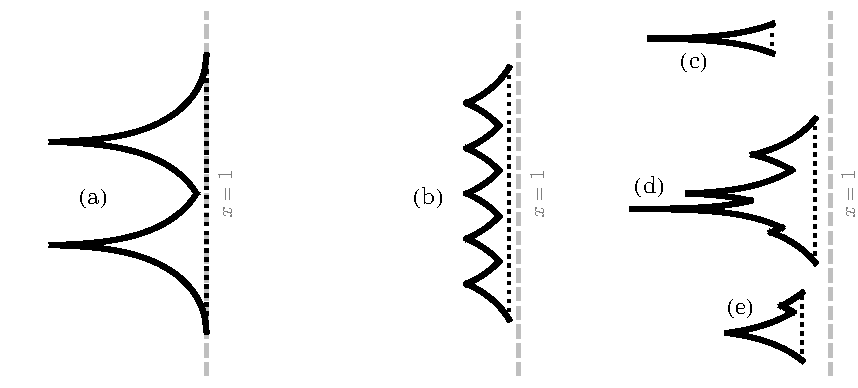
\includegraphics[width=\textwidth]{plane-domains}
  
\includegraphics[width=\textwidth]{plane-domains-legend}
  \caption{
    Five domains marked out by a radiation boundary
    and a constant-temperature boundary.
    The critical terminal curve~$x = 1$ is shown for reference.
  }
  \label{fig:plane-domains}
\end{figure}

\subsection{Domain construction}
\label{sec:cartesian.plane.domain}

Since the constructed radiation boundaries only dissipate heat,
a domain for the steady conduction--radiation BVP
will not be completely specified
until there is also a boundary to supply it.
The simplest boundary condition which can supply heat
is the Dirichlet condition~$T = \const$,
and given the form of the known solution~%
  (\ref{eq:plane-scaled-laplace-solution}),
these boundaries are simply vertical lines~$x = \const$.

An infinite number of conduction--radiation domains
may therefore be marked out
by joining a constructed radiation boundary
with an appropriate Dirichlet boundary~$x = \const$,
as in Figure~\ref{fig:plane-domains}.
Each of these domains corresponds to steady conduction in the interior,
constant temperature along the right hand side,
and thermal radiation into vacuum to the left.
Most surprising is that \emph{all} of these domains
admit the \emph{same} exact solution~(\ref{eq:plane-scaled-laplace-solution}).

Unfortunately,
the domains produced here by boundary tracing are not convex,
but \term{self-viewing}:
some of the outgoing radiation travels not to infinity,
but strikes another part of the boundary,
where it might be partially or fully absorbed.
The simple radiation boundary condition~%
  (\ref{eq:plane-scaled-radiation-boundary-condition})
does not account for this,
so while the results of this section are mathematically exact,
it is because we have an incomplete picture of the physical behaviour.

\subsection{Self-viewing radiation quantified}
\label{sec:cartesian.plane.self}

It is possible to quantify the amount of self-viewing radiation,
so that we might identify instances in which it is negligible.
In Figure~\ref{fig:plane-domains} we would expect
considerable amounts of self-viewing exchange
to occur for the domains~(a), (b), (d), and~(e)
due to the adjacent spikes.
Only for a single-spike domain such as~(c)
would we expect a small amount,
so this is the case we consider here.
While the analysis thus far has been in the $xy$-plane,
the envisaged situation consists of a three-dimensional fin
whose cross section is the domain~(c).
The analysis must necessarily be conducted in three dimensions,
as radiation can be exchanged between points on the fin surface
with different~$z$.

\begin{figure}
  \centredfigurecontent[width=0.5\textwidth]{%
    self-viewing-radiation-elements%
  }{
    Geometry of the self-viewing area elements~$\td A$ and~$\td A^\star$.
  }
\end{figure}

Consider a differential area element~$\td A$ at the local position~%
$\positionvec = x \basisvec{x} + y \basisvec{y} + z \basisvec{z}$
receiving radiation from a distant element~$\td A^\star$ at~%
$\positionvec^\star =
  x^\star \basisvec{x} + y^\star \basisvec{y} + z^\star \basisvec{z}$,
as shown in Figure~\ref{fig:self-viewing-radiation-elements}.
We denote the displacement from~$\positionvec^\star$ to~$\positionvec$ by
\begin{equation}
  \vec{d}^\star \ideq \positionvec - \positionvec^\star,
  \label{eq:self-viewing-radiation-displacement}
\end{equation}
and respectively let $\theta$ and~$\theta^\star$ be the angles
that the normals~$\normalvec$ and~$\normalvec^\star$
make with this displacement.
Writing~$T$ and~$T^\star$ for the temperatures of the two elements,
the total power emitted by~$\td A^\star$
is (in scaled terms) ${T^\star}^4 \td A^\star$.
Almost none of this will strike the element~$\td A$.
Indeed it is well known~\cite{howell-2010-thermal-radiation-heat-transfer}
that the \term{view factor} from~$\td A^\star$ to~$\td A$,
defined as the fraction of radiation which leaves~$\td A^\star$
and strikes~$\td A$,
is given by
\begin{equation}
  \textq{view factor} \ideq
    \frac{\cos\theta^\star \cos\theta \td A}{\pi {d^\star}^2},
  \label{eq:self-viewing-view-factor}
\end{equation}
where~$d^\star \ideq \norm{\vec{d}^\star}$.
It follows that the amount of radiative power arriving at~$\td A$ is
\begin{equation}
  \textq{power} \ideq
    \frac{
      {T^\star}^4 \cos\theta^\star \cos\theta \td A \td A^\star
    }{
      \pi {d^\star}^2
    }.
  \label{eq:self-viewing-power}
\end{equation}
Assuming that all of this is absorbed by~$\td A$,
we see that the radiation boundary condition~%
  (\ref{eq:plane-scaled-radiation-boundary-condition})
must be modified to
\begin{equation}
  \normalvec \dotp \del T =
    -T^4 +
    \int
      \frac{
        {T^\star}^4 \cos\theta^\star \cos\theta \td A^\star
      }{
        \pi {d^\star}^2
      }
  \label{eq:plane-scaled-radiation-boundary-condition-self-viewing}
\end{equation}
in order to account for self-viewing radiation.%
\footnote{
  Since the integral term
  in~(\ref{eq:plane-scaled-radiation-boundary-condition-self-viewing})
  is \emph{non-local},
  self-viewing radiation cannot be analysed
  using the method of boundary tracing,
  which requires a local flux condition
  of the form~(\ref{eq:flux-boundary-condition}).
}
The integral is to be taken over all elements~$\td A^\star$
which can see the element~$\td A$ at the local position~$\positionvec$.

\section{Cosinusoidal solution}
\label{sec:cartesian.cosine}

While boundary tracing as performed on
the plane-source solution~(\ref{eq:plane-laplace-solution})
did not yield convex conduction--radiation domains,
we might expect more favourable outcomes
by starting from solutions to Laplace's equation
which are not one-dimensional.
A simple class of such solutions consists of functions which are the product
of a trigonometric function in~$x$ and a hyperbolic function in~$y$.

As seen in Section~\ref{sec:cartesian.plane.domain}
we will eventually require a boundary to supply the heat being radiated away,
and from a practical point of view it is
straight-line, constant-temperature boundaries which are of interest.
Therefore in this section we consider known solutions of the form
\begin{important}{equation}
  T \ideq T_0 \roundbr*{1 - B \cos\frac{x}{L_0} \cosh\frac{y}{L_0}},
  \label{eq:cosine-laplace-solution}
\end{important}
where $T_0$~is a temperature, $L_0$~is a length scale,
and $B$~is a dimensionless constant.
The temperature is constant and takes the value~$T = T_0$
along the straight line~$x = \pi L_0/2$,
which shall ultimately serve as our heat-supplying boundary.
Physically, the constant~$B$ determines
the minimum temperature gradient along this boundary;
indeed
\begin{equation}
  \eval*{\pder{T}{x}}_{x = \pi L_0/2} = \frac{B T_0}{L_0} \cosh\frac{y}{L_0}
  \label{eq:cosine-laplace-solution-dirichlet-slope}
\end{equation}
with minimal value~$B T_0 / L_0$ at~$y = 0$,
so that solutions with a greater value of~$B$ are steeper.

\subsection{Scaling}
\label{sec:cartesian.cosine.scaling}

First the physical parameters are scaled out to the extent possible.
Using the same scalings as Section~\ref{sec:cartesian.plane.scaling},
i.e.~(\ref{eq:plane-temperature-scaling}) through~(\ref{eq:plane-del-scaling}),
the radiation boundary condition~(\ref{eq:radiation-boundary-condition})
and the known solution~(\ref{eq:cosine-laplace-solution})
become
\begin{align}
  \normalvec \dotp \scaleddel \scaled{T}
    &= -\group{c \lambda \Theta^3} \scaled{T}^4,
    \label{eq:cosine-scaled-radiation-boundary-condition-with-groups}
    \\[\tallspace]
  \scaled{T}
    &\ideq
      \group{\frac{T_0}{\Theta}}
      \roundbr*{
        1 -
          B
          \cos \roundbr*{\group{\frac{\lambda}{L_0}} \scaled{x}}
          \cosh \roundbr*{\group{\frac{\lambda}{L_0}} \scaled{y}}
      },
    \label{eq:cosine-scaled-laplace-solution-with-groups}
\end{align}
where there are two free scales, $\Theta$~(temperature) and $\lambda$~(length).
Since there are three unique dimensionless groups,
one of the groups cannot be eliminated,
and to keep the cosinusoidal terms as simple as possible
we choose the obvious scales
\begin{align}
  \Theta &= T_0,
    \label{eq:cosine-temperature-scale} \\
  \lambda &= L_0.
    \label{eq:cosine-length-scale}
\end{align}
Defining the dimensionless group
\begin{equation}
  A = \frac{1}{c L_0 {T_0}^3}.
  \label{eq:cosine-dimensionless-group}
\end{equation}
and dropping \scalingmarks,
the scaled boundary condition~%
  (\ref{eq:cosine-scaled-radiation-boundary-condition-with-groups})
and known solution~(\ref{eq:cosine-scaled-laplace-solution-with-groups})
become
\begin{important}{align}
  \normalvec \dotp \del T &= -\frac{T^4}{A},
    \label{eq:cosine-scaled-radiation-boundary-condition} \\[\tallspace]
  T &\ideq 1 - B \cos x \cosh y.
    \label{eq:cosine-scaled-laplace-solution}
\end{important}

\begin{figure}
  \centering
  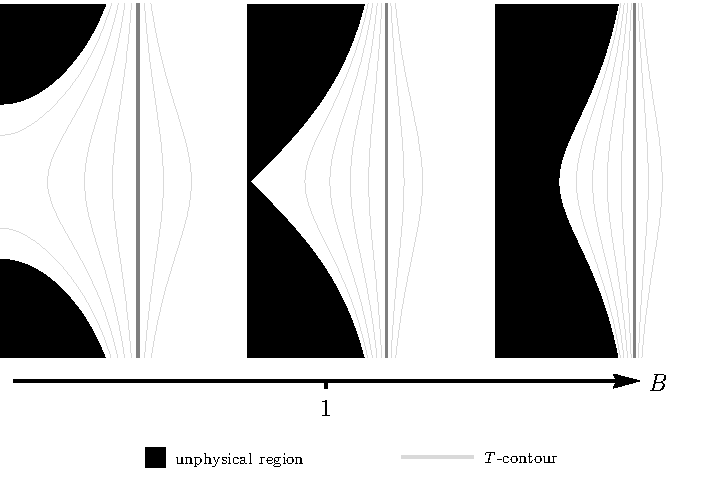
\includegraphics[width=\textwidth]{cosine-physical}
  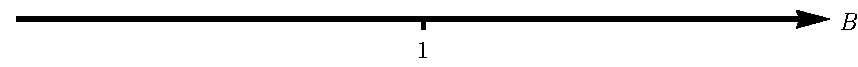
\includegraphics[width=\textwidth]{cosine-physical-arrow}
  
\includegraphics[width=\textwidth]{cosine-physical-legend}
  \caption{
    Unphysical region~$T < 0$
    for the known solution~(\ref{eq:cosine-scaled-laplace-solution}),
    as $B$~increases.
    In each plot, the left edge is~$x = 0$
    and the thick vertical line is~$x = \pi/2$,
    which is also the contour~$T = 1$.
  }
  \label{fig:cosine-physical}
\end{figure}

\subsection{Physical region}
\label{sec:cartesian.cosine.physical}

Since it is the straight-line boundary~$x = \pi/2$
which ultimately shall, in the form of a Dirichlet condition~$T = 1$,
supply the heat to be conducted and radiated away,
only the side on which~$T \le 1$ is relevant,
namely the side~$x \le \pi/2$.
Given that the known solution~(\ref{eq:cosine-scaled-laplace-solution})
is an even function of~$x$,
it also suffices to consider~$x \ge 0$ only.

Thus the region of interest
is the vertical strip~$0 \le x \le \pi/2$.
Not all of this strip is physically relevant
as only positive temperatures are admissible
in thermal radiation problems.
Since the known solution~(\ref{eq:cosine-scaled-laplace-solution})
vanishes along~$\cos x \cosh y = 1 / B$,
the geometry of the physical region~$T \ge 0$
will depend on the value of the dimensionless constant~$B$
(see Figure~\ref{fig:cosine-physical}).
The unphysical region~$T < 0$ is omitted from the remainder of the analysis,
as physically meaningful radiation boundaries cannot be found there.

\subsection{Boundary tracing equations}
\label{sec:cartesian.cosine.tracing}

In addition to only considering the physical region~$T \ge 0$,
traced boundaries will only exist within the viable domain~$\Phi \ge 0$.
For the boundary condition~%
  (\ref{eq:cosine-scaled-radiation-boundary-condition})
and known solution~(\ref{eq:cosine-scaled-laplace-solution}) at hand,
we obtain the derivatives
\begin{align}
  P &\ideq \pder{T}{x} \ideq +B \sin x \cosh y,
    \label{eq:cosine-gradient-x-component} \\[\tallspace]
  Q &\ideq \pder{T}{y} \ideq -B \cos x \sinh y,
    \label{eq:cosine-gradient-y-component}
\end{align}
the flux function
\begin{equation}
  F \ideq -\frac{(1 - B \cos x \cosh y) ^ 4}{A},
  \label{eq:cosine-flux-function}
\end{equation}
and the viability function
\begin{align*}
  \Phi
  &\ideq (\del T)^2 - F^2 \\
  &\ideq
    B^2 \roundbr*{\sin^2 x + \sinh^2 y}
      -
    \frac{(1 - B \cos x \cosh y) ^ 8}{A^2}.
    \yesnumber
    \label{eq:cosine-viability-function}
\end{align*}
The geometry of the viable domain~$\Phi \ge 0$
therefore depends on both of the dimensionless parameters~$A$ and~$B$,
as does the boundary tracing ODE~%
  (\ref{eq:tracing-ode-coordinate-parametrisation-u}),
which becomes
\begin{important}{equation}
  \tder{x}{y} = \frac{P Q \mp F \sqrt{\Phi}}{Q^2 - F^2}.
  \label{eq:cosine-tracing-ode-coordinate-parametrisation-x}
\end{important}
Given the complexity of managing more than one parameter,
we consider~$B = 1$ before examining the general case.

\subsection{Simple case (\texorpdfstring{$B = 1$}{B = 1})}
\label{sec:cartesian.cosine.simple}

\subsubsection{Viable domain}
\label{sec:cartesian.cosine.simple.viable}

In the $B = 1$~case,
the known solution~(\ref{eq:cosine-scaled-laplace-solution}) simplifies to
\begin{equation}
  T \ideq 1 - \cos x \cosh y
  \label{eq:cosine-simple-laplace-solution}
\end{equation}
and the viability function~(\ref{eq:cosine-viability-function}) reduces to
\begin{equation}
  \Phi \ideq \sin^2 x + \sinh^2 y - \frac{(1 - \cos x \cosh y) ^ 8}{A^2}.
  \label{eq:cosine-simple-viability-function}
\end{equation}
The dependence of the non-viable domain~$\Phi < 0$
on the dimensionless group~$A$
is shown in Figure~\ref{fig:cosine_simple-physical-viable}.
Radiation boundaries as produced by boundary tracing
will only be found in the white region,
which is both physical~($T \ge 0$) and viable~($\Phi \ge 0$).

The non-viable domain consists of a single%
\footnote{
  There also exist non-viable regions
  (not shown in Figure~\ref{fig:cosine_simple-physical-viable})
  which lie within the unphysical region~$T < 0$,
  but recall that the unphysical region has been omitted from the analysis
  due to physical irrelevance.
}
non-viable region which recedes towards the right as $A$~increases.
Not obvious from Figure~\ref{fig:cosine_simple-physical-viable} however
is that the boundary of this single non-viable region,
henceforth called the \term{proper} terminal curve,
only constitutes \emph{almost all} of the terminal curve.
The full terminal curve consists of the proper terminal curve
together with the origin~$(x, y) = (0, 0)$,
which is a terminal point
by virtue of being an isolated root of the equation~$\Phi = 0$.

\begin{figure}
  \centering
  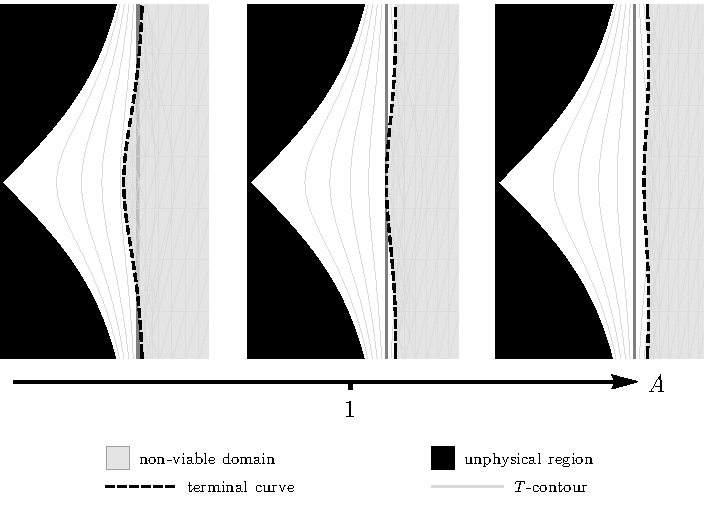
\includegraphics[width=\textwidth]{cosine_simple-physical-viable}
  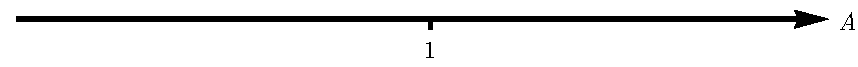
\includegraphics[width=\textwidth]{cosine_simple-physical-viable-arrow}
  
\includegraphics[width=\textwidth]{cosine_simple-physical-viable-legend}
  \caption{
    Non-viable domain~$\Phi < 0$
    for the known solution~(\ref{eq:cosine-simple-laplace-solution})
    and viability function~(\ref{eq:cosine-simple-viability-function}),
    as $A$~increases.
    In each plot, the left edge is~$x = 0$
    and the thick vertical line is~$x = \pi/2$,
    which is also the contour~$T = 1$.
  }
  \label{fig:cosine_simple-physical-viable}
\end{figure}

\subsubsection{Boundary tracing}
\label{sec:cartesian.cosine.simple.tracing}

The tracing ODE~%
  (\ref{eq:cosine-tracing-ode-coordinate-parametrisation-x})
cannot be integrated analytically,
so the traced boundaries are determined numerically.
In doing so, the parametrisation~$x = x (y)$
is unable to handle traced boundaries which are locally horizontal;
such difficulty is avoided by instead using the arc-length parametrisation~%
  (\ref{eq:tracing-ode-arc-length-parametrisation-u})
\&~(\ref{eq:tracing-ode-arc-length-parametrisation-v}),
which for Cartesian coordinates reduces to
\begin{align}
  \tder{x}{s} &= \frac{-Q F \pm P \sqrt{\Phi}}{(\del T)^2},
    \label{eq:cosine-tracing-ode-arc-length-parametrisation-x} \\[\tallspace]
  \tder{y}{s} &= \frac{+P F \pm Q \sqrt{\Phi}}{(\del T)^2}.
    \label{eq:cosine-tracing-ode-arc-length-parametrisation-y}
\end{align}
Two branches of traced boundaries are obtained
by integrating forward
from starting points within the region
both physical~($T \ge 0$) and viable~($\Phi \ge 0$).
The resulting curves (Figure~\ref{fig:cosine_simple-traced-boundaries})
are boundaries along which the radiation boundary condition~%
  (\ref{eq:cosine-scaled-radiation-boundary-condition})
is satisfied.
For the correct boundary orientation,
note that the temperature~$T$ is an increasing function of~$x$;
it follows that the interior lies to the right of each boundary curve,
with heat being lost by radiation to the left.

\begin{figure}
  \centredfigurecontent[width=0.42\textwidth]{%
    cosine_simple-traced-boundaries%
  }{
    Traced boundaries for~$A = 0.5$,
    obtained by integrating
    (\ref{eq:cosine-tracing-ode-arc-length-parametrisation-x})
    \&~(\ref{eq:cosine-tracing-ode-arc-length-parametrisation-y}).
  }
\end{figure}

By patching together the traced boundaries,
an unlimited number of radiation boundaries may be constructed.
However, almost all such constructions are non-convex
(see Figure~\ref{fig:cosine_simple-traced-boundaries-patched-spiky}).
At any point \emph{strictly} within the viable domain,
i.e.~$\Phi > 0$,
the two traced boundaries through it will cross at a non-zero angle,
and patching these two boundaries together
inevitably results in a spike made of non-convex curves.
As noted already in Section~\ref{sec:cartesian.plane.domain},
self-viewing radiation is not accounted for
by the simple radiation boundary condition~%
  (\ref{eq:cosine-scaled-radiation-boundary-condition}),
and so the non-convex constructions are all invalid.

\begin{figure}
  \newcommand*{\subfigurewidth}{0.36\textwidth}
  \centering
  \hspace*{\fill}
  \begin{subfigure}[t]{\subfigurewidth}
    \centredfigurecontent{cosine_simple-traced-boundaries-patched-spiky}{%
      Spiky non-convex boundary
    }
  \end{subfigure}
    \hfill
  \begin{subfigure}[t]{\subfigurewidth}
    \centredfigurecontent{cosine_simple-traced-boundaries-patched-smooth}{%
      Smooth candidate boundary
    }
  \end{subfigure}
  \hspace*{\fill}
  \caption{
    Radiation boundaries~\figurestyle{thick black} patched together
    using traced boundaries~\figurestyle{grey}.
  }
  \label{fig:cosine_simple-traced-boundaries-patched}
\end{figure}

\begin{figure}
  \centredfigurecontent[width=0.63\textwidth]{%
    cosine_simple-terminal-points%
  }{
    $T$-contours which intersect the proper terminal curve~$\Phi = 0$,
    which is the border of the non-viable domain~$\Phi < 0$.
    The horizontal scale is exaggerated.
  }
\end{figure}

To avoid the non-convex spikes,
the join must occur at a point along the terminal curve~$\Phi = 0$.
Specifically this point must not be an ordinary terminal point,
at which the two traced boundaries being patched
would form a cusp with inconsistent boundary orientation
(see Section~\ref{sec:introduction.tracing}).
Instead the join must occur at a critical terminal point;
we recall that this is a point along the terminal curve
for which the local $T$-contour touches the terminal curve~$\Phi = 0$
tangentially (rather than crossing at a non-zero angle).

Now in the present situation,
the full terminal curve consists of
an isolated terminal point at the origin
in union with the proper terminal curve
(which is the boundary of the non-viable region
visible in Figure~\ref{fig:cosine_simple-physical-viable}).
The terminal point at the origin is already notable due to its isolation,
but even more remarkable is that the local $T$-contour~($T = 0$)
looks like~$y = \pm x$.
One therefore wonders:
  are the local $T$-contour (whose tangent is indeterminate)
  and the local portion of the terminal curve (which is just a point)
  \emph{tangential}, and therefore,
  is the origin a \emph{critical} terminal point?
While the tangency is debatable,
the answer to the criticality question ought to be yes
on account of the actual behaviour:
two traced boundaries pass through the origin
(see Figure~\ref{fig:cosine_simple-traced-boundaries})
as if it were a hyperbolic critical terminal point,
with $y = 0$~as the common tangent.
Unfortunately the pair of traced boundaries forms a non-convex spike,
which is of no use here.

With the origin ruled out,
it remains to consider the proper terminal curve.
Figure~\ref{fig:cosine_simple-terminal-points} shows that in the present case,
all points along the proper terminal curve are ordinary
except for a single critical terminal point~$(x, y) = (x_0, 0)$
at the intersection of the proper terminal curve
and the horizontal axis~$y = 0$.
Algebraically, $x_0$~is the positive%
\footnote{
  The trivial solution~$x = 0$
  corresponds to the isolated terminal point at the origin,
  which we have just dismissed.
}
solution to
\begin{equation}
  \eval[\textsize]{\Phi}_{y=0}
  \ideq \roundbr*{1 - \cos^2 x} - \frac{(1 - \cos x)^8}{A^2}
  = 0,
  \label{eq:cosine-simple-critical-terminal-point-x}
\end{equation}
a polynomial equation in~$\cos x$.
Furthermore, the local $T$-contour through~$(x_0, 0)$
lies on the viable side of the proper terminal curve;
therefore the critical terminal point~$(x_0, 0)$ is of hyperbolic type,
with two traced boundaries passing through it smoothly.
By patching together the portions which lie to the right of~$(x_0, 0)$,
a single spike-free radiation boundary can be constructed
as shown in Figure~\ref{fig:cosine_simple-traced-boundaries-patched-smooth};
this boundary shall be referred to as the \term{candidate boundary}.
It is interesting to note that
the candidate boundary and the proper terminal curve
are virtually indistinguishable;
despite only touching each other at the critical terminal point~$(x_0, 0)$,
the former asymptotically approaches the latter travelling away from~$y = 0$.

\subsubsection{Convexity}
\label{sec:cartesian.cosine.simple.convexity}

The choice of the candidate boundary over all other boundary patchings
is a necessary but not sufficient condition for convexity.
While the candidate boundary is convex at~$(x_0, 0)$,
it will eventually inflect
at some~$(x, y) = (x_\infl, \pm y_\infl)$ depending on~$A$,
and become concave.

Recalling the goal of constructing domains
corresponding to a conduction--radiation BVP\@,
a \term{candidate domain} is demarcated by using
the candidate boundary as the radiation boundary
and the straight line~$x = \pi/2$
as a constant-temperature heat-supplying boundary.
The continuum of candidate domains (for~$0 < A < 1$)\footnote{
  At~$A = 1$ the candidate boundary touches the line~$x = \pi/2$,
  and the candidate domain shrinks to a point.
}
is shown in Figure~\ref{fig:cosine_simple-candidate-domains};
each domain is shaped like a thin lens,
corresponding to steady conduction in its interior,
thermal radiation along the curved boundary to the left,
and constant temperature~$T = 1$ along the straight boundary on the right.
The domain will be valid if the curved boundary
(which is a portion of the corresponding candidate boundary)
is convex, or equivalently,
if the first inflection of the corresponding candidate boundary
occurs at abscissa~$x_\infl \ge \pi/2$.

\begin{figure}
  \newcommand*{\legendtrimwidth}{0.1\textwidth}
  \newcommand*{\legendoffsetheight}{0.36\textwidth}
  \centering
  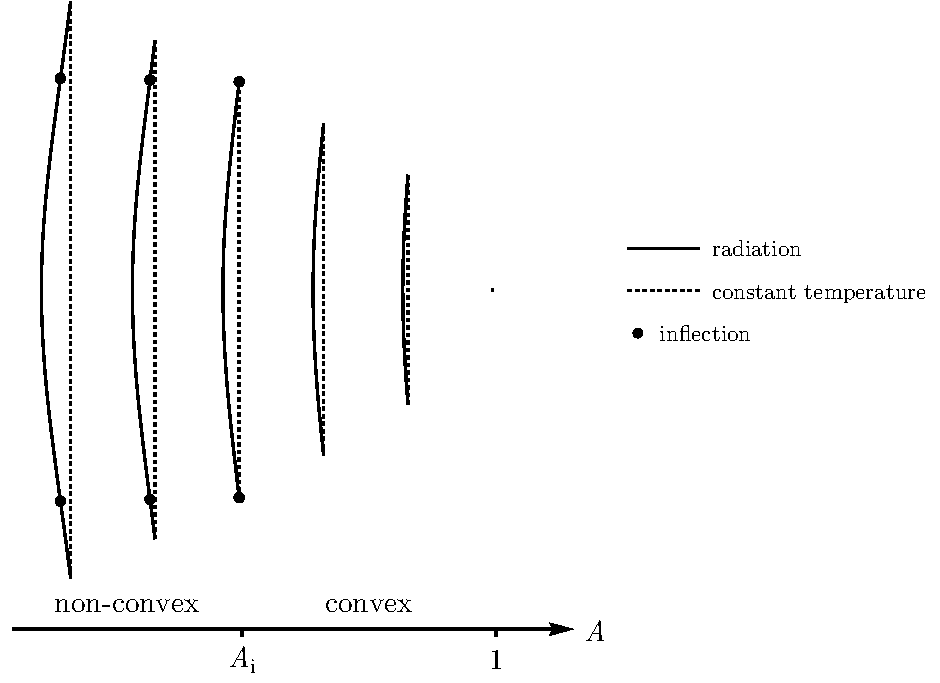
\includegraphics[width=0.6\textwidth]{cosine_simple-candidate-domains}
  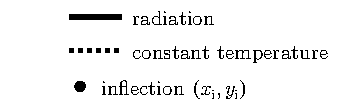
\includegraphics[
    width={0.4\textwidth-\legendtrimwidth},
    trim={\legendtrimwidth} {-\legendoffsetheight} 0 0,
  ]{cosine_simple-candidate-domains-legend}
  \caption{
    Candidate domains marked out by a radiation boundary
    and the constant-temperature boundary~$x = \pi/2$,
    as $A$~increases.
    Points of inflection are shown for reference.
  }
  \label{fig:cosine_simple-candidate-domains}
\end{figure}

The critical value~$A = A_\infl$
(where the candidate domain changes from invalid to valid)
is that for which the first inflection occurs at precisely~$x_\infl = \pi/2$.
Given that the candidate boundary is never horizontal,
$A_\infl$~is best sought using the coordinate parametrisation~$x = x (y)$
for the candidate boundary.
In Cartesian coordinates, points of inflection
are simply given by zero-crossings in the second derivative,
or, using primes for $y$-differentiation, $x''$.
Differentiating the first derivative~%
  (\ref{eq:cosine-tracing-ode-coordinate-parametrisation-x})
gives
\begin{equation}
  x'' = \tder{}{y} \roundbr*{\frac{P Q \mp F \sqrt{\Phi}}{Q^2 - F^2}},
  \label{eq:acceleration-traced-boundary-cartesian-by-y}
\end{equation}
whose right hand side may be reduced to a function purely of~$x$ and~$y$
by applying~(\ref{eq:cosine-tracing-ode-coordinate-parametrisation-x})
once more to eliminate the first derivatives.
Substituting~$x = x_\infl = \pi/2$, this becomes
\begin{equation}
  \eval[\textsize]{x''}_{x=\pi/2} =
    \frac{A^2 C}{\sqrt{A^2 C^2 - 1}}
    \squarebr*{
      2 S - \roundbr*{1 + S^2} \roundbr*{A^2 S + 4 \sqrt{A^2 (1 + S^2) - 1}}
    },
  \label{eq:%
    cosine-simple-traced-boundary-acceleration-cartesian-by-y-inflection%
  }
\end{equation}
where $C \ideq \cosh y$ and~$S \ideq \sinh y$.
Only the square-bracketed factor can change sign,
and an analysis shows that for~$0 < A < 1$,
this factor has a unique zero-crossing~$S = S_\infl (A)$.
The would-be $y$-coordinate of inflection for a given~$A$ is therefore
\begin{equation}
  y = y_\infl (A) = \sinh^{-1} \roundbr[\bulkysize]{S_\infl (A)}.
  \label{eq:cosine-simple-traced-boundary-y-would-be-inflection}
\end{equation}
Since the inflection is supposed to occur at~$x_\infl = \pi/2$,
the critical value~$A = A_\infl$ is the solution to
\begin{equation}
  x \roundbr[\bulkysize]{y_\infl (A)} = \pi/2,
  \label{eq:cosine-simple-traced-boundary-a-inflection-equation}
\end{equation}
whose left hand side is the coordinate parametrisation~$x = x (y)$
evaluated at the would-be $y$-coordinate~%
  (\ref{eq:cosine-simple-traced-boundary-y-would-be-inflection}).
Using the bisection algorithm we obtain the root
\begin{equation}
  A_\infl = 0.79718,
  \label{eq:cosine-simple-traced-boundary-a-inflection}
\end{equation}
and therefore the lens-like candidate domain for a given~$A$ is convex
if and only if
\begin{equation}
  A_\infl \le A < 1.
  \label{eq:cosine-simple-traced-boundary-convex-a-interval}
\end{equation}

\subsection{General case (\texorpdfstring{$B$~arbitrary}{B arbitrary})}
\label{sec:cartesian.cosine.general}

\subsubsection{Viable domain}
\label{sec:cartesian.cosine.general.viable}

In the general case the dimensionless group~$B$ may also be varied,
and altogether the parameter space~$(A, B)$ is two-dimensional.
Two degrees of freedom is too many to manage,
and the behaviour of the viable domain is best understood
by fixing~$A$ and varying~$B$.

\begin{figure}
  \newcommand*{\legendoffsetheight}{0.1\textwidth}
  \centering
  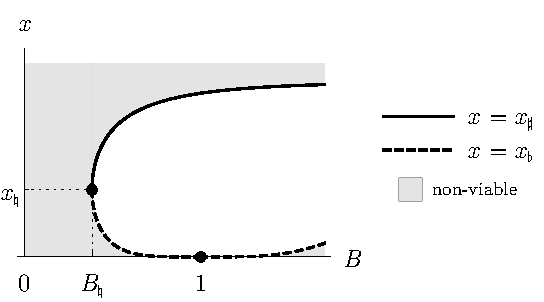
\includegraphics[width=0.45\textwidth]{cosine_general-critical}
  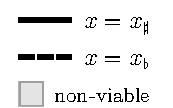
\includegraphics[
    width=0.2\textwidth,
    trim=0 {-\legendoffsetheight} 0 0,
  ]{cosine_general-critical-legend}
  \caption{
    Terminal points along the $x$-axis, as $B$~increases with $A$~fixed.
  }
  \label{fig:cosine_general-critical}
\end{figure}

Of particular interest are the terminal points along the $x$-axis;
these are necessarily critical terminal points
because the local $T$-contour and the terminal curve~$\Phi = 0$
both cross the $x$-axis vertically
(as $T$ and~$\Phi$ are both even functions of~$y$),
and are therefore tangential.
Algebraically these terminal points are given by the roots of
\begin{equation}
  \eval[\textsize]{\Phi}_{y=0}
  \ideq B^2 \sin^2 x - \frac{(1 - B \cos x)^8}{A^2}
  = 0,
  \label{eq:cosine-general-critical-terminal-point-x}
\end{equation}
which are shown in Figure~\ref{fig:cosine_general-critical}.
For sufficiently small~$B$,
there are no roots and the entire $x$-axis is non-viable,
until a single root~$x = x_\nat (A)$ appears at~$B = B_\nat (A)$.
As $B$~increases past this transitional value,
the root splits into two roots, $x = x_\flat (A, B)$ and~$x = x_\sharp (A, B)$.
At~$B = 1$, the lesser root~$x_\flat$ vanishes,
before becoming positive again but unphysical for~$B > 1$.
In terms of the viable domain, this translates into five cases
(Figure~\ref{fig:cosine_general-physical-viable}):
\begin{enumerate}
  \item
    \label{itm:cartesian.cosine.general.regimes.gentle}
    \term{Gentle regime}, $B < B_\nat (A)$:
    The non-viable domain completely envelopes the $x$-axis,
    dividing the viable domain into two halves.
    Two hyperbolic critical terminal points exist along the $y$-axis
    at~$(x, y) = (0, \pm y_0)$.
  \item
    \label{itm:cartesian.cosine.general.regimes.gentle-to-fair}
    \term{Gentle-to-fair transition}, $B = B_\nat (A)$:
    The two viable regions pinch together at~$(x, y) = (x_\nat, 0)$,
    a critical terminal point of hyperbolic type.%
    \footnote{
      Here the local $T$-contour crosses the $x$-axis vertically
      while the terminal curve~$\Phi = 0$ has indeterminate tangent
      (being the location of a self-intersection).
      While the tangency is again debatable,
      two traced boundaries pass through vertically
      as if the vertical line~$x = x_\nat$ were the common tangent.
    }
    The non-viable domain now consists of two disjoint regions.
  \item
    \label{itm:cartesian.cosine.general.regimes.fair}
    \term{Fair regime}, $B_\nat (A) < B < 1$:
    The two non-viable regions are sundered further apart
    by a growing viable tract along the $x$-axis,
    with $(x_\nat, 0)$~splitting into the two
    hyperbolic critical terminal points~$(x_\flat, 0)$ and~$(x_\sharp, 0)$.
  \item
    \label{itm:cartesian.cosine.general.regimes.fair-to-steep}
    \term{Fair-to-steep transition}, $B = 1$:
    This is the simple case
    of Section~\ref{sec:cartesian.cosine.general.viable};
    the hyperbolic critical terminal point~$(x_\sharp, 0)$
    is what was formerly called~$(x_0, 0)$.
    The smaller non-viable region of the fair regime
    has shrunken to nothingness,
    and the critical terminal points~$(0, \pm y_0)$ and~$(x_\flat, 0)$
    have merged together
    to form the isolated critical terminal point at the origin.
  \item
    \label{itm:cartesian.cosine.general.regimes.steep}
    \term{Steep regime}, $B > 1$:
    The smaller non-viable region
    reappears but is overrun by the growing unphysical region.
    The terminal points~$(0, \pm y_0)$ (if they exist)
    and~$(x_\flat, 0)$ all lie in the unphysical region
    and are therefore irrelevant,
    leaving a single hyperbolic critical terminal point~$(x_\sharp, 0)$.
\end{enumerate}

\subsubsection{Boundary tracing}
\label{sec:cartesian.cosine.general.tracing}

An exhaustive treatment cannot be given here
due to the complex dependence
of the known solution~$T$ and the viability function~$\Phi$
on both~$A$ and~$B$.
Nevertheless, broad statements can be made.

\begin{figure}
  \centering
  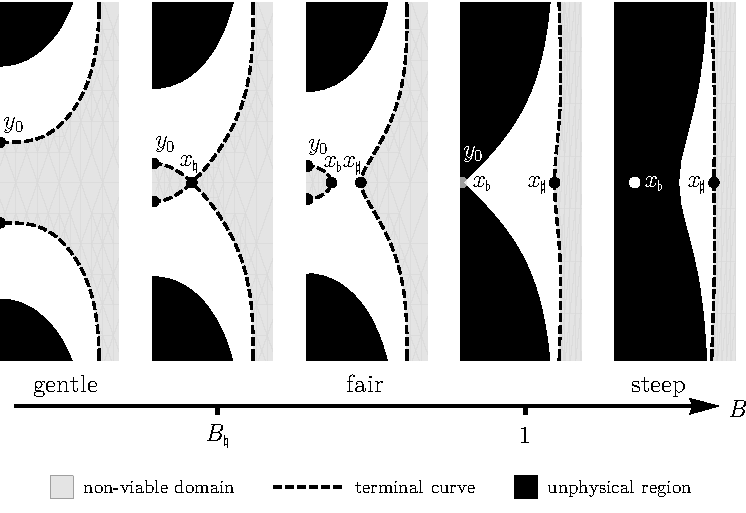
\includegraphics[width=\textwidth]{cosine_general-physical-viable}
  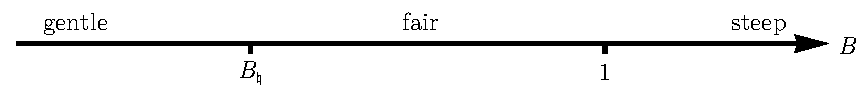
\includegraphics[width=\textwidth]{cosine_general-physical-viable-arrow}
  
\includegraphics[width=\textwidth]{cosine_general-physical-viable-legend}
  \caption{
    Non-viable domain~$\Phi < 0$ and critical terminal points
    for the known solution~(\ref{eq:cosine-scaled-laplace-solution})
    and viability function~(\ref{eq:cosine-viability-function}),
    as $B$~increases with $A$~fixed.
    In each plot, the left edge is~$x = 0$ and the right edge is~$x = 2$.
  }
  \label{fig:cosine_general-physical-viable}
\end{figure}

In Case~\ref{itm:cartesian.cosine.general.regimes.gentle} (gentle regime)
only non-convex spikes can be formed
by patching together traced boundaries,
even at the critical terminal points~$(0, \pm y_0)$ along the $y$-axis.
Case~\ref{itm:cartesian.cosine.general.regimes.fair-to-steep}
  (fair-to-steep transition)
is the simple $B = 1$~case which we have already analysed
in Section~\ref{sec:cartesian.cosine.general.viable};
recall that a conduction--radiation domain in the shape of a convex lens
can be produced for each~$A$ in the interval~%
  (\ref{eq:cosine-simple-traced-boundary-convex-a-interval})
by using the traced boundaries which pass through~$(x_0, 0)$
(now called~$(x_\sharp, 0)$).
The situation in
Case~\ref{itm:cartesian.cosine.general.regimes.steep} (steep regime)
is very similar,
but the convex lens shapes which can be produced
are even thinner than those of
Case~\ref{itm:cartesian.cosine.general.regimes.fair-to-steep}.

This leaves
Case~\ref{itm:cartesian.cosine.general.regimes.gentle-to-fair}
  (gentle-to-fair transition)
and
Case~\ref{itm:cartesian.cosine.general.regimes.fair} (fair regime),
the former of which need not be treated separately
since it is effectively a degenerate version of the latter
(with~$x_\flat = x_\sharp$).
In the same manner as a spike-free candidate boundary
was constructed through~$(x_0, 0)$
in Section~\ref{sec:cartesian.cosine.general.viable},
so may candidate boundaries be constructed
through the hyperbolic critical terminal points~%
  $(x_\flat, 0)$ and~$(x_\sharp, 0)$.
Again we can form lens-shaped candidate domains,
and these will be convex for sufficiently well-chosen~$A$ and~$B$.

Much more interesting however is the existence
in Case~\ref{itm:cartesian.cosine.general.regimes.fair} (fair regime)
of convex conduction--radiation domains
which are \emph{not} shaped as lenses.
We cannot perform a general analysis here
due to the complex dependence of the curvature on~$A$ and~$B$,
so we look at the illustrative example~$(A, B) = (12, 0.082506)$.
Figure~\ref{fig:cosine_general-traced-boundaries-convex}
shows (among other features) the frontiers of inflection
for the two branches of traced boundaries,
which we obtain by computing the zero-contours of the second derivative~%
  (\ref{eq:acceleration-traced-boundary-cartesian-by-y})
using numerical integration.
Only the portions of traced boundary which lie
convex side of the inflection frontiers
will be valid as radiation boundaries.
Since the end is to construct a domain
with the straight line contour~$x = \pi/2$
serving as the constant-temperature boundary,
we immediately discard any convex portion of traced boundary
which does not reach~$x = \pi/2$.
Of the remaining convex portions,
those which do not reach the $x$-axis~($y = 0$)
are unable to join up with a convex portion of the opposite branch
(which is necessary to form a complete domain boundary);
discarding those also leaves the convex portions of traced boundary
shown in Figure~\ref{fig:cosine_general-traced-boundaries-convex}.

\begin{figure}
  \newcommand*{\subfigurewidth}{0.45\textwidth}
  \centering
  \includegraphics[width=\textwidth, trim=0 -10 0 0]%
    {cosine_general-asymmetric-construction-legend}
  \hspace*{\fill}
  \begin{subfigure}[t]{\subfigurewidth}
    \centredfigurecontent{cosine_general-traced-boundaries-convex}{%
      Convex portions of the two branches of traced boundaries
      which reach both the constant-temperature boundary~$x = \pi/2$
      and the $x$-axis.
    }
  \end{subfigure}
  \hfill
  \begin{subfigure}[t]{\subfigurewidth}
    \centredfigurecontent{cosine_general-asymmetric_domain}{%
      An asymmetric domain marked out by a radiation boundary
      and the constant-temperature boundary~$x = \pi/2$.
    }
  \end{subfigure}
  \hspace*{\fill}
  \caption{
    Constructing an asymmetric conduction--radiation domain
    for~$(A, B) = (12, 0.082506)$ (fair regime).
  }
  \label{fig:cosine_general-asymmetric-construction}
\end{figure}

The smooth traced boundary through the critical terminal point~$(x_\sharp, 0)$
may be used to construct the familiar lens-shaped domain.
The remaining convex portions of traced boundary
shown in Figure~\ref{fig:cosine_general-traced-boundaries-convex}
can be used to construct conduction--radiation domains
which are not lens-shaped, including asymmetric domains
(Figure~\ref{fig:cosine_general-asymmetric_domain});
simply take two intersecting traced boundaries
(one from the lower branch and one from the upper)
which are not reflections of each other,
and trim them at their intersection
and where they meet the constant-temperature boundary~$x = \pi/2$.
It is most remarkable that
\emph{any} conduction--radiation domain constructed in this manner
will admit the very same exact solution~%
  (\ref{eq:cosine-scaled-laplace-solution}).

\subsection{Numerical verification}
\label{sec:cartesian.cosine.verification}

The validity of any convex domain constructed
in Sections~\ref{sec:cartesian.cosine.simple.convexity}
and~\ref{sec:cartesian.cosine.general.tracing}
may be tested by numerically solving the conduction--radiation BVP
in that domain and comparing the result
to the exact solution~(\ref{eq:cosine-scaled-laplace-solution}).
To do this we use \software{Mathematica~12},
whose finite elements package~\code{NDSolve\`{}FEM\`{}}
has built-in capabilities for mesh generation and for solving nonlinear BVPs.

\begin{figure}
  \newcommand*{\legendoffsetheight}{0.1\textwidth}
  \centering
  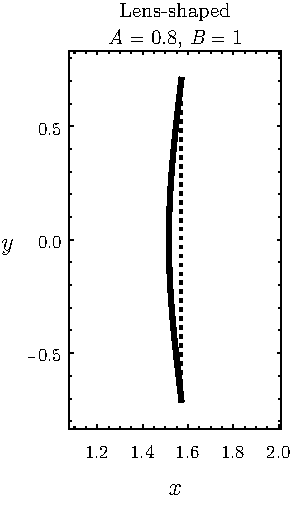
\includegraphics[height=0.6\textwidth]{cosine-verification-lens-domain}
  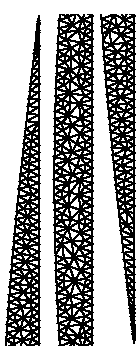
\includegraphics[
    width=0.16\textwidth,
    trim=0 {-\legendoffsetheight} 0 0,
  ]{cosine-verification-lens-mesh}
  \hfill
  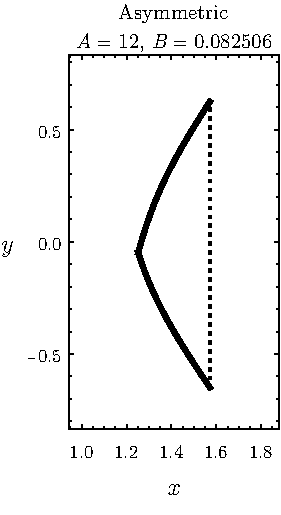
\includegraphics[height=0.6\textwidth]{cosine-verification-asymmetric-domain}
  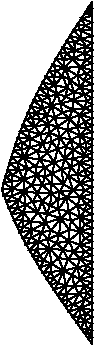
\includegraphics[
    width=0.11\textwidth,
    trim=0 {-\legendoffsetheight} 0 0,
  ]{cosine-verification-asymmetric-mesh}
  
\includegraphics[width=\textwidth]{cosine-verification-legend}
  \caption{
    Selected domains and finite element meshes for numerical verification.
  }
  \label{fig:cosine-verification-domain-meshes}
\end{figure}

Figure~\ref{fig:cosine-verification-domain-meshes}
shows the two selected test domains:
for the simple case~($B = 1$),
this is the lens-shaped domain with~$A = 0.8$,
and for the general case~($B$~arbitrary),
the asymmetric domain constructed
in Figure~\ref{fig:cosine_general-asymmetric_domain}.
Each domain is discretised into an unstructured triangular mesh
with around 500~elements.

Laplace's equation~(\ref{eq:laplace-steady-conduction}) is then solved,
with the radiation condition~%
  (\ref{eq:cosine-scaled-radiation-boundary-condition})
applied along the radiation boundary
and the Dirichlet condition~$T = 1$ applied
along the constant-temperature boundary~$x = \pi/2$.
The agreement between the resulting numerical solutions
and the exact solution~(\ref{eq:cosine-scaled-laplace-solution})
is excellent;
in both cases the relative error is strictly less than~$\SI{0.06}{\percent}$
throughout all vertices of the mesh,
and we can therefore be completely confident
in the validity of the boundary tracing procedure.

\section{Summary}
\label{sec:cartesian.summary}

In this chapter we have applied the method of boundary tracing
for the conduction--radiation problem in Cartesian coordinates.
Starting from the simplest possible solution,
namely the one-dimensional solution~(\ref{eq:plane-laplace-solution}),
we have produced
a family of hypergeometric traced boundaries
with translational symmetry in~$y$.
By construction
the radiation condition~(\ref{eq:radiation-boundary-condition})
holds exactly along these boundaries,
and they may be patched together
to form a broad variety of radiation boundaries.
Unfortunately these boundaries are physically invalid
because they are not convex,
and the boundary condition~(\ref{eq:radiation-boundary-condition})
does not account for self-viewing radiation.

A more favourable outcome might be expected
by starting from a solution to Laplace's equation
which is not one-dimensional.
The conduction--radiation problem requires a heat source,
and since it is straight-line, constant-temperature boundaries
which are of physical interest,
we have chosen the cosinusoidal solution~(\ref{eq:cosine-laplace-solution}),
which has the straight-line contour~$x = \pi L_0/2$.
In the simple case~($B = 1$)
we have seen that a lens-shaped domain can be produced
which is convex for certain values of the dimensionless group~$A$,
while for the more complicated general case~($B$~arbitrary)
we have demonstrated the construction of an asymmetric domain
from convex portions of the traced boundaries.
Finally the validity of the domains produced has been confirmed,
by comparing numerical solutions to the conduction--radiation BVP
(obtained using the finite element method)
with the exact cosinusoidal solution
unto which boundary tracing was applied.

\chapter{Polar coordinates}
\label{ch:polar}

In this chapter,
we apply boundary tracing to the conduction--radiation problem
using the fundamental line-source solution
as the known solution to
Laplace's equation~(\ref{eq:laplace-steady-conduction}).
As in Chapter~\ref{ch:cartesian},
traced boundaries are sought along which
the radiation condition~(\ref{eq:radiation-boundary-condition})
is satisfied.
The convex portions of these traced boundaries are then used
to construct conduction--radiation domains
which admit the same line-source solution.

\section{Line-source solution}
\label{sec:polar.line}

First we establish the known solution and the appropriate scaling.

The line-source solution
to Laplace's equation~(\ref{eq:laplace-steady-conduction})
is usually encountered in electrostatics,
where it represents the potential of a line charge,
logarithmic in the cylindrical radius~$r \ideq \sqrt{x^2 + y^2}$.
In the context of steady conduction,
the only dimensionally consistent form for this is
\begin{important}{equation}
  T \ideq T_0 \log \roundbr*{\frac{r_0}{r}}
  \label{eq:line-laplace-solution}
\end{important}
for some temperature~$T_0$ and radius~$r_0$.%
\footnote{
  Whereas the power law~$T = C r^n$ is scale-invariant,
  requiring only \emph{one} constant~$C$,
  the logarithm does not possess this property;
  separate constants are required for~$T$ and for~$r$.
}
Note that the region~$r > r_0$ is unphysical,
since there the temperature is negative.

Clearly it is sensible to work in the usual polar coordinates~$(r, \phi)$
given by the transformation
\begin{align}
  x &\ideq r \cos\phi, \label{eq:x-transformation-polar} \\
  y &\ideq r \sin\phi, \label{eq:y-transformation-polar}
\end{align}
with scale factors
\begin{align}
  \scalefac[r] &\ideq 1, \label{eq:r-scale-factor-polar} \\
  \scalefac[\phi] &\ideq r. \label{eq:phi-scale-factor-polar}
\end{align}

\subsection{Scaling}
\label{sec:polar.line.scaling}

While the known solution~(\ref{eq:line-laplace-solution})
already has intrinsic temperature and length scales $T_0$ and~$r_0$,
the final scaling should also account for
the radiation boundary condition~(\ref{eq:radiation-boundary-condition}).

Let
\begin{align}
  \scaled{T} &\ideq T / \Theta, \label{eq:line-scaled-temperature} \\
  \scaled{r} &\ideq r / \varrho, \label{eq:line-scaled-r}
\end{align}
with~$\Theta$ and~$\varrho$ to be chosen later.
Noting that
\begin{equation}
  \scaleddel \ideq \varrho \del,
  \label{eq:line-scaled-del}
\end{equation}
the radiation boundary condition~(\ref{eq:radiation-boundary-condition})
and the known solution~(\ref{eq:line-laplace-solution})
become
\begin{align}
  \normalvec \dotp \scaleddel \scaled{T}
    &= -\group{c \varrho \Theta^3} \scaled{T}^4,
    \label{eq:line-scaled-radiation-boundary-condition-with-groups}
    \\[\tallspace]
  \scaled{T}
    &\ideq
      \group{\frac{T_0}{\Theta}}
      \log \roundbr*{\frac{\group{r_0 / \varrho}}{\scaled{r}}}.
    \label{eq:line-scaled-laplace-solution-with-groups}
\end{align}
There are three dimensionless groups
but only two free scales~$\Theta$ and~$\varrho$,
so one of the groups cannot be eliminated.
To keep the logarithm as simple as possible,
we put
\begin{align}
  \Theta &= T_0,
    \label{eq:line-temperature-scale} \\
  \varrho &= r_0,
    \label{eq:line-length-scale}
\end{align}
and define the dimensionless group
\begin{equation}
  A = \frac{1}{c r_0 {T_0}^3}.
  \label{eq:line-dimensionless-group}
\end{equation}
Dropping \scalingmarks, the scaled boundary condition~%
  (\ref{eq:line-scaled-radiation-boundary-condition-with-groups})
and known solution~(\ref{eq:line-scaled-laplace-solution-with-groups})
become
\begin{important}{align}
  \normalvec \dotp \del T &= -\frac{T^4}{A},
    \label{eq:line-scaled-radiation-boundary-condition} \\[\tallspace]
  T &\ideq -\log r.
    \label{eq:line-scaled-laplace-solution}
\end{important}
Note that the scale factors~%
  (\ref{eq:r-scale-factor-polar}) and~(\ref{eq:phi-scale-factor-polar})
are unchanged in form by the scaling.

\section{Viable domain}
\label{sec:polar.viable}

Next we determine the geometry of the viable domain,
the region in which traced boundaries exist.

Comparing the radiation condition~%
  (\ref{eq:line-scaled-radiation-boundary-condition})
to the generic flux condition~(\ref{eq:flux-boundary-condition}),
it follows that the flux function is
\begin{align*}
  F
  &\ideq -\frac{T^4}{A} \\[\tallspace]
  &\ideq -\frac{\log^4 r}{A}.
    \yesnumber
    \label{eq:line-flux-function}
\end{align*}
The radial and azimuthal components of the gradient~$\del T$ are
\begin{align}
  P &\ideq \pder{T}{r} \ideq -\frac{1}{r},
    \label{eq:line-gradient-u-component} \\[\tallspace]
  Q &\ideq \frac{\pd T}{r \pd\phi} \ideq 0,
    \label{eq:line-gradient-v-component}
\end{align}
and so the viability function is given by
\begin{align*}
  \Phi
  &\ideq (\del T)^2 - F^2 \\[\tallspace]
  &\ideq \frac{1}{r^2} - \frac{\log^8 r}{A^2} \\[\tallspace]
  &\ideq \frac{A^2 - \psi^2}{A^2 r^2},
    \yesnumber
    \label{eq:line-viability-function}
\end{align*}
where $\psi$~is the auxiliary function
\begin{equation}
  \psi (r) \ideq r \log^4 r.
  \label{eq:line-auxiliary-function}
\end{equation}
The viable domain is therefore the region~$\psi (r) \le A$.

\subsection{Auxiliary function properties}
\label{sec:polar.viable.psi}

\begin{figure}
  \centredfigurecontent[width=0.6\textwidth]{%
    line-auxiliary-function%
  }{
    Auxiliary function~(\ref{eq:line-auxiliary-function}).
  }
\end{figure}

Since the region~$r > 1$ is unphysical
(corresponding to negative temperature),
it is only necessary to consider~$0 \le r \le 1$.
On this interval, $\psi$~is positive
except at the endpoints~$r = 0$ and~$r = 1$, where it vanishes.
Observing that the slope
\begin{equation}
  \tder{\psi}{r} \ideq (4 + \log r) \log^3 r
  \label{eq:line-psi-r-derivative}
\end{equation}
changes sign from positive to negative
as $r$~increases through~$\ee^{-4}$,
it follows that $\psi$~has a single maximum on~$0 \le r \le 1$ at
\begin{equation}
  r = r_\nat = \ee^{-4} = 0.01832,
  \label{eq:line-r-natural}
\end{equation}
where it takes the maximal value
\begin{equation}
  \psi
  = A_\nat
  = \psi (r_\nat)
  = (4 / \ee)^4
  = 4.6888.
  \label{eq:line-a-natural}
\end{equation}
This is shown in Figure~\ref{fig:line-auxiliary-function}.

\subsection{Three regimes}
\label{sec:polar.viable.regimes}

\begin{figure}
  \centredfigurecontent[width=0.8\textwidth]{%
    line-viable%
  }{
    Non-viable domain~$\Phi < 0$
    for the known solution~(\ref{eq:line-scaled-laplace-solution})
    and viability function~(\ref{eq:line-viability-function}),
    as $A$~increases.
  }
\end{figure}

The topology of the viable domain~$\psi (r) \le A$
(Figure~\ref{fig:line-viable})
will depend on whether the dimensionless group~$A$ is
less than, equal to, or greater than the critical value~$A_\nat$,
as this determines the number of roots of the equation~$\psi (r) = A$
(Figure~\ref{fig:line-critical})
corresponding to the terminal curve.
There are three cases:
\begin{enumerate}
  \item
  \label{itm:polar.regimes.hot}
    \term{Hot regime}, $A < A_\nat$:
    $\psi (r)$~is equal to~$A$ at~$r = r_\flat$ and~$r = r_\sharp$
    (both dependent on~$A$),
    with~$0 <  r_\flat < r_\nat < r_\sharp < 1$.
    The terminal curve consists of two circles,
    inner~$r = r_\flat$ and outer~$r = r_\sharp$,
    and since these are contours of the known solution~%
      (\ref{eq:line-scaled-laplace-solution}),
    the terminal curve is in fact a critical terminal curve.
    A non-viable moat~$r_\flat < r < r_\sharp$
    (in which traced boundaries do not exist)
    separates an inner viable island~$0 \le r \le r_\flat$
    from an outer viable mainland~$r \ge r_\sharp$.
  \item
    \term{Transition}, $A = A_\nat$:
    $\psi (r)$~is equal to~$A$ at~$r = r_\nat$ only,
    the two roots~$r_\flat$ and~$r_\sharp$ having merged together.
    The entire space~$0 \le r \le 1$ is now viable
    as the non-viable moat has shrunken to nothingness,
    the critical terminal curve~$r = r_\nat$
    being the only evidence of its former existence.
  \item
    \term{Cold regime}, $A > A_\nat$:
    $\psi (r)$~is never equal to~$A$.
    The entire space remains viable,
    but there is no longer any terminal curve.
\end{enumerate}

\begin{figure}
  \centredfigurecontent[width=0.7\textwidth]{%
    line-critical%
  }{
    Terminal radii (roots of~$\psi (r) = A$),
    as $A$~increases.
  }
\end{figure}

\section{Boundary tracing}
\label{sec:polar.tracing}

In this section, we write down the boundary tracing ODE
and show that the construction of convex domains
is only possible in the hot regime~$A < A_\nat$,
on the outer viable mainland~$r \ge r_\sharp$.

Using~(\ref{eq:line-flux-function})
through~(\ref{eq:line-viability-function}),
the boundary tracing ODE~(\ref{eq:tracing-ode-coordinate-parametrisation-u})
becomes
\begin{important}{equation}
  \tder{r}{\phi} = \mp \frac{\sqrt{A^2 - \psi^2}}{\log^4 r},
  \label{eq:line-tracing-ode-coordinate-parametrisation-r}
\end{important}
so that the traced boundaries are given by
\begin{important}{equation}
  \phi = \mp \int \frac{\log^4 r \td r}{\sqrt{A^2 - \psi^2}}.
  \label{eq:line-traced-boundary-integral}
\end{important}
This integral is not elementary,
and the traced boundaries must be determined numerically.
Integrating forward from various points within the viable domain,
we obtain the traced boundaries in Figure~\ref{fig:line-traced-boundaries}.

\begin{figure}
  \newcommand*{\subfigurewidth}{0.325\textwidth}
  \centering
  \begin{subfigure}{\subfigurewidth}
    \centredfigurecontent{line-traced-boundaries-hot}{Hot regime}
  \end{subfigure}
  \hfill
  \begin{subfigure}{\subfigurewidth}
    \centredfigurecontent{line-traced-boundaries-cold_hot}{Transition}
  \end{subfigure}
  \hfill
  \begin{subfigure}{\subfigurewidth}
    \centredfigurecontent{line-traced-boundaries-cold}{Cold regime}
  \end{subfigure}
  \caption{
    Traced boundaries
    obtained by integrating~(\ref{eq:line-traced-boundary-integral}).
  }
  \label{fig:line-traced-boundaries}
\end{figure}

At this point it is important to keep in mind the end goal,
which is to construct interesting domains
for which the radiation condition~%
  (\ref{eq:line-scaled-radiation-boundary-condition})
is satisfied along the boundary,
given steady conduction of the form~(\ref{eq:line-scaled-laplace-solution}).
Since the nature of the line-source singularity at~$r = 0$
is to supply heat radially at a constant power per unit length,
the only sensible configuration is for the constructed domain to
completely surround the singularity~$r = 0$ without touching it,
with the power supplied by the singularity balanced
by that lost along the outer boundary by radiation.
Therefore we seek closed curves surrounding the origin,
made by patching together the traced boundaries~%
  (\ref{eq:line-traced-boundary-integral}).

Moreover we already saw in Section~\ref{sec:cartesian.plane.domain}
that only convex domains are acceptable,
lest there be self-incident radiation which is not accounted for
by the simple radiation condition~%
  (\ref{eq:line-scaled-radiation-boundary-condition}).
The patching together of traced boundaries to form closed curves
must therefore be done diligently.

\subsection{Cold regime}
\label{sec:polar.tracing.cold}

Since the sought-after closed curve must surround the origin
and mark out a convex domain,
we may parametrise it in the form~$r = r (\phi)$,
a single-valued function.
Travelling once around the closed curve,
the azimuthal angle~$\phi$ will run through a full turn,
so $r (\phi)$~must also be $2 \pi$-periodic.

Now in the cold regime~$A > A_\nat$,
recall that $\psi (r)$~is always strictly less than~$A$.
It follows that for the two branches of traced boundaries,
corresponding to the two choices of sign in the boundary tracing ODE~%
  (\ref{eq:line-tracing-ode-coordinate-parametrisation-r}),
the upper branch always has $\td r / {\td\phi}$~negative,
and the lower branch always has $\td r / {\td\phi}$~positive.
For the sought-after closed curve,
this means that $r (\phi)$~will be strictly decreasing
along the portions which originate from the upper branch,
and strictly increasing along the portions from the lower branch.

\begin{figure}
  \centredfigurecontent[width=0.4\textwidth]{%
    line-traced-boundaries-cold-concave%
  }{
    Non-convex corner at an upper-to-lower branch switch
    in the cold regime.
  }
\end{figure}

Since $r (\phi)$~must be periodic,
the closed curve must therefore consist of both
upper-branch and lower-branch portions.
Travelling in the direction of increasing~$\phi$,
there must eventually be a switching
from the upper branch to the lower branch,
and hence a jump discontinuity in~$\td r / {\td\phi}$
from negative to positive.
But this corresponds to a non-convex corner
(Figure~\ref{fig:line-traced-boundaries-cold-concave}),
so no convex domains can be constructed from traced boundaries
in the cold regime.

\subsection{Transition}
\label{sec:polar.tracing.transition}

For the transition case~$A = A_\nat$,
the two branches of the boundary tracing ODE~%
  (\ref{eq:line-tracing-ode-coordinate-parametrisation-r})
are again segregated by the sign of~$\td r / {\td\phi}$,
with the exception of the critical terminal curve~$r = r_\nat$,
itself a traced boundary belonging to both branches,
along which~$\psi (r) = A$ and~$\td r / {\td\phi} = 0$.

Any other closed curve made from traced boundaries
will again consist of portions where $r (\phi)$~is strictly increasing
and other portions where it is strictly decreasing.
To avoid the non-convex corner of Section~\ref{sec:polar.tracing.cold},
any switching from the upper branch to the lower branch
must occur along~$r = r_\nat$,
so that $\td r / {\td\phi}$~is zero at the switch
(thus avoiding the jump from negative to positive).
However, this turns out to be impossible;
$r = r_\nat$~is in fact a limit cycle
(Figure~\ref{fig:line-traced-boundaries-cold_hot}),
so that no other traced boundary is able to join onto it
within finite time.%
\footnote{
  Time meaning~$\phi$,
  the independent variable of the ODE~%
    (\ref{eq:line-tracing-ode-coordinate-parametrisation-r})
  viewed as a dynamical system in~$r$-space.
}
To see this,
consider the small perturbation~$r = r_\nat + \xi$,
and let primes denote $r$-differentiation.
Since $\psi (r)$~is maximised at~$r = r_\nat$,
there holds~$\psi' (r_\nat) = 0$, whence
\begin{align*}
  \psi (r_\nat + \xi)
  &=
    \psi (r_\nat) + \frac{1}{2!} \psi'' (r_\nat) \cdot \xi^2
    + \order \roundbr*{\xi^3}
      \\[\tallspace]
  &=
    A_\nat + \frac{1}{2} \psi'' (r_\nat) \cdot \xi^2
    + \order \roundbr*{\xi^3}
      \yesnumber
      \label{eq:line-psi-transition-perturbation-near-r-natural}
\end{align*}
and
\begin{equation}
  \psi^2 (r_\nat + \xi) =
  {A_\nat}^2 + A_\nat \psi'' (r_\nat) \cdot \xi^2 + \order \roundbr*{\xi^3}.
  \label{eq:line-psi-squared-transition-perturbation-near-r-natural}
\end{equation}
The boundary tracing ODE~%
  (\ref{eq:line-tracing-ode-coordinate-parametrisation-r}),
inverted,
becomes
\begin{align*}
  \mp \tder{\phi}{\xi} = \mp \tder{\phi}{r}
  &=
    \frac{
      \psi (r_\nat + \xi)
    }{
      (r_\nat + \xi) \sqrt{{A_\nat}^2 - \psi^2 (r_\nat + \xi)}
    }
    \\[\tallspace]
  &=
    \frac{
      A_\nat + \order \roundbr*{\xi^2}
    }{
      (r_\nat + \xi)
      \sqrt{
        -A_\nat \psi'' (r_\nat) \cdot \xi^2 + \order \roundbr*{\xi^3}
      }
    }
    \\[\tallspace]
  &=
    \frac{\sqrt{A_\nat}}{r_\nat \sqrt{-\psi'' (r_\nat)}}
      \cdot
    \frac{1}{\xi}
    + \order (1)
    \\[\tallspace]
  &=
    \frac{2}{\xi} + \order (1).
      \yesnumber
      \label{eq:line-tracing-ode-transition-perturbation-near-r-natural}
\end{align*}
Integrating, we have
\begin{equation}
  \log \xi \asy \const \mp \frac{\phi}{2}
  \label{eq:line-traced-boundary-transition-log-xi-near-r-natural}
\end{equation}
or
\begin{equation}
  r \asy r_\nat + \const \cdot \ee^{\mp \phi / 2}.
  \label{eq:line-traced-boundary-transition-r-near-r-natural}
\end{equation}
Thus~$r = r_\nat$ is a limit cycle as claimed,
and the only possible closed curve corresponding to a convex domain
in the transition case
is the (boring) critical terminal curve~$r = r_\nat$.

\subsection{Hot regime}
\label{sec:polar.tracing.hot}

In the hot regime~$A < A_\nat$
the critical terminal curve now consists of two circles,
$r = r_\flat$ (inner) and~$r = r_\sharp$ (outer),
both of which are themselves traced boundaries of both branches,
along which~$\psi (r) = A$ and~$\td r / {\td\phi} = 0$.
Unlike the transition case,
neither of these are limit cycles,
so that other traced boundaries will smoothly attach onto them
within finite time.
Elsewhere the two branches are once again segregated
by the sign of~$\td r / {\td\phi}$ in the boundary tracing ODE~%
  (\ref{eq:line-tracing-ode-coordinate-parametrisation-r}).
(Note that there are no traced boundaries
in the non-viable annulus~$r_\flat < r < r_\sharp$.)

As before, when travelling in the direction of increasing~$\phi$,
any switching from the upper branch (for which $r (\phi)$~is decreasing)
to the lower branch (for which $r (\phi)$~is increasing)
must take place along either~$r = r_\flat$ or~$r = r_\sharp$,
where $\td r / {\td\phi}$~vanishes,
otherwise a non-convex corner will be formed
by the jump discontinuity in~$\td r / {\td\phi}$
from negative to positive.

\begin{figure}
  \centredfigurecontent[width=0.4\textwidth]{%
    line-traced-boundaries-hot-inner-concave%
  }{
    Non-convex corner at an upper-to-lower branch switch,
    on the inner viable island in the hot regime.
  }
\end{figure}

For traced boundaries in the inner viable island~$0 \le r \le r_\flat$,
this restriction is most severe.
Any closed curve~$r (\phi)$ surrounding the origin~$r = 0$,
which is not simply the inner critical terminal curve~$r = r_\flat$,
must contain a portion taken from the upper branch
in the region~$r < r_\flat$.
This portion will have $r (\phi)$~strictly decreasing,
and to prevent a spiralling in forever
towards the singularity~$r = 0$,
we must eventually switch back to the lower branch.
Since this upper-to-lower branch switching
will take place at some~$r < r_\flat$,
a non-convex corner will be formed
(Figure~\ref{fig:line-traced-boundaries-hot-inner-concave}).
Thus, on the inner viable island~$0 \le r \le r_\flat$,
the only convex domain is the trivial disk
whose boundary is the circle~$r = r_\flat$.

Only on the outer viable mainland~$r \ge r_\sharp$
can we construct non-trivial closed curves
which correspond to convex domains,
and the entire next section is devoted to this analysis.

\section{Convex domains in the hot regime}
\label{sec:polar.convex}

In this section,
we determine the class of possible convex domains
which can only be constructed
on the outer viable mainland~$r \ge r_\sharp$
of the hot regime.

\subsection{Convexity along the outer terminal curve}
\label{sec:polar.convex.terminal}

In the cold regime~$A > A_\nat$, the transition case~$A = A_\nat$,
and on the inner viable island~$r \le r_\flat$
in the hot regime~$A < A_\nat$,
there was the inevitability of non-convex corners,
caused by a negative-to-positive jump discontinuity in~$\td r / {\td\phi}$.

On the outer viable mainland~$r \ge r_\sharp$
of the hot regime~$A < A_\nat$,
such non-convex corners can be avoided
by performing all upper-to-lower branch switching
along the outer critical terminal curve~$r = r_\sharp$,
itself a traced boundary of both branches,
along which~$\td r / {\td\phi} = 0$.
However, this is not sufficient to rule out
\emph{smooth} non-convexity at the switch,
caused instead by $\td^2 r / {\td\phi}^2$~being \emph{finite} but too large.%
\footnote{
  It is helpful to think of the non-convex \emph{corner} case
  (with a negative-to-positive jump discontinuity in~$\td r / {\td\phi}$)
  as having \emph{infinite}~$\td^2 r / {\td\phi}^2$, which is too large.
}
Consider a small perturbation~$r = r_\sharp + \xi$,
with $\xi$~positive.
Observing that
\begin{align*}
  \psi (r_\sharp + \xi)
  &=
    \psi (r_\sharp) + \psi' (r_\sharp) \cdot \xi
    + \order \roundbr*{\xi^2}
      \\
  &=
    A + \psi' (r_\sharp) \cdot \xi
    + \order \roundbr*{\xi^2}
      \yesnumber
      \label{eq:line-psi-hot-perturbation-near-r-sharp}
\end{align*}
and
\begin{equation}
  \psi^2 (r_\sharp + \xi) =
  A^2 + 2 A \psi' (r_\sharp) \cdot \xi + \order \roundbr*{\xi^2},
  \label{eq:line-psi-squared-hot-perturbation-near-r-sharp}
\end{equation}
the inverted version of the boundary tracing ODE~%
  (\ref{eq:line-tracing-ode-coordinate-parametrisation-r})
becomes
\begin{align*}
  \mp \tder{\phi}{\xi} = \mp \tder{\phi}{r}
  &=
    \frac{
      \psi (r_\sharp + \xi)
    }{
      (r_\sharp + \xi) \sqrt{A^2 - \psi^2 (r_\sharp + \xi)}
    }
    \\[\tallspace]
  &=
    \frac{
      A + \order (\xi)
    }{
      (r_\sharp + \xi)
      \sqrt{-2 A \psi' (r_\sharp) \cdot \xi + \order \roundbr*{\xi^2}}
    }
    \\[\tallspace]
  &=
    \frac{1}{r_\sharp}
    \sqrt{\frac{2 A}{-\psi' (r_\sharp)}}
      \cdot
    \frac{1}{2 \sqrt{\xi}}
    + \order \roundbr*{\sqrt{\xi}}.
      \yesnumber
      \label{eq:line-tracing-ode-hot-perturbation-near-r-sharp}
\end{align*}
Integrating, we obtain
\begin{align*}
  \mp \phi
  &=
    \frac{1}{r_\sharp}
    \sqrt{\frac{2 A}{-\psi' (r_\sharp)}}
      \cdot
    \sqrt{\xi}
    + \order \roundbr*{\xi^{3/2}} \\[\tallspace]
  &=
    \sqrt{\frac{2 (-\log r_\sharp)}{r_\sharp (4 + \log r_\sharp)}}
      \cdot
    \sqrt{\xi}
    + \order \roundbr*{\xi^{3/2}}
      \yesnumber
      \label{eq:line-traced-boundary-hot-phi-near-r-sharp}
\end{align*}
up to a constant,
and to first order we have
\begin{equation}
  \xi \asy
  \frac{r_\sharp (4 + \log r_\sharp)}{2 (-\log r_\sharp)} \cdot \phi^2.
  \label{eq:line-traced-boundary-hot-xi-near-r-sharp}
\end{equation}
Note that both~$(4 + \log r_\sharp)$ and~$(-\log r_\sharp)$ are positive,
since~$1 > r_\sharp > r_\nat = \ee^{-4}$.
While the asymptotic result~(\ref{eq:line-traced-boundary-hot-xi-near-r-sharp})
confirms that the traced boundaries of the outer viable mainland
do indeed attach smoothly
onto the outer critical terminal curve~$r = r_\sharp$
within finite time,
even without forming a non-convex corner,
it is not sufficient to rule out smooth non-convexity.
From Figure~\ref{fig:line-hot-outer-tangent-line},
we see that the equation of a tangent line to the circle~$r = r_\sharp$
(up to a constant in~$\phi$)
is
\begin{equation}
  r_\sharp = (r_\sharp + \xi) \cos\phi
  \label{eq:circle-tangent-line}
\end{equation}
or
\begin{figure}
  \centredfigurecontent[width=0.3\textwidth]{%
    line-hot-outer-tangent-line%
  }{
    Tangent line to the circle~$r = r_\sharp$.
  }
\end{figure}
\begin{align*}
  \xi
  &= r_\sharp (\sec\phi - 1) \\[\tallspace]
  &= \frac{r_\sharp}{2} \cdot \phi^2 + \order \roundbr*{\phi^4}.
    \yesnumber
    \label{eq:circle-tangent-line-xi-near-r-sharp}
\end{align*}
Comparing coefficients of~$\phi^2$,
in~(\ref{eq:line-traced-boundary-hot-xi-near-r-sharp})
for a traced boundary touching the circle~$r = r_\sharp$,
and in~(\ref{eq:circle-tangent-line-xi-near-r-sharp}) for a tangent line,
it follows that the traced boundary will only be convex
at the point of tangency
if
\[
  \frac{r_\sharp (4 + \log r_\sharp)}{2 (-\log r_\sharp)}
    \le
  \frac{r_\sharp}{2},
\]
which simplifies to
\begin{equation}
  r_\sharp \le \ee^{-2}.
  \label{eq:line-traced-boundary-hot-convex-r-sharp-upper-bound}
\end{equation}
Remembering that~$r_\sharp > r_\nat = \ee^{-4}$,
the total range over which convexity is possible
(at least at the point of tangency on~$r = r_\sharp$)
is
\begin{equation}
  \ee^{-4} < r_\sharp \le \ee^{-2},
  \label{eq:line-traced-boundary-hot-convex-r-sharp-interval}
\end{equation}
and since $A = \psi (r_\sharp)$ is a decreasing function of~$r_\sharp$
over this interval,
the corresponding interval for~$A$ is
\[
  \psi \roundbr*{\ee^{-2}} \le A < \psi \roundbr*{\ee^{-4}},
\]
or
\begin{equation}
  2.1654 = (4 / \ee)^2 \le A < (4 / \ee)^4 = 4.6888.
  \label{eq:line-traced-boundary-hot-convex-a-interval}
\end{equation}
If the dimensionless group~$A$ lies outside of this interval,
then the traced boundaries on the outer viable mainland
will assuredly correspond to concave domains.
But it is important to realise that
the restriction~(\ref{eq:line-traced-boundary-hot-convex-a-interval})
only guarantees convexity at~$r = r_\sharp$;
the condition is not sufficient to ensure convexity for all~$r \ge r_\sharp$.
In fact eventual concavity is inevitable
as one travels outward along the lower branch towards~$r = 1$,
since the traced boundaries will form thin, concave spikes of the form
\begin{equation}
  \phi \asy \const \mp \frac{(1 - r)^5}{5 A}
  \label{eq:line-traced-boundary-r-near-1}
\end{equation}
near~$r = 1$,
similar to the thin spikes~(\ref{eq:plane-traced-boundary-x-near-0})
of the plane-source solution (Section~\ref{sec:cartesian.plane.tracing}).
In the next section we perform a global curvature analysis
to determine precisely where the traced boundaries inflect
and become concave.

\subsection{Convexity beyond the outer terminal curve}
\label{sec:polar.convex.beyond}

Since the known solution~(\ref{eq:line-scaled-laplace-solution})
is radially symmetric,
there will exist a radius of inflection,
beyond which the traced boundaries are unable to form convex domains.
The determination of this radius requires
computing the (signed) curvature of the traced boundaries
(or a quantity with the same sign changes)
as a function of~$r$.

First consider any curve parametrised in the form~$\phi = \phi (r)$.
With primes denoting $r$-differentiation as before,
observe that the orthonormal basis vectors
\begin{align}
  \basisvec{r} &\ideq \cos\phi \basisvec{x} + \sin\phi \basisvec{y},
    \label{eq:r-basis-vector} \\
  \basisvec{\phi} &\ideq -\sin\phi \basisvec{x} + \cos\phi \basisvec{y}
    \label{eq:phi-basis-vector}
\end{align}
will change, along this curve, according to
\begin{align}
  (\basisvec{r})'
  &\ideq -\sin\phi \cdot \phi' \basisvec{x} + \cos\phi \cdot \phi' \basisvec{y}
  \ideq \+\phi' \basisvec{\phi},
    \label{eq:r-basis-vector-r-derivative} \\
  (\basisvec{\phi})'
  &\ideq -\cos\phi \cdot \phi' \basisvec{x} - \sin\phi \cdot \phi' \basisvec{y}
  \ideq -\phi' \basisvec{r}.
    \label{eq:phi-basis-vector-r-derivative}
\end{align}
From the scale factors~%
  (\ref{eq:r-scale-factor-polar}) and~(\ref{eq:phi-scale-factor-polar}),
it follows that the differential displacement is given by
\begin{equation}
  \td\vec{r} \ideq \td r \basisvec{r} + r \td\phi \basisvec{\phi}.
  \label{eq:differential-displacement-polar}
\end{equation}
Division by~$\td r$ yields the velocity
\begin{equation}
  \vec{r}' \ideq \tder{\vec{r}}{r} \ideq
  \basisvec{r} + r \phi' \basisvec{\phi},
  \label{eq:velocity-vector-polar-by-r}
\end{equation}
and taking another $r$-derivative
(with simplification via~(\ref{eq:r-basis-vector-r-derivative})
and~(\ref{eq:phi-basis-vector-r-derivative}))
we obtain the acceleration
\begin{equation}
  \vec{r}'' \ideq \tder[2]{\vec{r}}{r} \ideq
  -r {\phi'}^2 \basisvec{r}
    +
  \roundbr*{r \phi'' + 2 \phi'} \basisvec{\phi}.
  \label{eq:acceleration-vector-polar-by-r}
\end{equation}
Forming the cross product of
the velocity~(\ref{eq:velocity-vector-polar-by-r})
with the acceleration~(\ref{eq:acceleration-vector-polar-by-r})
and extracting the $z$-component,
we obtain the quantity
\begin{equation}
  \kappa \ideq
  \basisvec{z} \dotp \vec{r}' \crossp \vec{r}'' \ideq
  r \phi'' + 2 \phi' + r^2 {\phi'}^3,
  \label{eq:kappa-polar-by-r}
\end{equation}
which has the same sign changes as the curvature.

The next step is to evaluate~(\ref{eq:kappa-polar-by-r})
for the traced boundaries.
For brevity, define
\begin{equation}
  L \ideq \log r.
  \label{eq:line-abbreviation-l}
\end{equation}
The boundary tracing ODE~%
  (\ref{eq:line-tracing-ode-coordinate-parametrisation-r})
inverts to give
\begin{equation}
  \phi' \ideq \tder{\phi}{r} = \mp \frac{L^4}{\sqrt{A^2 - r^2 L^8}},
  \label{eq:line-traced-boundary-phi-r-derivative}
\end{equation}
and after some algebra we get
\begin{equation}
  \phi'' =
  \mp \frac{L^3 \roundbr*{4 A^2 + r^2 L^9}}{r \roundbr*{A^2 - r^2 L^8}^{3/2}}.
  \label{eq:line-traced-boundary-phi-r-second-derivative}
\end{equation}
Substituting these into~(\ref{eq:kappa-polar-by-r}),
we obtain
\begin{equation}
  \kappa =
  \mp \frac{2 A^2 L^3 (L + 2)}{\roundbr*{A^2 - r^2 L^8}^{3/2}},
  \label{eq:line-traced-boundary-kappa-polar-by-r}
\end{equation}
which only changes sign at~$L + 2 \ideq \log r + 2 = 0$.
Therefore, inflection occurs at
\begin{equation}
  r = r_\infl = \ee^{-2},
  \label{eq:line-r-inflection}
\end{equation}
i.e.~traced boundaries on the outer viable mainland~$r \ge r_\sharp$
are only able to form convex domains
in the region~$r_\sharp \le r \le r_\infl = \ee^{-2}$.
Note that this is consistent with the upper bound~%
  (\ref{eq:line-traced-boundary-hot-convex-r-sharp-upper-bound})
for~$r_\sharp$ obtained earlier.

\subsection{Convex domain construction}
\label{sec:polar.convex.construction}

To recap, non-trivial convex domains can only be constructed
in the subinterval of the hot regime
given by the interval~(\ref{eq:line-traced-boundary-hot-convex-a-interval}),
on the annular subset~$r_\sharp \le r \le r_\infl$
of the outer viable mainland.

\begin{figure}
  \centredfigurecontent[width=0.4\textwidth]{%
    line-traced-boundaries-hot-protrusion%
  }{
    Constructing a convex protrusion
    in the annulus~$r_\sharp \le r \le r_\infl$
    in the hot regime.
  }
\end{figure}

\begin{figure}
  \centredfigurecontent[width=\textwidth]{%
    line-domains%
  }{
    Convex domains constructed by making protrusions
    from the circle~$r = r_\sharp$
    for~$A = 3$ (hot regime).
  }
\end{figure}

Since all upper-to-lower branch switching must be performed
along the critical terminal curve~$r = r_\sharp$,
the class of convex domains which can be constructed
from the traced boundaries
will consist of wedge-like protrusions from the disk~$r \le r_\sharp$.
Each protrusion is made as follows
(see Figure~\ref{fig:line-traced-boundaries-hot-protrusion}):
\begin{enumerate}
  \item
    Start at some point along~$r = r_\sharp$.
  \item
    Head outward along the lower ($r (\phi)$~increasing) branch.
  \item
    Stop at some radius~$r$ which does not exceed
    the radius of inflection~$r_\infl = \ee^{-2}$.
  \item
    Return inward along the upper ($r (\phi)$~decreasing) branch
    and join back onto~$r = r_\sharp$.
\end{enumerate}
The only restriction on the size, number, and spacing of the protrusions
is that they fit without colliding.

A large variety of domains can be constructed in this manner,
all effectively having the inradius~$r_\sharp$,
ranging from the regular-polygon-like to the highly asymmetric
(Figure~\ref{fig:line-domains}).
The unrealistic singularity at~$r = 0$
may be replaced by an equivalent Dirichlet condition~$T = T_\dir$
along some circle~$r = r_\dir < r_\sharp$,
where
\begin{equation}
  T_\dir = -\log r_\dir.
  \label{eq:line-scaled-equivalent-dirichlet-relation}
\end{equation}
Most fascinating is how an infinite number of constructed domains,
none of which possess cylindrical symmetry,
\emph{all} manage to admit
the \emph{same} exact solution~(\ref{eq:line-scaled-laplace-solution})
for steady conduction coupled with the radiation condition~%
  (\ref{eq:line-scaled-radiation-boundary-condition}).

\subsection{Numerical verification}
\label{sec:polar.convex.verification}

As in Section~\ref{sec:cartesian.cosine.verification},
any domain constructed using boundary tracing can be verified
by computing a numerical solution to the conduction--radiation BVP
and comparing with the exact solution~(\ref{eq:line-scaled-laplace-solution}).

For a specific example we choose here
the irregular domain rightmost in Figure~\ref{fig:line-domains}.
In place of the singularity at~$r = 0$,
we use the Dirichlet condition~$T = T_\dir$
along the interior circle~$r = r_\dir = r_\sharp / 2$
according to~(\ref{eq:line-scaled-equivalent-dirichlet-relation}).
Figure~\ref{fig:line-verification-domain-mesh}
shows the \lang{Mathematica}-generated finite element mesh,
which consists of some 400~triangular elements.
We find that the relative discrepancy
between the resulting numerical solution
and the exact solution~(\ref{eq:line-scaled-laplace-solution})
is less than~$\SI{0.3}{\percent}$ throughout the mesh.

\begin{figure}
  \centredfigurecontent[width=0.8\textwidth]{%
    line-verification-domain-mesh%
  }{
    Selected domain and finite element mesh for numerical verification.
  }
\end{figure}

\section{Physical range}
\label{sec:polar.physical}

While it was shown in Section~\ref{sec:polar.convex} that
convex domains can only be constructed
when the dimensionless group~$A$ lies in the interval~%
  (\ref{eq:line-traced-boundary-hot-convex-a-interval}),
there remains yet the practical question of
the physical lengths and temperatures which this translates to.
The results obtained for convex domains
will not be applicable for arbitrary choices
of length and temperature scales,
and in this section we determine the physical range of applicability
corresponding to
the interval~(\ref{eq:line-traced-boundary-hot-convex-a-interval}) in~$A$.

It is appropriate here to return to dimensional variables
by restoring the \scalingmarks{} which have been dropped
from every occurrence of~$\scaled{T}$, $\scaled{r}$, and~$\scaleddel$
starting from~(\ref{eq:line-scaled-radiation-boundary-condition}).

\subsection{Temperature}
\label{sec:polar.physical.temperature}

In a practical situation
one is probably only interested in objects of a given size.
We fix~$r_\sharp$, which is both the physical inradius of any convex domain
constructed in Section~\ref{sec:polar.convex.construction},
and the physical radius of the outer critical terminal curve.
Given the restriction~(\ref{eq:line-traced-boundary-hot-convex-a-interval})
on the possible values of the dimensionless group~$A$,
we would expect a corresponding interval
which restricts the possible values of temperature
\begin{equation}
  T_\sharp = T_0 \log \roundbr*{\frac{r_0}{r_\sharp}}
  \label{eq:line-t-sharp}
\end{equation}
along the incircle~$r = r_\sharp$.

First we observe that
\begin{equation}
  r_0 \ideq \frac{r_\sharp}{\scaled{r}_\sharp},
  \label{eq:line-length-scale-in-terms-of-r-sharp}
\end{equation}
and we recall that
\begin{equation}
  A
  = \psi (\scaled{r}_\sharp)
  = \scaled{r}_\sharp \log^4 \scaled{r}_\sharp
  \label{eq:line-dimensionless-group-in-terms-of-r-sharp}
\end{equation}
from the definition of~$\scaled{r}_\sharp$
(see Item~\ref{itm:polar.regimes.hot}
in Section~\ref{sec:polar.viable.regimes}).
Rearranging~(\ref{eq:line-dimensionless-group})
to give~$T_0$ in terms of~$r_0$ and~$A$,
then substituting~(\ref{eq:line-length-scale-in-terms-of-r-sharp})
and~(\ref{eq:line-dimensionless-group-in-terms-of-r-sharp}),
we obtain
\begin{equation}
  T_0 = \roundbr*{\frac{1}{c r_\sharp \log^4 \scaled{r}_\sharp}}^{1/3}.
  \label{eq:line-temperature-scale-in-terms-of-r-sharp}
\end{equation}
Using this along with~(\ref{eq:line-length-scale-in-terms-of-r-sharp}),
the physical temperature~(\ref{eq:line-t-sharp})
along the incircle~$r = r_\sharp$ becomes
\begin{align*}
  T_\sharp
  &=
    \roundbr*{\frac{1}{c r_\sharp \log^4 \scaled{r}_\sharp}}^{1/3}
    \log \roundbr*{\frac{1}{\scaled{r}_\sharp}}
      \\
  &=
    \roundbr*{\frac{1}{c r_\sharp \log (1 / \scaled{r}_\sharp)}}^{1/3}.
      \yesnumber
      \label{eq:line-t-sharp-in-terms-of-r-sharp}
\end{align*}
Now the interval~(\ref{eq:line-traced-boundary-hot-convex-a-interval}) in~$A$
corresponds to the interval~%
  (\ref{eq:line-traced-boundary-hot-convex-r-sharp-interval})
in~$\scaled{r}_\sharp$,
equivalent to
\begin{equation}
  \frac{1}{4} < \frac{1}{\log (1 / \scaled{r}_\sharp)} \le \frac{1}{2}.
  \label{eq:line-traced-boundary-hot-convex-log-r-sharp-interval}
\end{equation}
Therefore, the physical temperature interval for~$T_\sharp$,
in which convex domains of inradius~$r_\sharp$ can be constructed,
is
\[
  \roundbr*{\frac{1}{4 c r_\sharp}}^{1/3}
    <
  T_\sharp
    \le
  \roundbr*{\frac{1}{2 c r_\sharp}}^{1/3},
\]
or
\begin{equation}
  \roundbr*{\frac{\conduc}{4 \emiss \stefan r_\sharp}}^{1/3}
    <
  T_\sharp
    \le
  \roundbr*{\frac{\conduc}{2 \emiss \stefan r_\sharp}}^{1/3}.
  \label{eq:line-traced-boundary-hot-convex-t-sharp-interval}
\end{equation}
The ratio between the two endpoints is~$\sqrt[3]{2} = 1.2599$.
Note that it is the lower bound which is ultimately important,
since the line-source singularity at~$r = 0$
can always be replaced by a constant-temperature input~$T = T_\dir > T_\sharp$
along some interior circular boundary~$r = r_\dir < r_\sharp$,
where $T_\dir$ and~$r_\dir$ satisfy
\begin{equation}
  T_\dir = T_0 \log \roundbr*{\frac{r_0}{r_\dir}},
  \label{eq:line-equivalent-dirichlet-relation}
\end{equation}
which is the unscaled form
of~(\ref{eq:line-scaled-equivalent-dirichlet-relation}).
For a contrived example,
consider a polyvinyl chloride (PVC) coating
in the shape of a constructed convex domain,
with an effective inradius~$r_\sharp = \SI{3}{\centi\metre}$,
and covering a rod~$r \le r_\dir$
which is held at some constant temperature~$T = T_\dir$.
Using emissivity~$\emiss = 0.9$
and conductivity~$\conduc = \SI{0.15}{\watt \per\metre \per\kelvin}$
for PVC (from Titow~\cite{titow-1984-pvc-technology}%
\footnote{
  Page~1191, Appendix~3
  (Some Material Properties of PVC Products and Compounds).
}),
the temperature range~%
  (\ref{eq:line-traced-boundary-hot-convex-t-sharp-interval})
evaluates to $\SI{290}{\kelvin} < T_\sharp \le \SI{366}{\kelvin}$,
or~$\SI{17}{\degreeCelsius} < T_\sharp \le \SI{93}{\degreeCelsius}$,
a reasonable interval.

\subsection{Power per unit length}
\label{sec:polar.physical.power}

Although the internal heat generation can be specified
along \emph{any} circle~$r = r_\dir < r_\sharp$,
provided the fixed temperature~$T = T_\dir$
satisfies the condition~(\ref{eq:line-t-sharp}),
the corresponding power per unit length
for all of these choices will be the same,
with the value determined by the strength
of the known line-source solution~(\ref{eq:line-laplace-solution}).
Since the line-source parameters~$T_0$ and~$r_0$ are linked
through the dimensionless constant~$A$,
and since $A$~must lie in the interval~%
  (\ref{eq:line-traced-boundary-hot-convex-a-interval}),
there must be a corresponding interval for the possible values of
power dissipated per unit length.

The line-source solution~(\ref{eq:line-laplace-solution})
has the radial heat flux
\begin{equation}
  -k \del T = \frac{k T_0}{r} \basisvec{r},
  \label{eq:line-heat-flux}
\end{equation}
so that the power per unit length dissipated via conduction
through any closed curve~$r = r (\phi)$
is given by
\begin{equation}
  p =
    \int_{0}^{2 \pi}
      \normalvec \dotp \roundbr[\bulkysize]{-k \del T}
      \cdot r (\phi)
    \td\phi,
  \label{eq:line-power-per-length-closed-curve}
\end{equation}
where $\normalvec$~is the outward unit normal.
Since the only source is the singularity at~$r = 0$ (there are no sinks),
the result of this integral will be the same
along any closed curve containing the origin.
Choosing the interior circular boundary~$r = r_\dir$
for its radial symmetry ($\normalvec = \basisvec{r}$),
we have
\begin{align*}
  p
  &=
    \int_{0}^{2 \pi}
      \basisvec{r} \dotp \frac{k T_0}{r_\dir} \basisvec{r}
      \cdot r_\dir
    \td\phi
      \\[\tallspace]
  &=
    2 \pi k T_0
      \\[\tallspace]
  &=
    2 \pi k
    \roundbr*{\frac{1}{c r_\sharp \log^4 \scaled{r}_\sharp}}^{1/3}
      \yesnumber
      \label{eq:line-power-per-length}
\end{align*}
by~(\ref{eq:line-temperature-scale-in-terms-of-r-sharp}).
Reusing the result~%
  (\ref{eq:line-traced-boundary-hot-convex-log-r-sharp-interval}),
we obtain the desired interval in power per unit length
corresponding to convex domains of inradius~$r_\sharp$:
\[
  2 \pi k \roundbr*{\frac{1}{c r_\sharp} \cdot \frac{1}{4^4}}^{1/3}
    <
  p
    \le
  2 \pi k \roundbr*{\frac{1}{c r_\sharp} \cdot \frac{1}{2^4}}^{1/3},
\]
or
\begin{equation}
  \frac{\pi k^{4/3}}{(32 \emiss \stefan r_\sharp)^{1/3}}
    <
  p
    \le
  \frac{\pi k^{4/3}}{(2 \emiss \stefan r_\sharp)^{1/3}}.
  \label{eq:line-traced-boundary-hot-convex-power-per-length-interval}
\end{equation}
The ratio between the two endpoints is~$2^{4/3} = 2.5198$.
Note that by conservation of energy,
$p$~is also the total power per unit length
lost through the outer boundary via radiation.

Using the parameter values from the PVC example
of Section~\ref{sec:polar.physical.temperature},
the power-per-length interval~%
  (\ref{eq:line-traced-boundary-hot-convex-power-per-length-interval})
evaluates to $\SI{68}{\watt \per\metre} < p \le \SI{172}{\watt \per\metre}$.

\section{Summary}
\label{sec:polar.summary}

In this chapter we have performed boundary tracing
for the conduction--radiation problem in polar coordinates,
starting from the line-source solution~(\ref{eq:line-laplace-solution}).
The geometry of the viable domain depends on the size
of the dimensionless group~(\ref{eq:line-dimensionless-group}),
leading to three regimes qualitywise.
We have shown that convex domains can only be constructed
in the subinterval~(\ref{eq:line-traced-boundary-hot-convex-a-interval})
of the hot regime,
with the radiation boundaries constructed by
making protrusions from the circle~$r = r_\sharp$.
The resulting domains have been validated
by comparing numerical solutions to the conduction--radiation problem
with the exact solution~(\ref{eq:line-laplace-solution}).
Finally, we have determined the physical intervals
for temperature and power per length
which are possible for a given inradius~$r_\sharp$.

\chapter{Bipolar coordinates}
\label{ch:bipolar}

In this chapter
we apply boundary tracing to the conduction--radiation problem,
starting from the known solution
to Laplace's equation~(\ref{eq:laplace-steady-conduction})
for equal and opposite line sources.
As we shall find in the analysis to follow,
this solution is notable because its contours are circular,
a property most desirable
since circular boundaries held at constant temperature
are of practical interest.
As before,
we determine traced boundaries along which
the radiation condition~(\ref{eq:radiation-boundary-condition}) holds,
and then use convex portions of these
to construct conduction--radiation domains.

\section{Known solution}
\label{sec:bipolar.known}

The problem at hand is best tackled using bipolar coordinates.
While it would be well to introduce the bipolar coordinate system
before writing down the known solution,
a better understanding of the physics is obtained
by first writing down the known solution
and then observing how bipolar coordinates arise as a result.

Suppose that the equal and opposite line sources
are the same strength as the line source~(\ref{eq:line-laplace-solution})
but located at~$(x, y) = (\pm a, 0)$.
Since the distance to each source is
\begin{equation}
  r_\pm = \sqrt{(x \mp a)^2 + y^2},
  \label{eq:bipolar-source-distances}
\end{equation}
the known solution is given by
\begin{equation}
  T =
    T_0 \log \roundbr*{\frac{r_0}{r_+}}
      -
    T_0 \log \roundbr*{\frac{r_0}{r_-}},
  \label{eq:bipolar-laplace-solution-terms}
\end{equation}
which reduces%
\footnote{
  The remarkable cancellation of the reference length~$r_0$
  occurs only for equal and opposite line sources.
}
to
\begin{important}{equation}
  T = T_0 \log \roundbr*{\frac{r_-}{r_+}}.
  \label{eq:bipolar-laplace-solution-source-distances}
\end{important}
This can be rewritten as
\begin{equation}
  T = T_0 \tanh^{-1} \roundbr*{\frac{2 a x}{x^2 + y^2 + a^2}},
  \label{eq:bipolar-laplace-solution-inverse-tanh}
\end{equation}
and the bipolar coordinate system~$(u, v)$ arises
from using the dimensionless quantity
\begin{equation}
  v
    = \frac{T}{T_0}
    = \tanh^{-1} \roundbr*{\frac{2 a x}{x^2 + y^2 + a^2}}
  \label{eq:v-transformation-bipolar}
\end{equation}
as the second coordinate.
Thus the $T$-contours are also $v$-contours,
and the known solution is simply given by
\begin{important}{equation}
  T = T_0 \cdot v.
  \label{eq:bipolar-laplace-solution}
\end{important}
By rearranging~(\ref{eq:v-transformation-bipolar}) and completing the square,
we see that the $T$-contours (and hence $v$-contours) are circles of the form
\begin{equation}
  (x - a \coth v)^2 + y^2 = a^2 \csch^2 v.
  \label{eq:bipolar-circle-v}
\end{equation}
Thus we will have constant-temperature (heat-supplying) boundaries
of highly practical circular shape.
Desiring an orthogonal coordinate system,
and knowing that a potential and its associated stream function
cross everywhere at right angles,
the other bipolar coordinate~$u$ is determined by computing
the harmonic conjugate of~$v$,
yielding the angular coordinate
\begin{equation}
  u = \tan^{-1} \roundbr*{\frac{2 a y}{x^2 + y^2 - a^2}}.
  \label{eq:u-transformation-bipolar}
\end{equation}
Here, the arctangent is to be returned in the quadrant corresponding to
an abscissa of~$x^2 + y^2 - a^2$ and an ordinate of~$2 a y$,
so that $u$~is reckoned modulo~$2 \pi$ rather than~$\pi$.

\subsection{Bipolar coordinates}
\label{sec:bipolar.known.coordinates}

Of course it is the forward transformation which is more useful,
and upon inverting~(\ref{eq:v-transformation-bipolar})
\&~(\ref{eq:u-transformation-bipolar})
we have
\begin{align}
  x &= \frac{a \sinh v}{\cosh v - \cos u},
    \label{eq:x-transformation-bipolar}
    \\[\tallspace]
  y &= \frac{a \sin u}{\cosh v - \cos u}.
    \label{eq:y-transformation-bipolar}
\end{align}
The length scale~$a$ is intrinsic to the coordinate system,
as it encodes the locations of the singularities~$(x, y) = (\pm a, 0)$.
The scale factors for the two coordinates turn out to be the same:
\begin{equation}
  \scalefac = \frac{a}{\cosh v - \cos u}.
  \label{eq:scale-factor-bipolar}
\end{equation}

\begin{figure}
  \centredfigurecontent[width=0.87\textwidth]{bipolar-coordinates}{
    Contours of the bipolar coordinates~$(u, v)$.
    The negative singularity~($v = -\infty$) is~$(x, y) = (-a, 0)$.
    The positive singularity~($v = +\infty$) is~$(x, y) = (+a, 0)$.
  }
\end{figure}

Figure~\ref{fig:bipolar-coordinates} shows the contours
of the two bipolar coordinates.
The $v$-contours are the non-intersecting circles~(\ref{eq:bipolar-circle-v}),
which enclose the nearest singularity.
The limiting case~$v = -\infty$ corresponds to the negative singularity.
As $v$~increases, the circular contour grows,
until~$v = 0$ where it coincides with the $y$-axis.
As $v$~waxes positive, the circular contour shrinks,
becoming the positive singularity at~$v = +\infty$.

The equation~(\ref{eq:u-transformation-bipolar})
for the angular coordinate~$u$
may likewise undergo rearrangement and completion of the square
to become
\begin{equation}
  x^2 + (y - a \cot u)^2 = a^2 \csc^2 u.
  \label{eq:bipolar-circle-u}
\end{equation}
Despite this, the $u$-contours are \emph{not} full circles.
Since the arctangent in~(\ref{eq:u-transformation-bipolar})
is to be returned in the quadrant of~$(x^2 + y^2 - a^2, \, 2 a y)$,
the $u$-contours are in fact
only circular \emph{arcs} which terminate at the singularities
(Figure~\ref{fig:bipolar-u}),
with $u < \SI{180}{\degree}$~for arcs above the $x$-axis (i.e.~$y > 0$)
and $u > \SI{180}{\degree}$~for arcs below it (i.e.~$y < 0$).
\pagebreak % (to put underside sentence underneath the respective figure)
Geometrically, $u$~is the angle on the underside of the two chords
from the two singularities.
Note that $u$~increases anticlockwise around the positive singularity
and clockwise around the negative singularity.

\begin{figure}
  \newcommand*{\subfigurewidth}{0.35\textwidth}
  \centering
  \hspace*{\fill}
  \begin{subfigure}[t]{\subfigurewidth}
    \centredfigurecontent{bipolar-u-less-than-pi}{%
      $u = \const < \SI{180}{\degree}$
    }
  \end{subfigure}
    \hfill
  \begin{subfigure}[t]{\subfigurewidth}
    \centredfigurecontent{bipolar-u-more-than-pi}{%
      $u = \const > \SI{180}{\degree}$
    }
  \end{subfigure}
  \hspace*{\fill}
  \caption{
    Circular arcs formed by curves of constant~$u$.
  }
  \label{fig:bipolar-u}
\end{figure}

\subsection{Scaling}
\label{sec:bipolar.known.scaling}

Since the length scale has already been fixed at~$a$,
we let
\begin{align}
  x &= a \scaled{x}, \label{eq:bipolar-x-scaling} \\
  y &= a \scaled{y}, \label{eq:bipolar-y-scaling}
\end{align}
so that
\begin{equation}
  \del = \scaleddel / a.
  \label{eq:bipolar-del-scaling}
\end{equation}
For the bipolar scale factor~$\scalefac$ it is sensible to put
\begin{equation}
  \scalefac = a \scaled{\scalefac}.
  \label{eq:bipolar-scale-factor-scaling}
\end{equation}
Also putting
\begin{equation}
  T = \Theta \scaled{T},
  \label{eq:bipolar-temperature-scaling}
\end{equation}
the radiation boundary condition~(\ref{eq:radiation-boundary-condition})
and the known solution~(\ref{eq:bipolar-laplace-solution})
become
\begin{align}
  \normalvec \dotp \scaleddel \scaled{T}
    &= -\group{c a \Theta^3} \scaled{T}^4,
    \label{eq:bipolar-scaled-radiation-boundary-condition-with-groups}
    \\[\tallspace]
  \scaled{T} &= \group{\frac{T_0}{\Theta}} v.
    \label{eq:bipolar-scaled-laplace-solution-with-groups}
\end{align}
Given two dimensionless groups but only one free scale~$\Theta$,
only one group can be set to unity,
and as in the polar case (Section~\ref{sec:polar.line.scaling})
we choose
\begin{equation}
  \Theta = T_0
    \label{eq:bipolar-temperature-scale}
\end{equation}
and define the dimensionless group
\begin{equation}
  A = \frac{1}{c a {T_0}^3}.
  \label{eq:bipolar-dimensionless-group}
\end{equation}
Dropping \scalingmarks,
we have boundary condition and known solution
\begin{important}{align}
  \normalvec \dotp \del T &= -\frac{T^4}{A},
    \label{eq:bipolar-scaled-radiation-boundary-condition} \\
  T &= v,
    \label{eq:bipolar-scaled-laplace-solution}
\end{important}
along with the dimensionless scale factor
\begin{equation}
  \scalefac = \frac{1}{\cosh v - \cos u}.
  \label{eq:dimensionless-scale-factor-bipolar}
\end{equation}

\section{Viable domain}
\label{sec:bipolar.viable}

With the bipolar coordinate system,
the known solution,
and the scaling
all established,
we now determine the geometry of the viable domain.
Note that the half-plane~$x < 0$ is excluded from the analysis
since~$v < 0$ and hence~$T < 0$ in that region,
which is unphysical in the context of thermal radiation.

The bipolar components of the temperature gradient~$\del T$ are
\begin{align}
  P &= \frac{1}{h} \pder{T}{u} = 0,
    \label{eq:bipolar-gradient-u-component} \\[\tallspace]
  Q &= \frac{1}{h} \pder{T}{v} = \frac{1}{h}.
    \label{eq:bipolar-gradient-v-component}
\end{align}
Comparing the radiation condition~%
  (\ref{eq:bipolar-scaled-radiation-boundary-condition})
to the generic~(\ref{eq:flux-boundary-condition}),
it follows that the flux function is
\begin{equation}
  F = -\frac{T^4}{A}
    = -\frac{v^4}{A},
  \label{eq:bipolar-flux-function}
\end{equation}
and therefore the viability function is given by
\begin{align*}
  \Phi
  &= (\del T)^2 - F^2 \\
  &= \frac{1}{h^2} - \frac{v^8}{A^2} \\
  &= \roundbr[\bulkysize]{\cosh v - \cos u}^2 - \frac{v^8}{A^2}.
    \yesnumber
    \label{eq:bipolar-viability-function}
\end{align*}
Thus the viable domain~$\Phi \ge 0$ is the region
\begin{equation}
  \cosh v - \cos u \ge \frac{v^4}{A}.
  \label{eq:bipolar-viable-domain}
\end{equation}

\subsection{Critical terminal points}
\label{sec:bipolar.viable.critical}

The inequality~(\ref{eq:bipolar-viable-domain}) is complicated,
and the shape of the viable domain cannot be seen easily.
There is, however, sufficient symmetry
to identify all of the critical terminal points,
which will be useful later on when constructing convex radiation boundaries,
and whose number shall determine the geometry of the viable domain.

Recall that a terminal point is critical
if the local $T$-contour touches
the local portion of the terminal curve~$\Phi = 0$ tangentially.
Now, the terminal curve is given by
\begin{equation}
  \cosh v - \cos u = \frac{v^4}{A},
  \label{eq:bipolar-terminal-curve}
\end{equation}
and implicit differentiation yields the equation
\begin{equation}
  \roundbr*{\sinh v - \frac{4 v^3}{A}} \tder{v}{u} + \sin u = 0
  \label{eq:bipolar-terminal-curve-implicit-derivative}
\end{equation}
for the (bipolar) slope~$\td v / {\td u}$
along the terminal curve.
Since the $T$-contours
of the known solution~(\ref{eq:bipolar-scaled-laplace-solution})
are simply~$v = \const$,
a $T$-contour will only touch the terminal curve tangentially
where $\td v / {\td u} = 0$
in~(\ref{eq:bipolar-terminal-curve-implicit-derivative}).%
\footnote{
  Alternatively $\td v / {\td u}$~may be indeterminate
  if~$(\sinh v - 4 v^3 / A) = \sin u = 0$,
  as is the case for the two transition cases
  in Section~\ref{sec:bipolar.viable.cases} to follow.
  However, this still implies~$u = 0$ or~$u = \pi$.
}
Therefore the critical terminal points are necessarily located
at~$u = 0$ or~$u = \pi$ along the terminal curve,
and are given by
\begin{align}
  \cosh v + 1 &= \frac{v^4}{A} \eqnspace \text{along~$u = \pi$},
  \label{eq:bipolar-critical-terminal-point-pi}
    \\[\tallspace]
  \cosh v - 1 &= \frac{v^4}{A} \eqnspace \text{along~$u = 0$}.
  \label{eq:bipolar-critical-terminal-point-0}
\end{align}
The trivial root~$v = 0$
of~(\ref{eq:bipolar-critical-terminal-point-0})
can be disregarded,
as the coordinate pair~$(u, v) = (0, 0)$
is never realised at any finite point in the plane.%
\footnote{
  From Figure~\ref{fig:bipolar-coordinates},
  we see that the coordinate contour~$u = 0$
  is the $x$-axis excluding the portion between the two singularities.
  It therefore does \emph{not} intersect~$v = 0$,
  which is the entire $y$-axis.
}

\begin{figure}
  \centering
  \begin{minipage}[b]{0.1\textwidth}
    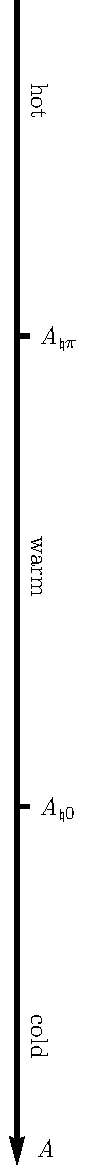
\includegraphics[height=13.6\textwidth]{bipolar-viable-arrow}
  \end{minipage}
  \begin{minipage}[b]{0.8\textwidth}
    \newcommand*{\legendtrimwidth}{0.03\textwidth}
    \newcommand*{\legendoffsetheight}{0.025\textwidth}
    
\includegraphics[
      width={\textwidth-\legendtrimwidth},
      trim={\legendtrimwidth} {-\legendoffsetheight} 0 0,
    ]{bipolar-viable-legend}
    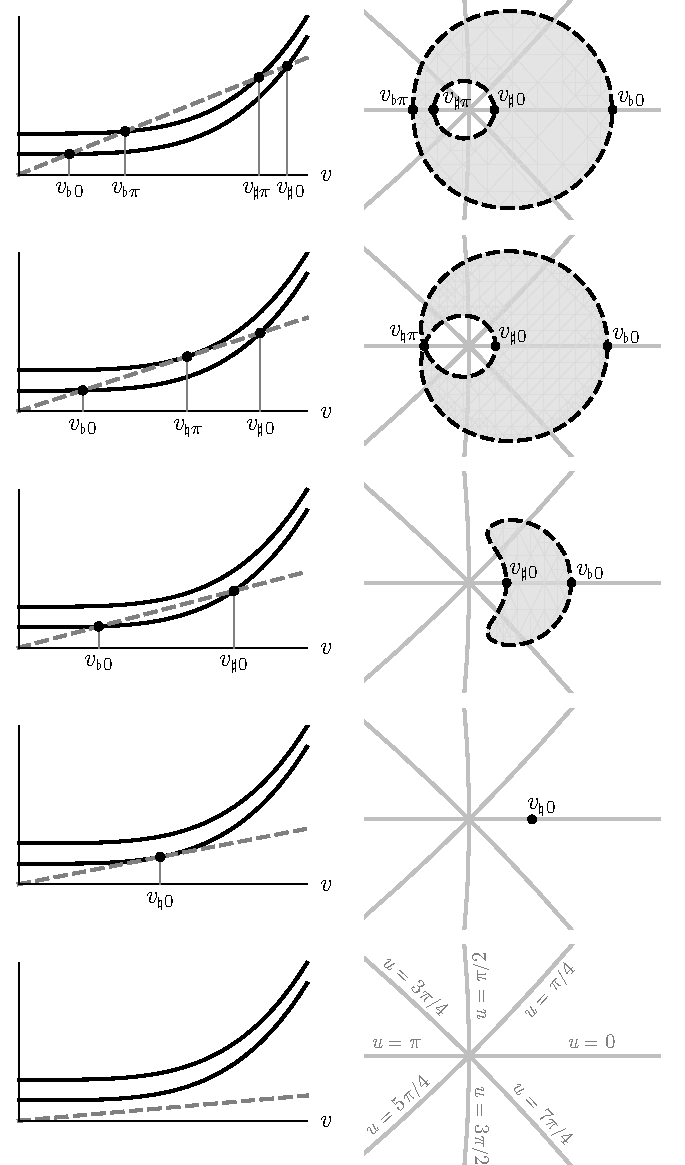
\includegraphics[width=\textwidth]{bipolar-viable}
  \end{minipage}
  \caption{
    Critical terminal points and non-viable domain~$\Phi < 0$
    for the known solution~(\ref{eq:bipolar-scaled-laplace-solution})
    and viability function~(\ref{eq:bipolar-viability-function}),
    as $A$~increases.
    In the right-hand column,
    the $u$-contours~\figurestyle{grey curves} meet
    at the positive singularity~$v = +\infty$.
  }
  \label{fig:bipolar-viable}
\end{figure}

Each of~(\ref{eq:bipolar-critical-terminal-point-pi})
and~(\ref{eq:bipolar-critical-terminal-point-0})
has zero to two roots
(ignoring~$v = 0$ for~(\ref{eq:bipolar-critical-terminal-point-0}))
depending on the size of the dimensionless group~$A$,
leading to five cases for the number of critical terminal points
and the geometry of the viable domain
(Figure~\ref{fig:bipolar-viable}):

\subsection{Five cases}
\label{sec:bipolar.viable.cases}

\begin{enumerate}
  \item
    \term{Hot regime}, $A < A_{\nat \pi}$:
    Both equations have two roots:
    $v_{\flat \pi}$ and~$v_{\sharp \pi}$
    for~(\ref{eq:bipolar-critical-terminal-point-pi})
    and
    $v_{\flat 0}$ and~$v_{\sharp 0}$
    for~(\ref{eq:bipolar-critical-terminal-point-0}),
    with~$v_{\flat 0} < v_{\flat \pi} < v_{\sharp \pi} < v_{\sharp 0}$.
    Thus there are four critical terminal points,
    having bipolar coordinates~$(0, v_{\flat 0})$, $(\pi, v_{\flat \pi})$,
    $(\pi, v_{\sharp \pi})$, and~$(0, v_{\sharp 0})$.
    The non-viable domain forms an avocado-like moat
    which surrounds an inner viable island
    (containing the singularity~$v = +\infty$)
    and is surrounded by an outer viable mainland.
  \item
    \term{Hot-to-warm transition}, $A = A_{\nat \pi}$:
    The two roots of~(\ref{eq:bipolar-critical-terminal-point-pi})
    merge together
    and the non-viable moat is pincered along~$u = \pi$,
    leaving the three critical terminal points~$(0, v_{\flat 0})$,
    $(\pi, v_{\nat \pi})$, and~$(0, v_{\sharp 0})$.
    The inner viable island and the outer viable mainland
    touch at the second of these.
  \item
    \term{Warm regime}, $A_{\nat \pi} < A < A_{\nat 0}$:
    The remaining root of~(\ref{eq:bipolar-critical-terminal-point-pi})
    disappears
    and the inner viable island is now robustly connected
    to the outer viable mainland.
    Equation~(\ref{eq:bipolar-critical-terminal-point-0}) still has two roots,
    corresponding to the two critical terminal points~%
      $(0, v_{\flat 0})$ and~$(0, v_{\sharp 0})$.
    The non-viable domain is now a crescent-shaped lake.
  \item
    \term{Warm-to-cold transition}, $A = A_{\nat 0}$:
    The two roots of~(\ref{eq:bipolar-critical-terminal-point-0})
    merge together
    and the non-viable lake dries up completely.
    The entire plane is viable,
    though a single (isolated) critical terminal point still exists
    at~$(0, v_{\nat 0})$.
  \item
    \term{Cold regime}, $A > A_{\nat 0}$:
    The remaining root of~(\ref{eq:bipolar-critical-terminal-point-0})
    disappears.
    The entire plane is viable,
    and there are no critical terminal points left.
\end{enumerate}
The two transition cases occur
when~(\ref{eq:bipolar-critical-terminal-point-pi})
and~(\ref{eq:bipolar-critical-terminal-point-0})
each have a merging of roots,
at the special values of~$A$
for which the curves~$\cosh v \pm 1$ and~$v^4 / A$
touch tangentially,
given by the extra condition
\begin{equation}
  \sinh v - \frac{4 v^3}{A} = 0.
  \label{eq:bipolar-critical-terminal-point-transition}
\end{equation}
Note how this accounts for the situation in which
the terminal curve has an indeterminate local tangent
in equation~(\ref{eq:bipolar-terminal-curve-implicit-derivative}).
By numerically solving each of~(\ref{eq:bipolar-critical-terminal-point-pi})
and~(\ref{eq:bipolar-critical-terminal-point-0})
in conjunction with the tangency condition~%
  (\ref{eq:bipolar-critical-terminal-point-transition}),
the values of~$A$ for the two transitions are determined to be
\begin{align}
  A_{\nat \pi} &= 9.06433 \eqnspace \text{hot-to-warm},
    \label{eq:bipolar-transition-a-hot-to-warm}
    \\
  A_{\nat 0} &= 9.76206 \eqnspace \text{warm-to-cold}.
    \label{eq:bipolar-transition-a-warm-to-cold}
\end{align}

\section{Boundary tracing}
\label{sec:bipolar.tracing}

In this section we write down the boundary tracing ODE
and determine the class of convex domains which can be constructed.

\subsection{Candidate boundaries}
\label{sec:bipolar.tracing.candidates}

\begin{figure}
  \newcommand*{\subfigurewidth}{0.45\textwidth}
  \newcommand*{\subfigureoffsettop}{0.08\textwidth}
  \newcommand*{\subfigureoffsetbottom}{0.04\textwidth}
  \centering
  \begin{subfigure}{\subfigurewidth}
    \centredfigurecontent[
      trim=0 {\subfigureoffsetbottom} 0 0,
    ]{bipolar-traced-boundaries-hot}{Hot regime}
  \end{subfigure}
  \hfill
  \begin{subfigure}{\subfigurewidth}
    \centredfigurecontent[
      trim=0 {\subfigureoffsetbottom} 0 0,
    ]{bipolar-traced-boundaries-warm}{Warm regime}
  \end{subfigure}
  
  \begin{subfigure}{\subfigurewidth}
    \centredfigurecontent[
      trim=0 {\subfigureoffsetbottom} 0 {-\subfigureoffsettop},
    ]{bipolar-traced-boundaries-cold}{Cold regime}
  \end{subfigure}
  \caption{
    Traced boundaries obtained by integrating~%
      (\ref{eq:bipolar-tracing-ode-coordinate-parametrisation-v}).
  }
  \label{fig:bipolar-traced-boundaries}
\end{figure}

Using~(\ref{eq:bipolar-gradient-u-component})
through~(\ref{eq:bipolar-viability-function}),
the boundary tracing ODE~(\ref{eq:tracing-ode-coordinate-parametrisation-v})
becomes
\begin{important}{equation}
  \tder{v}{u} =
    \pm
    \frac{A}{v^4}
    \sqrt{
      \roundbr[\bulkysize]{\cosh v - \cos u}^2 - \frac{v^8}{A^2}
    },
  \label{eq:bipolar-tracing-ode-coordinate-parametrisation-v}
\end{important}
which cannot be integrated analytically.
Traced boundaries determined by numerical integration
from starting points in the viable domain
are shown in Figure~\ref{fig:bipolar-traced-boundaries}.

Like the line-source case in Section~\ref{sec:polar.tracing},
the two branches of traced boundaries are segregated
by the sign of~$\td v / {\td u}$,
with the upper branch spiralling inwards
and the lower branch spiralling outwards
as one travels anticlockwise
around the singularity~$v = +\infty$.
Again, any physically sensible radiation--conduction domain
must completely surround the heat-supplying singularity without touching it,
and therefore we seek closed curves surrounding the singularity,
made from patching together the traced boundaries
given by~(\ref{eq:bipolar-tracing-ode-coordinate-parametrisation-v}).
Using similar arguments to those in Section~\ref{sec:polar.tracing},
we conclude that a necessary (but not sufficient) condition
for the convexity of the sought-after closed curve
is for it to have an upper-to-lower branch switch
at an hyperbolic critical terminal point.

\begin{figure}
  \newcommand*{\subfigurewidth}{0.35\textwidth}
  \newcommand*{\subfigureoffsetbottom}{0.08\textwidth}
  \centering
  \hspace*{\fill}
  \begin{subfigure}{\subfigurewidth}
    \centredfigurecontent[
    ]{bipolar-critical-terminal-points-hot}{Hot regime}
  \end{subfigure}
    \hfill
  \begin{subfigure}{\subfigurewidth}
    \centredfigurecontent[
    ]{bipolar-critical-terminal-points-warm_hot}{Hot-to-warm transition}
  \end{subfigure}
  \hspace*{\fill}
  
  \hspace*{\fill}
  \begin{subfigure}{\subfigurewidth}
    \centredfigurecontent[
      trim=0 {\subfigureoffsetbottom} 0 0,
    ]{bipolar-critical-terminal-points-warm}{Warm regime}
  \end{subfigure}
    \hfill
  \begin{subfigure}{\subfigurewidth}
    \centredfigurecontent[
      trim=0 {\subfigureoffsetbottom} 0 0,
    ]{bipolar-critical-terminal-points-cold_warm}{Warm-to-cold transition}
  \end{subfigure}
  \hspace*{\fill}
  
  
\includegraphics[
    width=0.85\textwidth,
    trim=0 0 0 -5,
  ]{bipolar-critical-terminal-points-legend}
  \caption{
    Local $T$-contour through each critical terminal point.
  }
  \label{fig:critical-terminal-points}
\end{figure}

The nature of the up to four critical terminal points that exist
can be determined by inspecting Figure~\ref{fig:critical-terminal-points}.
We see that those lying on the segment~$u = \pi$
(to the left of the singularity)
are of elliptic type,
as the local $T$-contour lies on the non-viable side of the terminal curve.
Only the critical terminal points lying on the segment~$u = 0$
(to the right of the singularity)
are of hyperbolic type,
and it is from these points that we might construct convex domains.
Explicitly, we have two hyperbolic critical terminal points~%
$(u, v) = (0, v_{\flat 0})$ and~$(u, v) = (0, v_{\sharp 0})$
for~$0 < A < A_{\nat 0}$ (the hot regime through to the warm regime),
which merge to become the single point~$(u, v) = (0, v_{\nat 0})$
at~$A = A_{\nat 0}$ (the warm-to-cold transition),
which then disappears for~$A > A_{\nat 0}$ (the cold regime).

\begin{figure}
  \centering
  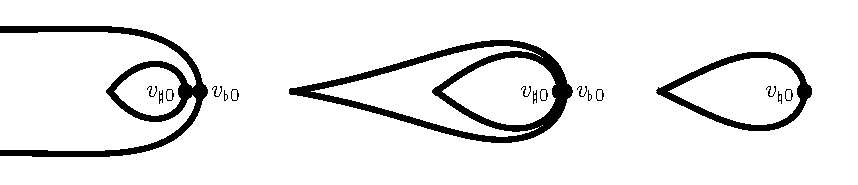
\includegraphics[width=\textwidth]{bipolar-candidates}
  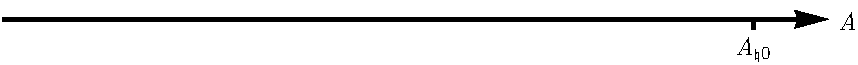
\includegraphics[width=\textwidth]{bipolar-candidates-arrow}
  \caption{
    Inner~($v_{\sharp 0}$) and outer~($v_{\flat 0}$) candidate boundaries,
    as $A$~increases.
    The two candidate boundaries become one at~$A = A_{\nat 0}$.
  }
  \label{fig:bipolar-candidates}
\end{figure}

We may therefore construct (up to) two \term{candidate boundaries}
whenever~$0 < A \le A_{\nat 0}$,
as shown in Figure~\ref{fig:bipolar-candidates}.
An \term{outer candidate boundary} is constructed
by performing an upper-to-lower branch switch at~$(0, v_{\flat 0})$,
i.e.~by taking the upper branch for~$-\pi < u \le 0$
and joining it to the lower branch for~$0 \le u < \pi$.
An \term{inner candidate boundary} is produced likewise
from the point~$(0, v_{\sharp 0})$.
The two boundaries merge together
when $v_{\flat 0}$ and~$v_{\sharp 0}$ merge
at the warm-to-cold transition~$A = A_{\nat 0}$.

The inner candidate boundary forms a closed loop
and appears to be convex over the entire interval~$0 < A \le A_{\nat 0}$.
The outer candidate boundary only forms a closed loop
if $A$~is sufficiently large,
but in the next section we show that this is irrelevant
because the outer candidate boundary is always non-convex.

\subsection{Convexity of the candidate boundaries}
\label{sec:bipolar.tracing.convex}

We first consider the inner candidate boundary,
which always forms a closed loop
by way of its two branches meeting in a corner
at~$(u, v) = (\mp\pi, v_\End)$ on the left
(Figure~\ref{fig:bipolar-inner-candidate}).
While this boundary appears to be convex for all~$A \le A_{\nat 0}$,
we cannot be certain until a global curvature analysis is performed
like that of Section~\ref{sec:polar.convex.beyond}.

\begin{figure}
  \centredfigurecontent[width=0.45\textwidth]{%
    bipolar-inner-candidate%
  }{
    Bipolar coordinates of the left-hand and right-hand extremities
    of an inner candidate boundary.
  }
\end{figure}

From the coordinate transformations
we obtain the orthonormal basis vectors
\begin{align}
  \basisvec{u} &= -\scalefac S \basisvec{x} + \scalefac C \basisvec{y},
    \label{eq:u-basis-vector-bipolar} \\
  \basisvec{v} &= -\scalefac C \basisvec{x} - \scalefac S \basisvec{y},
    \label{eq:v-basis-vector-bipolar}
\end{align}
where
\begin{align}
  S &= \sin u \sinh v,
    \label{eq:bipolar-abbreviation-s} \\
  C &= \cos u \cosh v - 1,
    \label{eq:bipolar-abbreviation-c}
\end{align}
and $\scalefac$~is the dimensionless scale factor~%
  (\ref{eq:dimensionless-scale-factor-bipolar}).
We consider a curve parametrised in the form~$v = v (u)$,
and let primes denote $u$-differentiation.
After some algebra, we find that
the basis vectors~(\ref{eq:u-basis-vector-bipolar})
and~(\ref{eq:v-basis-vector-bipolar})
change according to
\begin{align}
  (\basisvec{u})'
  &= -\scalefac^2 C D \basisvec{x} - \scalefac^2 S D \basisvec{y}
  = +\scalefac D \basisvec{v},
    \label{eq:u-basis-vector-u-derivative-bipolar} \\
  (\basisvec{v})'
  &= +\scalefac^2 S D \basisvec{x} - \scalefac^2 C D \basisvec{y}
  = -\scalefac D \basisvec{u},
    \label{eq:v-basis-vector-u-derivative-bipolar}
\end{align}
where
\begin{equation}
  D = \sinh v - v' \sin u.
  \label{eq:bipolar-abbreviation-d}
\end{equation}
Now, from the differential displacement
\begin{equation}
  \td\positionvec =
    \scalefac \td u \basisvec{u} + \scalefac \td v \basisvec{v},
  \label{eq:differential-displacement-bipolar}
\end{equation}
we have the velocity
\begin{equation}
  \positionvec' = \tder{\positionvec}{u} =
    \scalefac \basisvec{u} + \scalefac v' \basisvec{v}.
  \label{eq:velocity-vector-bipolar-by-u}
\end{equation}
Taking another $u$-derivative,
and using~(\ref{eq:u-basis-vector-u-derivative-bipolar})
and~(\ref{eq:v-basis-vector-u-derivative-bipolar})
to simplify,
we obtain the acceleration
\begin{equation}
  \positionvec'' = \tder[2]{\positionvec}{u} =
    - \scalefac^2 (D v' + E) \basisvec{u}
    + \scalefac (v'' - \scalefac E v' + \scalefac D) \basisvec{v},
  \label{eq:acceleration-vector-bipolar-by-u}
\end{equation}
where
\begin{equation}
  E = v' \sinh v + \sin u.
  \label{eq:bipolar-abbreviation-e}
\end{equation}
A quantity having the same sign changes as curvature is therefore
\begin{equation}
  \kappa = \basisvec{z} \dotp (\positionvec' \crossp \positionvec'') =
    \scalefac^3
    \squarebr*{D \roundbr*{1 + {v'}^2} + \frac{v''}{\scalefac}}.
  \label{eq:kappa-bipolar-by-u}
\end{equation}
Inspecting
Figures~\ref{fig:bipolar-candidates} and~\ref{fig:bipolar-inner-candidate}
once more,
we note again that
the inner candidate boundary appears to be always convex.
Certainly the rotund right-hand end is convex.
However, while the tip at the left-hand end looks to be a convex corner,
there remains the possibility
that it could actually be a non-convex spike,
similar to Figure~\hyperref[fig:plane-domains]{\ref*{fig:plane-domains}c}
(although much more subtle).
To test this,
we evaluate~(\ref{eq:kappa-bipolar-by-u}),
first using the traced boundary derivative~%
  (\ref{eq:bipolar-tracing-ode-coordinate-parametrisation-v})
for~$v'$,
and then substituting~$u = \mp\pi$
(which is the location of the tip for each branch).
We obtain
\begin{equation}
  \eval*{\kappa}_{u = \mp\pi} =
    \frac{2 A^2}{v^9}
    \roundbr*{-2 + v \tanh\frac{v}{2}},
    \label{eq:bipolar-traced-boundary-kappa-bipolar-by-u-tip}
\end{equation}
which changes sign at the positive solution to the transcendental equation
\begin{equation}
  \frac{v}{2} \tanh\frac{v}{2} = 1,
\end{equation}
numerically
\begin{equation}
  v = v_\infl = 2.39936.
  \label{eq:bipolar-v-inflection-tip}
\end{equation}
The inner candidate boundary will therefore be convex
if and only if its tip at the left-hand end~$(u, v) = (\mp\pi, v_\End)$
either coincides with or lies to the right of~$(u, v) = (\mp\pi, v_\infl)$.
Algebraically, we will have convexity if and only if~$v_\End \ge v_\infl$.
We see from Figure~\ref{fig:bipolar-candidates}
that the tip is furthest to the left when~$A = A_{\nat 0}$
(when the inner and outer candidates merge),
and in this worst-case scenario
the tip coordinate computes to~$v_\End = 2.20618$,
which is \emph{less than}
the critical value~(\ref{eq:bipolar-v-inflection-tip}).
It follows that the inner candidate boundary is in fact non-convex for
\begin{equation}
  A_\infl < A \le A_{\nat 0},
  \label{eq:bipolar-inner-candidate-non-convex-a-interval}
\end{equation}
where the lower bound~$A_\infl$ is the value of~$A$ at which
\begin{equation}
  v_\End = v_\infl,
  \label{eq:bipolar-inner-candidate-a-inflection-equation}
\end{equation}
corresponding to inflection occurring exactly at the tip.
Using the bisection algorithm we obtain
\begin{equation}
  A_\infl = 9.76036,
  \label{eq:bipolar-inner-candidate-a-inflection}
\end{equation}
which is extremely close to the upper value~$A_{\nat 0} = 9.76206$:
indeed the width of the interval~%
  (\ref{eq:bipolar-inner-candidate-non-convex-a-interval})
is an exceedingly minuscule~$1.7 \times 10^{-3}$.
It is pure coincidence that
among the entire interval~$0 < A \le A_{\nat 0}$
of inner candidate boundaries,
such a tiny fraction of them should be non-convex.
While this is most remarkable from a theoretical perspective,
we note that there is little significance in practice,
as the amount of self-viewing radiation is exceptionally tiny.

For the outer candidate boundary,
we return again to Figure~\ref{fig:bipolar-candidates}.
First we rule out the candidates with $A$~too small,
as these do not form a closed loop.
Of the remaining outer candidate boundaries
(which do form a closed loop),
we observe that the left-hand tip at best
coincides with the tip of the $A = A_{\nat 0}$~boundary
(when the inner and outer candidates merge).
As we have just seen from the analysis of the inner candidate,
this $A = A_{\nat 0}$~boundary is non-convex.
Hence, the outer candidate boundary
never forms a convex closed loop.

While it is possible to quantify the amount of self-viewing radiation
to determine non-convex yet practical domains
(both for the minuscule continuum~%
  (\ref{eq:bipolar-inner-candidate-non-convex-a-interval})
of inner candidate boundaries
and for the outer candidate boundaries that form a closed loop),
we omit such an analysis here
for the same reasons as given in Section~\ref{sec:polar.convex.self-viewing}.

\subsection{Numerical verification}
\label{sec:bipolar.tracing.verification}

\begin{figure}
  \centering
  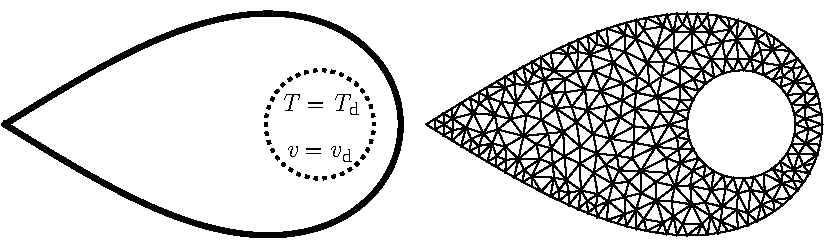
\includegraphics[width=0.968\textwidth]{bipolar-verification-domain-mesh}
  
\includegraphics[width=\textwidth]{line-verification-domain-mesh-legend}
  \caption{
    Selected domain and finite element mesh for numerical verification.
  }
  \label{fig:bipolar-verification-domain-mesh}
\end{figure}

\begin{figure}
  \centredfigurecontent[width=0.56\textwidth]{%
    bipolar-inner-candidate-with-circle%
  }{
    Circle~$v = v_{\sharp 0}$~\figurestyle{grey},
    which touches the inner candidate boundary~\figurestyle{black}
    at the critical terminal point~$(u, v) = (0, v_{\sharp 0})$.
  }
\end{figure}

For numerical verification using finite elements,
we consider the conduction--radiation domain shown
in Figure~\ref{fig:bipolar-verification-domain-mesh}.
The radiation boundary is the inner candidate boundary for~$A = 9.76$.
The heat-supplying singularity~$v = +\infty$
we have replaced with an equivalent Dirichlet condition~$T = T_\dir$
along a circle~$v = v_\dir$,
where~$T_\dir = v_\dir$
per the known solution~(\ref{eq:bipolar-scaled-laplace-solution}).
It is necessary to choose~$v_\dir > v_{\sharp 0}$
so that the Dirichlet boundary is a strictly interior one,
since the circle~$v = v_{\sharp 0}$ touches
the right-hand end of the radiation boundary
at the critical terminal point~$(0, v_{\sharp 0})$
(Figure~\ref{fig:bipolar-inner-candidate-with-circle}).
Here we have selected~$v_\dir = 1.1 v_{\sharp 0} = 4.26$,
so that the constant-temperature boundary
of Figure~\ref{fig:bipolar-verification-domain-mesh}
is a circle of radius~$0.028$.

We again use \software{Mathematica}'s \code{NDSolve\`{}FEM\`{}},
generating a mesh with approximately 500~triangular elements.
The relevant conduction--radiation BVP is solved numerically,
consisting of Laplace's equation in the interior,
the radiation condition~(\ref{eq:bipolar-scaled-radiation-boundary-condition})
on the external boundary,
and the aforesaid Dirichlet condition on the interior boundary.
Comparing the resulting numerical solution
to the known exact solution~(\ref{eq:bipolar-scaled-laplace-solution}),
we find that the maximum relative error throughout the mesh
is of the order~$10^{-3}$
(Figure~\ref{fig:bipolar-verification}).

\begin{figure}
  \newcommand*{\subfigurewidth}{0.42\textwidth}
  \centering
  \hspace*{\fill}
  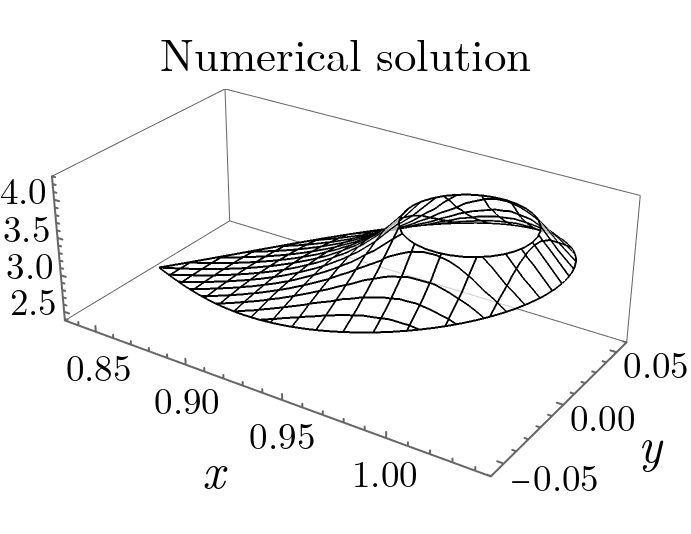
\includegraphics[width=\subfigurewidth]{bipolar-verification-solution}
    \hfill
  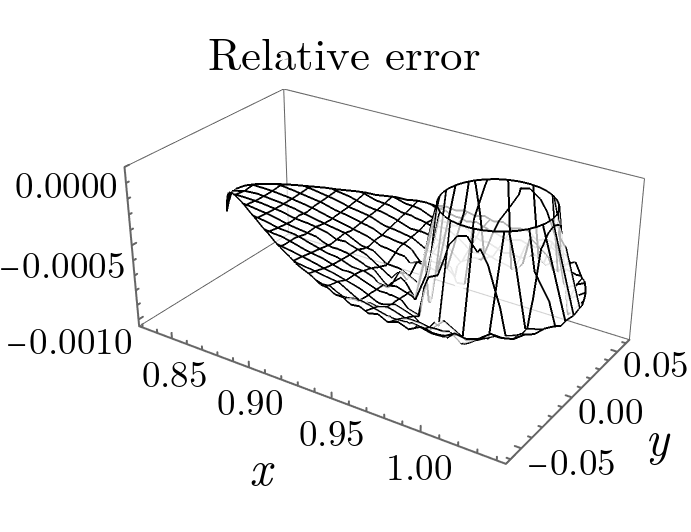
\includegraphics[width=\subfigurewidth]{bipolar-verification-relative-error}
  \hspace*{\fill}
  \caption{
    Numerical verification.
  }
  \label{fig:bipolar-verification}
\end{figure}

\section{Physical range}
\label{sec:bipolar.physical}

In this section, we determine for various quantities
the physical range that can be achieved over the continuum
\begin{equation}
  0 < A \le A_{\nat 0}
  \label{eq:bipolar-inner-candidate-existence-interval}
\end{equation}
of inner candidate boundaries.
For the purposes of this analysis,
we shall ignore the issue of non-convexity
in the minute subinterval~%
  (\ref{eq:bipolar-inner-candidate-non-convex-a-interval}),
with the special value~$A_{\nat 0}$
serving as an algebraically convenient approximation
for the upper limit~$A_\infl$ of convexity.
We return here to unscaled variables,
restoring the \scalingmarks{} which were dropped
from (\ref{eq:bipolar-scaled-radiation-boundary-condition})~onwards.

\subsection{Asymmetry}
\label{sec:bipolar.physical.asymmetry}

Inspecting the inner candidate boundaries
of Figure~\ref{fig:bipolar-candidates},
we see that an increase in the dimensionless group~$A$
results in an elongation of the characteristic teardrop shape.
This makes sense physically.
The bipolar solution~(\ref{eq:bipolar-laplace-solution})
to Laplace's equation
arises from the superposition of equal and opposite line sources
at~$(x, y) = (\pm a, 0)$,
so we may think of it as a perturbation of
the radial line-source solution~(\ref{eq:line-laplace-solution})
caused by the introduction of an opposite line source at distance~$2 a$.
Since the dimensionless group~$A$
is inversely proportional to the length scale~$a$
(see~(\ref{eq:bipolar-dimensionless-group})),
an increase in~$A$ brings the second line source (which is cold)
closer to the first line source (which is hot),
thus increasing the amount of asymmetry.

It is no coincidence that we have a non-viable moat
separating an inner viable island from an outer viable mainland,
both for the line-source solution of Chapter~\ref{ch:polar}
and for the present bipolar solution, when $A$ is sufficiently small.
The limiting case of~$A = 0$
corresponds to the second line source being infinitely far removed,
i.e.~a reduction to the purely radial case.

The inner candidate boundary for the bipolar solution
is in fact a deformed version
of the trivial circular traced boundary~($r = r_\flat$)
that exists on the inner viable island,
in the hot regime of the line-source solution
(Section~\ref{sec:polar.tracing.hot}).
In the limiting $A = 0$~case,
the inner candidate boundary would be a circle
centred on the singularity~$v = +\infty$,
but for~$A > 0$,
the presence of the negative singularity
causes the inner candidate boundary to deviate
from perfectly circularity.
The amount of asymmetry may be quantified
through the ratio of distances from
the ideal centre~$(x, y) = (+a, 0)$
(which is the singularity~$v = +\infty$)
to each of the left-hand and right-hand extremities
(which have bipolar coordinates $(\mp\pi, v_\End)$ and~$(0, v_{\sharp 0})$
respectively; see Figure~\ref{fig:bipolar-inner-candidate}).
Thus
\begin{align*}
  \textq{Asymmetry}
  &=
    \frac{a - x_\End}{x_{\sharp 0} - a}
      \\[\tallspace]
  &=
    \frac{
      1 - \sinh v_\End / (\cosh v_\End - \cos(\mp\pi))
    }{
      \sinh v_{\sharp 0} / (\cosh v_{\sharp 0} - \cos 0) - 1
    }
      \\[\tallspace]
  &=
    \frac{\exp v_{\sharp 0} - 1}{\exp v_\End + 1}.
    \yesnumber
    \label{eq:bipolar-inner-candidate-asymmetry}
\end{align*}
The asymmetry will only become significant
if the negative line source has been brought
sufficiently close to the positive one.
From Figure~\ref{fig:bipolar-inner-candidate-asymmetry}
we see that this only occurs towards the colder end of the warm regime.

\begin{figure}
  \centredfigurecontent[width=0.6\textwidth]{%
    bipolar-inner-candidate-asymmetry%
  }{
    Asymmetry~(\ref{eq:bipolar-inner-candidate-asymmetry})
    of the inner candidate boundary,
    as $A$~increases.
    No inner candidate boundary exists
    in the cold regime~($A > A_{\nat 0}$).
  }
\end{figure}

\subsection{Temperature}
\label{sec:bipolar.physical.temperature}

Here we perform a similar analysis
to Section~\ref{sec:polar.physical.temperature},
to determine the physical temperatures that can be realised
by inner candidate boundaries of a prescribed size.
For simplicity,
we take the radius of the circle~$v = v_{\sharp 0}$
(Figure~\ref{fig:bipolar-inner-candidate-with-circle})
as our fixed reference length.
From~(\ref{eq:bipolar-circle-v})
we see that this radius is given by
\begin{equation}
  r_{\sharp 0} = a \csch v_{\sharp 0},
  \label{eq:bipolar-r-sharp-0}
\end{equation}
so that the length scale (intrinsic to the bipolar coordinate system) is
\begin{equation}
  a = r_{\sharp 0} \sinh v_{\sharp 0}.
  \label{eq:bipolar-length-scale-in-terms-of-r-sharp-0}
\end{equation}
By construction, the bipolar coordinate~$v_{\sharp 0}$
is a root of the equation~(\ref{eq:bipolar-critical-terminal-point-0})
for critical terminal points along~$u = 0$;
therefore we have
\begin{equation}
  A = \frac{{v_{\sharp 0}}^4}{\cosh v_{\sharp 0} - 1}.
  \label{eq:bipolar-dimensionless-group-in-terms-of-r-sharp-0}
\end{equation}
After rearranging~(\ref{eq:bipolar-dimensionless-group}) for~$T_0$,
we may use~(\ref{eq:bipolar-length-scale-in-terms-of-r-sharp-0})
and~(\ref{eq:bipolar-dimensionless-group-in-terms-of-r-sharp-0})
to obtain
\begin{equation}
  T_0 =
    \roundbr*{
      \frac{
        \cosh v_{\sharp 0} - 1
      }{
        c r_{\sharp 0} {v_{\sharp 0}}^4 \sinh v_{\sharp 0}
      }
    }^{1/3}
  \label{eq:bipolar-temperature-scale-in-terms-of-r-sharp-0}
\end{equation}
for the temperature scale
of the known solution~(\ref{eq:bipolar-laplace-solution}).
It follows that the physical temperature
along the reference circle~$v = v_{\sharp 0}$
is
\begin{align*}
  T_{\sharp 0}
  &= T_0 \cdot v_{\sharp 0} \\
  &=
    \roundbr*{
      \frac{
        \cosh v_{\sharp 0} - 1
      }{
        c r_{\sharp 0} v_{\sharp 0} \sinh v_{\sharp 0}
      }
    }^{1/3}
    \\
  &=
    \roundbr*{
      \frac{\omega (v_{\sharp 0})}{c r_{\sharp 0}}
    }^{1/3},
    \yesnumber
    \label{eq:bipolar-t-sharp-0-in-terms-of-r-sharp-0}
\end{align*}
where $\omega$~is the dimensionless auxiliary function
\begin{equation}
  \omega (v) = \frac{\cosh v - 1}{v \sinh v}
  \label{eq:bipolar-auxiliary-function}
\end{equation}
shown in Figure~\ref{fig:bipolar-auxiliary-function}.

\begin{figure}
  \centredfigurecontent[width=0.55\textwidth]{%
    bipolar-auxiliary-function%
  }{
    Auxiliary function~(\ref{eq:bipolar-auxiliary-function}).
  }
\end{figure}

Now, as the dimensionless group~$A$
runs through the interval~%
  (\ref{eq:bipolar-inner-candidate-existence-interval})
of all inner candidate boundaries,
i.e.~from the limiting extreme~$A = 0$ of the hot regime
up to the warm-to-cold transition~$A = A_{\nat 0} = 9.76206$,
the quantity~$v_{\sharp 0}$ decreases from infinity
down to the transition value~$v_{\nat 0} = 3.83002$;
this can be seen from the left-hand column
of Figure~\ref{fig:bipolar-viable}.
It can be shown that $\omega$~is a decreasing function,
whence we have
\begin{equation}
  \omega (\infty) < \omega (v_{\sharp 0}) \le \omega (v_{\nat 0}).
  \label{eq:bipolar-inner-candidate-omega-interval}
\end{equation}
The upper bound may in fact be simplified to~$1/4$,%
\footnote{
  This would not have happened
  had we chosen $A_\infl$ instead of the special value~$A_{\nat 0}$
  for the upper bound of the interval~%
  (\ref{eq:bipolar-inner-candidate-existence-interval}).
}
so we have
\begin{equation}
  0 < \omega (v_{\sharp 0}) \le 1/4.
  \label{eq:bipolar-inner-candidate-omega-interval-evaluated}
\end{equation}
Therefore,
the unscaled temperature~(\ref{eq:bipolar-t-sharp-0-in-terms-of-r-sharp-0})
spans the interval
\[
  0
    <
  T_{\sharp 0}
    \le
  \roundbr*{\frac{1}{4 c r_{\sharp 0}}}^{1/3},
\]
or
\begin{equation}
  0
    <
  T_{\sharp 0}
    \le
  \frac{1}{2^{2/3}}
  \roundbr*{\frac{\conduc}{\emiss \stefan r_{\sharp 0}}}^{1/3}.
  \label{eq:bipolar-inner-candidate-t-sharp-0-interval}
\end{equation}
It is interesting to note that this interval
perfectly complements the analogous line-source result~%
  (\ref{eq:line-traced-boundary-hot-convex-t-sharp-interval}),
whose lower bound is precisely the upper bound here
(with $r_\sharp$ in place of~$r_{\sharp 0}$).
For the PVC parameter values
of Section~\ref{sec:polar.physical.temperature},
the interval~(\ref{eq:bipolar-inner-candidate-t-sharp-0-interval})
evaluates to $\SI{0}{\kelvin} < T_{\sharp 0} \le \SI{277}{\kelvin}$.

At first glance one is tempted to conclude that physically,
the introduction of a negative image source
has the effect of extending the interval of possible temperatures
down to absolute zero.
However, upon closer inspection we see that
the exact agreement between the bounds is in fact fortuitous,
as it is the \emph{lower} bound
of~(\ref{eq:bipolar-inner-candidate-t-sharp-0-interval})
which is realised
when the bipolar solution reduces to the line-source solution
at~$A = 0$.
The upper bound is instead realised at
the warm-to-cold transition~$A = A_{\nat 0}$.

While the perfect agreement between the temperature bounds is a coincidence,
there is still reason for them to be of similar magnitude.
The physical ranges of Section~\ref{sec:polar.physical}
(for the line-source solution)
were derived for convex domains
constructed on the outer viable mainland of the hot regime.
These convex domains were constructed
in Section~\ref{sec:polar.convex.construction}
by making protrusions from the outer terminal curve~$r = r_\sharp$.
The bipolar inner candidate boundaries here are an analogue
\emph{not} of those protrusions on the outer viable mainland,
but of the circular traced boundary~$r = r_\flat$,
which was the sole convex boundary of the inner viable island.
That boundary was not analysed further due to its trivial shape,
but one may show that its corresponding temperature interval
is precisely~(\ref{eq:bipolar-inner-candidate-t-sharp-0-interval})
with $r_\flat$ in place of~$r_{\sharp 0}$.
Thus, the true reason for the agreement between the temperature bounds
is the similarity
between the bipolar inner candidate
and the line-source inner circle~$r = r_\flat$.

\subsection{Power per unit length}
\label{sec:bipolar.physical.power}

Returning now to the bipolar inner candidate,
the rate at which heat is generated internally
(and thus expelled via radiation from the boundary)
is fixed by the strength of the singularity~$v = +\infty$,
corresponding to the positive term
of~(\ref{eq:bipolar-laplace-solution-terms}).
Physically this is identical
to the fundamental line-source~(\ref{eq:line-laplace-solution}),
so we again have~(\ref{eq:line-power-per-length-fundamental}), i.e.
\begin{equation}
  p = 2 \pi \conduc T_0,
  \label{eq:line-power-per-length-fundamental-repeat}
\end{equation}
for the power dissipated per unit length.
Using~(\ref{eq:bipolar-temperature-scale-in-terms-of-r-sharp-0}),
this becomes
\begin{align*}
  p
  &=
    2 \pi \conduc
    \roundbr*{
      \frac{
        \cosh v_{\sharp 0} - 1
      }{
        c r_{\sharp 0} {v_{\sharp 0}}^4 \sinh v_{\sharp 0}
      }
    }^{1/3}
      \\[\tallspace]
  &=
    \frac{2 \pi \conduc}{(c r_{\sharp 0})^{1/3}}
    \roundbr*{
      \frac{
        \omega (v_{\sharp 0})
      }{
        {v_{\sharp 0}}^3
      }
    }^{1/3}.
      \yesnumber
      \label{eq:bipolar-power-per-length}
\end{align*}
As before, $\omega (v_{\sharp 0})$~runs through the interval~%
  (\ref{eq:bipolar-inner-candidate-omega-interval-evaluated})
as $v_{\sharp 0}$~decreases from infinity down to~$v_{\nat 0} = 3.83002$.
Therefore we have the interval
\[
  0 < p \le
    \frac{2 \pi \conduc}{(c r_{\sharp 0})^{1/3}}
    \roundbr*{
      \frac{
        1/4
      }{
        {v_{\nat 0}}^3
      }
    }^{1/3}
\]
in power per unit length, or
\begin{equation}
  0 < p \le
    \frac{2^{1/3}}{v_{\nat 0}}
    \frac{\pi \conduc^{4/3}}{(\emiss \stefan r_{\sharp 0})^{1/3}},
\end{equation}
evaluating to $0 < p \le \SI{82}{\watt \per\metre}$
for the parameters from the PVC example
of Section~\ref{sec:polar.physical.temperature}.

Unlike the temperature interval~%
  (\ref{eq:bipolar-inner-candidate-t-sharp-0-interval}),
the upper bound here does not coincide exactly
with the lower bound of~%
  (\ref{eq:line-traced-boundary-hot-convex-power-per-length-interval})
for the line-source solution.
As noted in Section~\ref{sec:bipolar.physical.temperature},
perfect agreement would be coincidental,
but we should nevertheless expect a similar order of magnitude.
A quick calculation shows that the prefactor here is
\[
  \frac{2^{1/3}}{v_{\nat 0}} = 0.32896,
\]
a mere $\SI{4}{\percent}$~more than the prefactor
\[
  \frac{1}{2^{5/3}} = 0.31498
\]
for the lower bound of~%
  (\ref{eq:line-traced-boundary-hot-convex-power-per-length-interval}).

\section{Summary}
\label{sec:bipolar.summary}

In this chapter, we have used boundary tracing
to analyse the conduction--radiation problem
for the bipolar solution~(\ref{eq:bipolar-laplace-solution}).
After developing the bipolar coordinate system
from first principles
in order to better understand the physics,
we have determined how the critical terminal points merge and disappear
as the sole dimensionless group~(\ref{eq:bipolar-dimensionless-group})
increases.
Accordingly, we have identified five cases
for the topology of the viable domain,
being three regimes separated by two transitions.

A continuum of so-called inner candidate boundaries can be constructed,
which have the potential to represent convex conduction--radiation domains.
Through further analysis we have shown that
while the majority of these candidates are indeed convex,
a tiny fraction of them are actually self-viewing
(but to a degree that is likely negligible in practice).
The validity of the produced domains has been confirmed
by comparing finite element solutions for the conduction--radiation BVP
against the exact solution~(\ref{eq:bipolar-laplace-solution}).

Finally we have determined the physical ranges
for asymmetry, temperature, and power per unit length
that can be achieved
among candidate boundaries of a prescribed size;
moreover, we have reconciled these results
with those in Section~\ref{sec:polar.physical}
for the purely radial line-source solution,
which is a limiting case of the bipolar solution
when the negative image source is infinitely far removed.


\part{Capillarity}
\label{pt:capillarity}

\backmatter
\bookmarksetup{startatroot}

\bibliographystyle{conway}
\bibliography{bibliography}

\end{document}
